\RequirePackage{rotating}
\documentclass[format=acmsmall, natbib=false, review=false, authordraft=false, anonymous=false, screen=true]{acmart}
\settopmatter{printccs=false,printacmref=false}

% using biblatex
\let\citename\relax
\RequirePackage[abbreviate=true,
 dateabbrev=true,
 natbib=true,
 isbn=false,
 doi=false,
 eprint=false,
 urldate=comp,
 url=false,
 maxbibnames=9,
 maxcitenames=2,
 backref=false,
 backend=biber,
 style=ACM-Reference-Format,
language=american]{biblatex}

\addbibresource{cscw-comic.bib}
\addbibresource{hari-cscw-comic.bib}
\renewcommand{\bibfont}{\Small}


\newcommand{\hs}[1]{\textcolor{red}{#1}}
\usepackage{enumitem}

\usepackage{url}
\urlstyle{tt}
\usepackage{wasysym}
\usepackage{numprint} %in preamble % nice numbers in tables 

\usepackage{wrapfig}
\usepackage{booktabs} % For formal tables
\usepackage{cleveref} % for better references
\usepackage{graphicx,subfig,caption}
\usepackage[ruled]{algorithm2e} % For algorithms
\renewcommand{\algorithmcfname}{ALGORITHM}
\SetAlFnt{\small}
\SetAlCapFnt{\small}
\SetAlCapNameFnt{\small}
\SetAlCapHSkip{0pt}
\IncMargin{-\parindent}

\usepackage{subfig} % subcaptions
\usepackage{wasysym} % smiley faces
\usepackage{xfrac}

% Metadata Information
% \acmJournal{TWEB}
% \acmVolume{9}
% \acmNumber{4}
% \acmArticle{39}
% \acmYear{2010}
% \acmMonth{3}
% \copyrightyear{2009}
%\acmArticleSeq{9}

% Copyright
\setcopyright{acmcopyright}
% \setcopyright{acmlicensed}
%\setcopyright{rightsretained}
%\setcopyright{usgov}
%\setcopyright{usgovmixed}
%\setcopyright{cagov}
%\setcopyright{cagovmixed}
%\setcopyright{none}

% DOI
% \acmDOI{0000001.0000001}
\acmDOI{}

% % Paper history
\acmConference[]{Submitted to CSCW}{2019}{Austin, TX.}
% \received{February 2007}
% \received[revised]{March 2009}
% \received[accepted]{June 2009}


% Document starts
\begin{document}
% Title portion. Note the short title for running heads
\title[The Abstract Comic Form for Persuasion]{Should We Use an Abstract Comic Form to Persuade? Experiments with Online Charitable Donation}


\author{Ziang Xiao}
\email{zxiao5@illinois.edu}
\affiliation{%
 \institution{University of Illinois at Urbana-Champaign}
 \department{Computer Science}
 \city{Urbana}
 \state{IL}
 \postcode{61801}
 \country{USA}}
\author{Po-Shiun Ho}
\email{pho11@illinois.edu}
\affiliation{%
 \institution{University of Illinois at Urbana-Champaign}
 \department{Computer Science}
 \city{Urbana}
 \state{IL}
 \postcode{61801}
 \country{USA}}
\author{Xinran Wang}
\email{xinranw5@illinois.edu}
\affiliation{%
 \institution{University of Illinois at Urbana-Champaign}
 \department{Computer Science}
 \city{Urbana}
 \state{IL}
 \postcode{61801}
 \country{USA}}
\author{Karrie Karahalios}
\email{kkarahal@illinois.edu}
\affiliation{%
 \institution{University of Illinois at Urbana-Champaign}
 \department{Computer Science}
 \city{Urbana}
 \state{IL}
 \postcode{61801}
 \country{USA}}
\author{Hari Sundaram}
\email{hs1@illinois.edu}
\affiliation{%
 \institution{University of Illinois at Urbana-Champaign}
 \department{Computer Science}
 \city{Urbana}
 \state{IL}
 \postcode{61801}
 \country{USA}}


%!TEX root = cscw2019-comic.tex
\begin{abstract}
This paper examines the use of the abstract comic form for persuading online charitable donations. Persuading individuals to contribute to charitable causes online is hard and responses to the appeals are typically low; charitable donations share the structure of public goods dilemmas where the rewards are distant and non-exclusive. In this paper, we examine if comics in abstract form are more persuasive than in the plain text form. Drawing on a rich literature on comics, we synthesized a three-panel abstract comic to create our appeal. We conducted a between-subject study with 307 participants from Amazon Mechanical Turk on the use of abstract comic form to appeal for charitable donations. As part of our experimental procedure, we sought to persuade individuals to contribute to a real charity focused on Autism research with monetary costs. We compared the average amount of donation to the charity under three conditions: the plain text message, an abstract comic that includes the plain text, and an abstract comic that additionally includes the social proof. We use Bayesian modeling to analyze the results, motivated by model transparency and its use in small-sized studies. Our experiments reveal that the message in abstract comic form elicited significantly more donations than text form (medium to large effect size=0.59). Incorporating social proof in the abstract comic message did not show a significant effect. Our studies have design implications: non-profits and governmental agencies interested in alleviating public goods dilemmas that share a similar structure to our experiment (single-shot task, distant, non-exclusive reward) ought to consider including messages in the abstract comic form as part of their online fund-raising campaign.
\end{abstract}


%
% The code below should be generated by the tool at
% http://dl.acm.org/ccs.cfm
% Please copy and paste the code instead of the example below.
%
% \begin{CCSXML}
% <ccs2012>
%  <concept>
%   <concept_id>10010520.10010553.10010562</concept_id>
%   <concept_desc>Computer systems organization~Embedded systems</concept_desc>
%   <concept_significance>500</concept_significance>
%  </concept>
%  <concept>
%   <concept_id>10010520.10010575.10010755</concept_id>
%   <concept_desc>Computer systems organization~Redundancy</concept_desc>
%   <concept_significance>300</concept_significance>
%  </concept>
%  <concept>
%   <concept_id>10010520.10010553.10010554</concept_id>
%   <concept_desc>Computer systems organization~Robotics</concept_desc>
%   <concept_significance>100</concept_significance>
%  </concept>
%  <concept>
%   <concept_id>10003033.10003083.10003095</concept_id>
%   <concept_desc>Networks~Network reliability</concept_desc>
%   <concept_significance>100</concept_significance>
%  </concept>
% </ccs2012>
% \end{CCSXML}
%
% \ccsdesc[500]{Computer systems organization~Embedded systems}
% \ccsdesc[300]{Computer systems organization~Redundancy}
% \ccsdesc{Computer systems organization~Robotics}
% \ccsdesc[100]{Networks~Network reliability}

%
% End generated code
%


\keywords{abstract comics, persuasion, information framing, social proof, hierarchical bayesian models}




\maketitle

% The default list of authors is too long for headers.
\section{introduction}
\label{sec:introduction}
Are persuasive text messages more effective when expressed in comic form? Text messages abound, asking us to act, either towards personal wellness goals (e.g. in an exercise app:``you need 2,000 more steps to reach 10,000 steps for the day''), reminders (e.g. push notifications from a task tracking app: ``pick up prescription from the pharmacy at 6PM''), or appeals from charities online (e.g. from a Wikipedia campaign on the Wikipedia homepage: ``If everyone reading this donated \$5 our fundraiser would end today. Please donate to keep Wikipedia free.''). Making these short text messages more effective has important implications in stimulating behavior, especially for non-profits and governmental agencies interested in alleviating public goods dilemmas.

There is a rich history of prior work in psychology that has examined how variations in the construction of the text message alter decisions. In a seminal paper,~\textcite{tversky1981framing} examined information framing: can we elicit different decisions, by describing the outcome either as a loss or a gain, even though the two messages are indistinguishable in terms of expected utility? They found that individuals are risk-seeking when confronted with certain loss and risk-averse in the presence of gains. Cialdini examined the introduction of social proofs in two different contexts: towel re-use in hotels~\parencite{goldstein2008room}, reduction of power consumption~\parencite{schultz2007constructive}. In the former study, replacing the standard text message in hotels asking the customer to re-use towels with the social proof (e.g. ``75\% of the people in this hotel have re-used their towels'') increased towel re-use. The latter study had an intriguing result---while introducing the social proof in the message \textit{did not} reduce overall energy consumption, adding emoticons to the message with the social proof made a difference. Specifically, they added a smiley face `\smiley{}' when the customer consumed less energy than average, and a frowny face `\frownie{}' when their energy consumption was worse than average. By adding emoticons average energy consumption decreased. The~\textcite{schultz2007constructive} study motivates us to examine the role of the comic form, a highly expressive and affective medium, in communicating messages intended to stimulate a specific behavior.

\textcite{scott1993understanding} defines comics as ``juxtaposed pictorial and other images in deliberate sequence, intended to convey information and/or to produce an aesthetic response in the viewer.''  The simple and humorous nature of a comic makes it a unique medium for delivering informative and memorable messages; the use of metaphor in comics can make the underlying meaning vivid and more memorable than using a straightforward description~\parencite{McDermottPB18,scott1993understanding}. There has been significant prior work in educational contexts: illustrating scientific facts~\parencite{McDermottPB18}, educating end-users about computer-security \footnote{Also used in introducing software: see~\url{https://www.google.com/googlebooks/chrome/big_00.html} for an example.}~\parencite{Zhang-Kennedy:2017:SCI:3206217.3206282}, communicating with multi-lingual audiences~\parencite{cary2004going, miguel2005ethnic}. 

\begin{wrapfigure}{R}{0.23\textwidth}
    \centering
    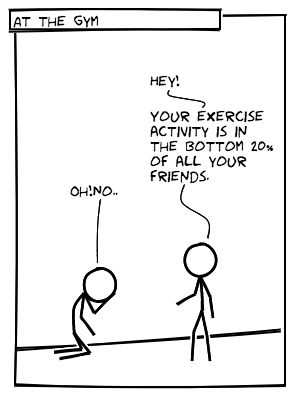
\includegraphics[width=0.21\textwidth]{figures/intro_new.png}
  \vspace{-10pt}
  \caption{An example single comic panel in abstract comic form.} \label{fig:intro}
  \vspace{-10pt}
\end{wrapfigure}

Despite the importance of the comic form in contemporary culture, and the use of the comic form in educational settings, there is surprisingly limited work examining the effects of the comic form to stimulate behavior. In particular, we focus on the use of an abstract comic form. By an abstract representation, (see~\Cref{fig:intro} for an example) we mean that the comic de-emphasizes character detail (face, eyes, etc.) or details about the locale. As~\textcite{scott1993understanding} points out, using abstract representations for the comic allows the reader to project themselves onto the comic character. The abstract form has an additional benefit: since the form is visually spare, it allows for comic panel algorithmic synthesis and for the personalization of messages. In this paper, we used a three-panel comic in abstract form.

We use an online charitable donation task for our experiment: the task is a  single-shot task, contributes to the public good with distant, non-exclusive rewards, occurs frequently, and easily tested for at scale. We chose a charity associated with Autism (Organization for Autism Research) for our experiment.

Thus, in this work we answer two research questions in the context of the online charitable donation task:
\begin{description}
    \item[RQ1:] Does the use of the abstract comic form increase the level of donation over the plain text message? \footnote{The abstract comic includes the same text from the plain text condition. Thus both conditions indicate the same expected utility.}
    \item[RQ2:] What is the effect of introducing a social proof in the abstract comic, when compared to the comic without the social proof?
\end{description}

We would like to emphasize that it is unclear at the outset if a message in comic form ought to make any difference towards a charitable donation. An argument in favor is that comics communicate affect well and are an important element of our visual culture; an argument against is that from rational actor theory in classical Economics, since the comic includes the text message used in the text-only condition and thus cannot alter the expected utility, the comic ought to serve as an irrelevant factor. To the best of our knowledge, this is the first study to examine the persuasive power of an abstract comic in an online public good setting with distant and non-exclusive rewards. 

We ran the experiment using Amazon Mechanical Turk ($n=307$; we paid each participant above minimum wage, at \$10.0/hr) where we randomly assigned each participant to one of the three conditions ('a plain text message', 'abstract comic', 'abstract comic with social proof'). The two comic conditions include the text used in the plain text condition. The social proof case adds one additional phrase to the comic that reveals the norm.

We performed a careful Bayesian analysis to analyze the data. We agree with the observations by~\textcite{Kay2016}, that beyond the impact on experimental replicability, shifting the question from ``did it have an effect?'' to ``how strong was the effect?'' is important to the HCI community. Two additional ideas---transparency, impact small-$n$ studies---motivate our use of Bayesian analysis. First, with a Bayesian model, the researcher foregrounds all the aspects of the model; there are no modeling assumptions that need checking, not already foregrounded in the model description. Thus the model and the results are amenable to further scrutiny. Second, a Bayesian model is valid at \textit{every} value of $n$ (the number of observations); we do not have to wait for $n\geq 30$ to satisfy assumptions of Normality. For small $n$ values, the result is of course affected by the choice of the prior; but by using weakly informative priors, we can ensure that the prior doesn't dominate inference. In a sense, as ~\textcite[][Chapter 9]{McElreath2015} mentioned, Bayesian models make the \textit{most conservative} inference given the data.


\textbf{Our findings:} We show that using the comic has a significant increase in donations over the plain text conditions, with a medium to large effect size of $0.59$. Thus we can answer \textbf{RQ1} affirmatively. To answer \textbf{RQ2}, we show that while the comic with social proof increases the donation level over the comic without the norm, the effect size is very small ($0.11$) and the increase is not significant. To summarize, the comic form significantly increases donations over the plain text, but the presence of the social proof is not effective. We caution that the result holds for single-shot, public goods tasks. To fully understand the value of incorporating the social proof in the comic, for specific longitudinal tasks such as dieting, with distant, exclusive rewards and where habits can confound, we need future research.  

\textbf{Design Implications:} The primary design implication of our findings: helping non-profits and governmental agencies with their online messaging strategies as they work to alleviate public goods dilemmas. In particular, public-goods dilemmas that require single-shot decisions (online charitable donations) are opportune candidates for intervention. We believe that these agencies can easily include the use of the comic form as part of their overall messaging strategy because the simplicity of the abstract comic form allows it to be easily synthesized (as we discuss in~\Cref{sub:framework}, towards of the end of this paper) and to additionally incorporate social proofs. 


The rest of this paper is organized as follows. In the next section, we discuss related work.~\Cref{sec:relatedwork} introduces two motivating ideas: the abstract comic form, and the idea of the social proof.~\Cref{sec:Method} introduces our experimental method and in~\Cref{sec:Study on Behavior Results} we present our Bayesian analysis. In~\Cref{sec:Model Criticism}, we analyze the model for convergence and also discuss alternative models.~\Cref{sec:Discussion} summarizes the main findings, discusses how we could algorithmically synthesize the comic panels and then identifies limitations. We present our conclusions in~\Cref{sec:Conclusion}. 

% %!TEX root = cscw2019-comic.tex

% what is the problem?

% why is it important? what is the impact? what motivates?

% who else has done it?
% what did you do?

\section{introduction}
\label{sec:introduction}

\begin{wrapfigure}{R}{0.23\textwidth}
    \centering
    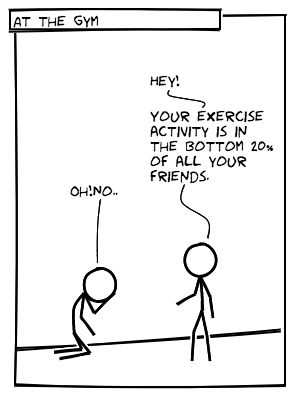
\includegraphics[width=0.21\textwidth]{figures/intro_new.png}
  \vspace{-10pt}
  \caption{The use of an abstract comic form.} \label{fig:intro}
  \vspace{-10pt}
\end{wrapfigure}

%From engaging collective action participation to individual health tracking, persuasion play an important role in nudging people to take the action.
Are text messages (e.g. ``"Would you like to donate to support the Organization for Autism Research?"'') more persuasive when expressed in comic\footnote{We use ``comic form'' as opposed to the more formal ``graphic form'' to avoid any confusion with other visual representations of data, including charts and diagrams.} form? Embellishing a text message using a comic form appears to be a ``Supposedly Irrelevant Factor''~\cite{Thaler2015}, that ought to make no difference to a decision maker since the comic offers no additional information.

The notion of behavior change motivates us to address this question. As the quantified self movement~\cite{Epstein2014,Choe2014} illustrates, people have an enduring sense of curiosity about their lives, and develop different processes to instrument (e.g. using a wearable device) and to reflect on data gathered about their activities. Individuals use this information (``checked in at the gym twice this week''), to take decisions to change behavior (e.g. ``exercise more''; ``eat healthy'').In macro-scale collective action dilemmas, individual contributions to the dilemma (e.g. ``by traveling to Boston from Los Angeles on a plane, you generate 20\% of the greenhouse gases that your car emits each year'') are often presented as statistical facts.While visualizations often accompany these messages ( e.g. a graph of weight over time for a person interested in weight loss), the message itself is presented in textual form.

Human beings show significant resistance to changing their behavior. While there may be confounds that explain away poor adoption, including, message timing~\cite{Fogg2009} (i.e. when we show the fact), time scarcity~\cite{Janssen2016} (i.e. we don't have time to digest the information), viewing messages on smartphones~\cite{Kim2016} (screen is too small to communicate effective visualizations), rethinking the textual form of the message for easier consumption in the context of behavior change has been largely unexplored.  
 
Comic is a sophisticated form of art~\cite{scott1993understanding} that popular across cultures allowing for use of humor and affects in communication. Effectively communicating emotion and affects is key to capture reader's attention which opens the very first step for successful persuasion. In this study, we focus on abstract comic representations (see~\Cref{fig:intro}). By an abstract representation, we mean that the comic de-emphasizes character detail (face, eyes etc.), or details about the locale. As~\textcite{scott1993understanding} points out, using abstract representations for the comic allows the reader to project themselves onto the comic character which may make the persuadee less resistant to receive and digest the message. Equally importantly, if we wish to algorithmically synthesize comic-style messages, abstract representations allow for a straightforward synthesis and for use in a wide variety of contexts. Furthermore, comics are usually in the form of juxtaposed sequences of panels of images or a standalone single image. Besides the graphical representation, textual elements such as speech balloons, captions, and onomatopoeia often communicate dialogue, narration, sound effects, or other information. Existing work shows that comics can effectively convey meanings \cite{McDermottPB18,cary2004going,scott1993understanding}.

In this study, we explored a novel way to present persuasive messages, ''abstract comic'' . We compared the persuasive power of the same message (e.g. "Would you like to donate to support the Organization for Autism Research?") in two different forms, pure-textual and abstract comic, that aim to persuade individuals to make charitable donation decisions. Then we tested the use of social proof, one of the most widely used persuasive techniques, in abstract comic persuasion. 

Although persuasive messages are widely used to appeal for different causes for example exercise and environment protection, in this study. we tested the persuasiveness of abstract comic messages in persuading people to make charitable donations. We believe there are three key aspects we need to pay attention when selecting the persuasive task to test the persuasive power of abstract comic messages. First of all, the persuasive task should be ecologically valid. Testing the persuasive power on a hypothetical goal may hurt the generalizability of the result. With the advance in technology and social network, more and more charities or non-profit organizations solicit donation online. However, asking for charitable giving is hard. According to Wikipedia's fundraising report, the conversion rate is only 0.3 \%. So online charitable donation is a real and difficult task for persuasion. Second, we believe to effectively test the persuasiveness the persuasive goal should be soliciting the voluntary donation of tangible resources such as time, money, or effort. Any external rewards may confound our study design as people may have different utility towards them. In charitable donation scenario, people's decision is completely voluntary and people will receive no external rewards. Also, people need to contribute their money when decide to donate. Third, the persuasion outcome should be easy to measure. For example, comparing to the exercise outcome, the amount of money people are willing to donate for charitable causes is easier and more straightforward to measure. Therefore, in this study, we tested the persuasiveness of abstract comic messages in encouraging people to make charitable donation decisions on public health research. 

In this study, we ask,
\begin{description}
 \item[RQ-1]: Are text messages more persuasive when expressed in abstract comic form when encouraging individuals to contribute to public goods?
 \item[RQ-2]: What is the effect of 'social proof' in modulating comic persuasiveness?
\end{description} 

To answer the above questions, we conducted a persuasion study ($n=307$) on Amazon Mechanical Turk (after IRB approval). We examined if participants are persuaded to donate to a charity when presented with a three-panel abstract comic; we also performed an additional experiment that combined the idea of the social proof with the comic message.

We analyzed the results using a hierarchical Bayesian framework. Consistent with the observations by~\textcite{Kay2016}, we believe that beyond the role of Bayesian analysis on the issue of replicability, by shifting the question from the binary ``did it have an effect?'' to ``how strong is the effect?'' is important in small-$n$ studies common to HCI.

Our contributions are two-fold: First, we show through our study that the abstract comic form is more persuasive than the corresponding text message. The effect ($0.59$) is of medium size and meaningful. The use of social proof improves the persuasiveness of the comic, but the effect size is minor ($0.11$) and not meaningful. Second, based on our study result, we proposed a general framework that can easily synthesis textual persuasive messages into abstract comic forms. 

We organize the rest of this paper as follows: we first present related work and motivating ideas. Then, we present our study design and result. Then, we discuss the implications of our results, including study limitations, followed by conclusions.

% we tested the persuasiveness of abstract messages in charitable donation decisions.
% To test the persuasiveness of abstr


% While those persuasive techniques have made persuasive messages appeal more, human beings show significant resistance to cooperate in collective actions and contribute to public goods. Although there may be confounds that explain away poor adoption, including, message timing~\cite{Fogg2009} (i.e. when we deliver the message), time scarcity~\cite{Janssen2016} (i.e. we don't have time to digest the information), viewing messages on smartphones~\cite{Kim2016} (screen is too small to communicate effective visualizations), rethinking the textual form of the message for easier consumption in the context of behavior change has been largely unexplored.

% In this study, we explored a novel way to present persuasive messages, ''abstract comic'' \footnote{We use ``comic form'' as opposed to the more formal ``graphic form'' to avoid any confusion with other visual representations of data, including charts and diagrams.}. We compared the persuasive power of the same message (e.g. "Would you like to donate to support the Organization for Autism Research?") in two different forms, pure-textual and abstract comic, that aim to encourage individuals to contribute to the public goods (e.g. making online charitable donation decisions). Then we tested the use of social proof, one of the most widely used persuasive techniques, in abstract comic persuasion. 



% Three ideas underpin this paper: information framing, ``social proof,'' and the comic form. First, work in Behavioral Economics~\cite{tversky1992advances,tversky1981framing} shows that how we frame the text matters and can cause preference reversal. Briefly, individuals show different preferences to statements with identical information due to risk aversion.
%  (e.g. ``if you take the plane, there is a 50\% chance that you will fall ill'' vs. ``if you take the plane there is a 50\% chance that you will be healthy''; the former is more salient due to risk aversion). We plan to use frames to represent statistical facts.
%  Second, work in Psychology shows that individuals' decisions are guided by social norms~\cite{goldstein2008room,schultz2007constructive}.
%  In a well known experiment on the design of signs for towel reuse,~\textcite{goldstein2008room} showed that use of social norms in the message had a significant impact on towel re-use, when compared to the standard sign that asks us to re-use towels to save water. In a related study,~\textcite{schultz2007constructive} demonstrated the positive impact of comparing one's energy consumption patterns with that of one's neighbors. Today, many households in the U.S. receive bills from their utility companies comparing their energy use to their neighbors as a consequence of this study. In our paper, we use this idea of the ``social proof'', by comparing the performance of an individual to that of her friends.
%  Finally, we use comics in abstract form to communicate. Comics is a sophisticated form of art~\cite{scott1993understanding} that popular across cultures allowing for use of humor and affect in communication. We focus on abstract comic representations (see~\Cref{fig:intro}). By an abstract representation, we mean that the comic de-emphasizes character detail (face, eyes etc.), or details about the locale. As~\textcite{scott1993understanding} points out, using abstract representations for the comic allows the reader to project themselves onto the comic character.
%  Equally importantly, if we wish to algorithmically synthesize comic-style messages, abstract representations allows for a straightforward synthesis and for use in a wide variety of contexts.
% While the comic form has found use in scientific communication~\cite{McDermottPB18} and in a multilingual classroom~\cite{cary2004going}, its use in behavior change is not yet well understood.

% one of the most popular form of art across different cultures.


% Comics are usually in the form of juxtaposed sequences of panels of images or a standalone single image. Beside the graphical representation, textual elements such as speech balloons, captions, and onomatopoeia often communicate dialogue, narration, sound effects, or other information. Existing work shows that comics can effectively convey meanings \cite{McDermottPB18,cary2004going,scott1993understanding}. Yet the persuasiveness of the comics representation has not been investigated.


% Hotel guests start to reuse their towels more because of a subtle change of a sign positioned on washroom towel racks \cite{goldstein2008room}. Households start to reduce their energy consumption because of an emoji on their energy bill \cite{schultz2007constructive}.






% % Today, the world generates information all around us every second. We are surrounded by all sorts of messages trying to change what we think and what we do: our newsfeed is full of advertisements, our wearable devices are keeping telling us to exercise more, even our water bottle starts to push notification to remind us stay hydrated. However, not all messages can successfully make us change: we won't buy an expensive car because of a short video, we often eat junk food even though we received a lot of articles about health eating and we are often in the status of dehydration after reading those notifications. Thus, how to make a message more persuasive has been a critical problem throughout the years.\par

% While classical game theory suggests that recasting an informative message through a different form cannot increase the message's persuasive power, a rich body of research has demonstrated how susceptible we are to those fancy words \cite{tversky1992advances,tversky1981framing,goldstein2008room,schultz2007constructive}.

% Hotel guests start to reuse their towels more because of a subtle change of a sign positioned on washroom towel racks \cite{goldstein2008room}. Households start to reduce their energy consumption because of an emoji on their energy bill \cite{schultz2007constructive}.

% People are more willing to sign up for a prosocial peer-to-peer service because of a message on the sign-up page telling them explicitly what benefit they might get \cite{vaish2018s}. Given the susceptible nature of our species, we believe changing the representation of a message can make the message more persuasive.\par


% Comics, a medium to express ideas in a graphical form, are one of the most popular form of art across different cultures. The history of comics can be traced back to early precursors such as Trajan's Column \cite{o1971art}. Comics are usually in the form of juxtaposed sequences of panels of images or a standalone single image. Beside the graphical representation, textual elements such as speech balloons, captions, and onomatopoeia often communicate dialogue, narration, sound effects, or other information. Existing work shows that comics can effectively convey meanings \cite{McDermottPB18,cary2004going,scott1993understanding}. Yet the persuasiveness of the comics representation has not been investigated.


% In this study, we want to answer the following research questions related to communication of statistical facts.

% \begin{description}
%  \item[RQ-1]: Are statistical facts about individual behavior more persuasive when presented through abstract comic form?
%  \item [RQ-2]: What the effect of the elements of the comic form, specifically gesture, shading and distance between characters, in modulating comic persuasiveness?
%  \item [RQ-3]: What is the effect of information framing in modulating comic persuasiveness?
%  \item [RQ-4]: Can we algorithmically synthesize abstract comics for communicating statistical facts?
% \end{description}

% To examine the question if the abstract comic form is more persuasive than the corresponding text message, we employed an iterative design framework and conducted two studies (after IRB approval) on Amazon Mechanical Turk. 

% In the first study ($n=146$) we examined if the comic form is preferred over text. We manipulated character gesture (3 cases), distance between characters (3 cases), shading (3 cases) and framing (2 cases), giving us a total of 54 conditions. In the second study on persuasion ($n=307$), we examined if participants are persuaded to donate to a charity when presented with a three panel comic; we also performed an additional experiment that combined the idea of the social proof with the comic message.

% We analyzed the results of both studies using a hierarchical Bayesian framework. Consistent with the observations by~\textcite{Kay2016}, we believe that beyond the role of Bayesian analysis on the issue of replicability, by shifting the question from the binary ``did it have an effect?'' to ``how strong is the effect?'' is important in small-$n$ studies common to HCI.

% We show through our study that the abstract comic form is more persuasive that the corresponding text message. The effect (0.48) is of medium size and significant. The use of the social proof improves the persuasiveness of the comic, but the effect size is minor (0.12) and not meaningful.

% Our contributions are as follows:
% \begin{description}
%   \item[Preference study:] We show through our first study that the comic form is preferred over the text message. The effect size (0.32) is moderate, but significant. Our further analysis shows that while information framing improves the preference of the comic, the effect is minor and not significant. Similarly, gesture, inter-character distance, and shading all have minor, not significant effects.
%   \item[Persuasion study:] 
% \end{description}

% Our findings have several design implications. First, we could consider using an abstract comic form to communicate messages for behavior change (e.g. wearable devices). Second, abstract comic form messages can be algorithmically synthesized, by mapping the frame type (positive or negative) to the character gesture, and the statistical information may be obtained from a person's history and from behavioral data of friends who have agreed to share.

% The code for Bayesian analysis, comic generator and the raw data will be released under an appropriate open source license.


% Our findings show that comics are more persuasive than text, with a moderate effect size of 0.33. We see strong influence for gestures and shadings that are not neutral, and moderate influence when distance between characters is large. Negatively framed messages have a stronger influence than do positively framed messages. We performed an additional small scale study on Mechanical Turk, to understand the role of color, since comic strips found in newspapers (and XKCD) infrequently use color. Our findings are that the choice of color and which element to color (text, character or background line) matters, but we need a larger study to develop a nuanced understanding of interaction effects between color and the other comic elements.

% To summarize: our main contributions lie in analyzing the effect of abstract comics in communicating statistical facts, including the effects of the different comic elements. We developed an algorithmic framework to synthesize the comic panels.
% We plan to release the code for Bayesian analysis, comic generator and the raw data under an appropriate open source license.



%From donation solicitation email to online fund-raising campaign, technology advancement expands ways for people to contribute for charitable causes. Research has shown that contributing to public goods such as charitable fund is essential to social prosperity ~\cite{marwell1981economists,marwell1979experiments,isaac1982public}. Without individuals' contribution, some public goods such as charitable fund may become scarce. However, since public goods cannot be confined solely to those who have paid for it, there is no tangible utility for people to contribute ~\cite{marwell1981economists,marwell1979experiments,isaac1982public}. Therefore, extensive efforts had been put to understand how to make individuals act in such collective action dilemma.

%Although free-riders exist in collective actions, people vote, volunteer time, donate to charitable organizations, and even risk their life for strangers. Intrinsic motives such as altruism ~\cite{olson2009logic,andreoni1990impure}, sympathy~\cite{becker1974theory}, and self-esteem ~\cite{burnett1981psychographic} drive people to contribute to public goods. Meanwhile, when people making decisions on devoting their money, time, and efforts to public goods, there were factors from outside world influencing other than pure good faith. Nudges from the organization or the government are one of the most influential factors. Those nudges are often simple (pure textual-form) and framed to persuade people for a specific cause. Although those persuasive messages look very simple, their persuasive power should not be underestimated. For example, Wikipedia, the world's largest free encyclopedia written by volunteers, raised over 30 million funds in 2016-2017 through a text banner on the top of each article \cite{wikimediafoundation}. 

%To further equip messages with adequate persuasive power, persuasion researchers found human often take heuristics when making decisions and those heuristics can be exploited by adversaries as the bait to lure an individual into behavior that counters to his/her best interests. ~\textcite{cialdini2007influence} called those baits as psychological principles of influence. Studies concluded seven principles including, authority, commitment, liking, perceptual contrast, reciprocation, scarcity, and social proof. With such influence weapons, persuader can easily frame the original messages in a different way that can be perceived as more convincing. For example, in a well-known experiment on the design of signs for towel reuse,~\textcite{goldstein2008room} showed that use of social proof in the message had a significant impact on towel re-use when compared to the standard sign that asks us to re-use towels to save water. 

%While those persuasive techniques have made persuasive messages appeal more, human beings show significant resistance to cooperate in collective actions and contribute to public goods. Although there may be confounds that explain away poor adoption, including, message timing~\cite{Fogg2009} (i.e. when we deliver the message), time scarcity~\cite{Janssen2016} (i.e. we don't have time to digest the information), viewing messages on smartphones~\cite{Kim2016} (screen is too small to communicate effective visualizations), rethinking the textual form of the message for easier consumption in the context of behavior change has been largely unexplored.

%In this study, we explored a novel way to present persuasive messages, ''abstract comic'' \footnote{We use ``comic form'' as opposed to the more formal ``graphic form'' to avoid any confusion with other visual representations of data, including charts and diagrams.}. We compared the persuasive power of the same message (e.g. "Would you like to donate to support the Organization for Autism Research?") in two different forms, pure-textual and abstract comic, that aim to encourage individuals to contribute to the public goods (e.g. making online charitable donation decisions). Then we tested the use of social proof, one of the most widely used persuasive techniques, in abstract comic persuasion. 
 
%Two ideas underpin this paper: the abstract comic form and the idea of social proof. First, comic is a sophisticated form of art~\cite{scott1993understanding} that popular across cultures allowing for use of humor and affects in communication. Effectively communicating emotion and affects is key to capture reader's attention which opens the very first step for successful persuasion. In this study, we focus on abstract comic representations (see~\Cref{fig:intro}). By an abstract representation, we mean that the comic de-emphasizes character detail (face, eyes etc.), or details about the locale. As~\textcite{scott1993understanding} points out, using abstract representations for the comic allows the reader to project themselves onto the comic character which may make the persuadee less resistant to receive and digest the message. Equally importantly, if we wish to algorithmically synthesize comic-style messages, abstract representations allow for a straightforward synthesis and for use in a wide variety of contexts. Furthermore, comics are usually in the form of juxtaposed sequences of panels of images or a standalone single image. Besides the graphical representation, textual elements such as speech balloons, captions, and onomatopoeia often communicate dialogue, narration, sound effects, or other information. Existing work shows that comics can effectively convey meanings \cite{McDermottPB18,cary2004going,scott1993understanding}. Second, work in Behavioral Economics~\textcite{tversky1992advances,tversky1981framing} and Psychology \cite{cialdini2007influence} shows that simply states the goal of persuasion is not enough. Framing the message with ''influence weapons'' is crucial. Since comics have the ability to tell a great story, it is reasonable to believe persuasive messages in abstract comic form can also adapt those weapons of influence to appeal.  

%However embellishing a text message using a comic form appears to be a ``Supposedly Irrelevant Factor''~\cite{Thaler2015}, that ought to make no difference to a decision maker since the comic offers no additional information. Therefore in this study, we ask,
% %\begin{description}
%  \item[RQ-1]: Are text messages more persuasive when expressed in abstract comic form when encouarging individuals to contribute to public goods?
%  \item[RQ-2]: What is the effect of 'social proof' in modulating comic persuasiveness?
% \end{description} 

%To answer the above questions, we conducted a persuasion study ($n=307$) on Amazon Mechanical Turk (after IRB approval). We examined if participants are persuaded to donate to a charity when presented with a three-panel abstract comic; we also performed an additional experiment that combined the idea of the social proof with the comic message.

%We analyzed the results using a hierarchical Bayesian framework. Consistent with the observations by~\textcite{Kay2016}, we believe that beyond the role of Bayesian analysis on the issue of replicability, by shifting the question from the binary ``did it have an effect?'' to ``how strong is the effect?'' is important in small-$n$ studies common to HCI.

%Our contributions are two-fold: First, we show through our study that the abstract comic form is more persuasive than the corresponding text message. The effect ($0.44$) is of medium size and meaningful. The use of social proof improves the persuasiveness of the comic, but the effect size is minor ($0.11$) and not meaningful. Second, based on our study result, we proposed a general framework that can easily synthesis textual persuasive messages into abstract comic forms. 

%We organize the rest of this paper as follows: we first present related work and motivating ideas. Then, we present our study design and result. Then, we discuss the implications of our results, including study limitations, followed by conclusions.


%First, work in Behavioral Economics~\cite{tversky1992advances,tversky1981framing} shows that how we frame the text matters and can cause preference reversal. Briefly, individuals show different preferences to statements with identical information due to risk aversion.
% (e.g. ``if you take the plane, there is a 50\% chance that you will fall ill'' vs. ``if you take the plane there is a 50\% chance that you will be healthy''; the former is more salient due to risk aversion). We plan to use frames to represent statistical facts.
 %Second, work in Psychology shows that individuals' decisions are guided by social norms~\cite{goldstein2008room,schultz2007constructive}.
%  In a well known experiment on the design of signs for towel reuse,~\textcite{goldstein2008room} showed that use of social norms in the message had a significant impact on towel re-use, when compared to the standard sign that asks us to re-use towels to save water. In a related study,~\textcite{schultz2007constructive} demonstrated the positive impact of comparing one's energy consumption patterns with that of one's neighbors. Today, many households in the U.S. receive bills from their utility companies comparing their energy use to their neighbors as a consequence of this study. In our paper, we use this idea of the ``social proof'', by comparing the performance of an individual to that of her friends.
 %Finally, we use comics in abstract form to communicate. Comics is a sophisticated form of art~\cite{scott1993understanding} that popular across cultures allowing for use of humor and affect in communication. We focus on abstract comic representations (see~\Cref{fig:intro}). By an abstract representation, we mean that the comic de-emphasizes character detail (face, eyes etc.), or details about the locale. As~\textcite{scott1993understanding} points out, using abstract representations for the comic allows the reader to project themselves onto the comic character.
 %Equally importantly, if we wish to algorithmically synthesize comic-style messages, abstract representations allows for a straightforward synthesis and for use in a wide variety of contexts.



%Are text messages (e.g. ``you've exercised 25\% more than you did last week'') more persuasive when expressed in comic\footnote{We use ``comic form'' as opposed to the more formal ``graphic form'' to avoid any confusion with other visual representations of data, including charts and diagrams.} form? Embellishing a text message using a comic form appears to be a ``Supposedly Irrelevant Factor''~\cite{Thaler2015}, that ought to make no difference to a decision maker since the comic offers no additional information.

%The notion of behavior change motivates us to address this question. As the quantified self movement~\cite{Epstein2014,Choe2014} illustrates, people have an enduring sense of curiosity about their lives, and develop different processes to instrument (e.g. using a wearable device) and to reflect on data gathered about their activities. Individuals use this information (``checked in at the gym twice this week''), to take decisions to change behavior (e.g. ``exercise more''; ``eat healthy'').
% In macro-scale collective action dilemmas, individual contributions to the dilemma (e.g. ``by traveling to Boston from Los Angeles on a plane, you generate 20\% of the greenhouse gases that your car emits each year'') are often presented as statistical facts.
 %While visualizations often accompany these messages ( e.g. a graph of weight over time for a person interested in weight loss), the message itself is presented in textual form.

%Human beings show significant resistance to changing their behavior. While there may be confounds that explain away poor adoption, including, message timing~\cite{Fogg2009} (i.e. when we show the fact), time scarcity~\cite{Janssen2016} (i.e. we don't have time to digest the information), viewing messages on smartphones~\cite{Kim2016} (screen is too small to communicate effective visualizations), rethinking the textual form of the message for easier consumption in the context of behavior change has been largely unexplored.

%Three ideas underpin this paper: information framing, ``social proof,'' and the comic form. First, work in Behavioral Economics~\cite{tversky1992advances,tversky1981framing} shows that how we frame the text matters and can cause preference reversal. Briefly, individuals show different preferences to statements with identical information due to risk aversion.
%  (e.g. ``if you take the plane, there is a 50\% chance that you will fall ill'' vs. ``if you take the plane there is a 50\% chance that you will be healthy''; the former is more salient due to risk aversion). We plan to use frames to represent statistical facts.
 %Second, work in Psychology shows that individuals' decisions are guided by social norms~\cite{goldstein2008room,schultz2007constructive}.
%  In a well known experiment on the design of signs for towel reuse,~\textcite{goldstein2008room} showed that use of social norms in the message had a significant impact on towel re-use, when compared to the standard sign that asks us to re-use towels to save water. In a related study,~\textcite{schultz2007constructive} demonstrated the positive impact of comparing one's energy consumption patterns with that of one's neighbors. Today, many households in the U.S. receive bills from their utility companies comparing their energy use to their neighbors as a consequence of this study. In our paper, we use this idea of the ``social proof'', by comparing the performance of an individual to that of her friends.
 %Finally, we use comics in abstract form to communicate. Comics is a sophisticated form of art~\cite{scott1993understanding} that popular across cultures allowing for use of humor and affect in communication. We focus on abstract comic representations (see~\Cref{fig:intro}). By an abstract representation, we mean that the comic de-emphasizes character detail (face, eyes etc.), or details about the locale. As~\textcite{scott1993understanding} points out, using abstract representations for the comic allows the reader to project themselves onto the comic character.
 %Equally importantly, if we wish to algorithmically synthesize comic-style messages, abstract representations allows for a straightforward synthesis and for use in a wide variety of contexts.
%While the comic form has found use in scientific communication~\cite{McDermottPB18} and in a multilingual classroom~\cite{cary2004going}, its use in behavior change is not yet well understood.

% one of the most popular form of art across different cultures.
%
%
% Comics are usually in the form of juxtaposed sequences of panels of images or a standalone single image. Beside the graphical representation, textual elements such as speech balloons, captions, and onomatopoeia often communicate dialogue, narration, sound effects, or other information. Existing work shows that comics can effectively convey meanings \cite{McDermottPB18,cary2004going,scott1993understanding}. Yet the persuasiveness of the comics representation has not been investigated.


% Hotel guests start to reuse their towels more because of a subtle change of a sign positioned on washroom towel racks \cite{goldstein2008room}. Households start to reduce their energy consumption because of an emoji on their energy bill \cite{schultz2007constructive}.






% Today, the world generates information all around us every second. We are surrounded by all sorts of messages trying to change what we think and what we do: our newsfeed is full of advertisements, our wearable devices are keeping telling us to exercise more, even our water bottle starts to push notification to remind us stay hydrated. However, not all messages can successfully make us change: we won't buy an expensive car because of a short video, we often eat junk food even though we received a lot of articles about health eating and we are often in the status of dehydration after reading those notifications. Thus, how to make a message more persuasive has been a critical problem throughout the years.\par

% While classical game theory suggests that recasting an informative message through a different form cannot increase the message's persuasive power, a rich body of research has demonstrated how susceptible we are to those fancy words \cite{tversky1992advances,tversky1981framing,goldstein2008room,schultz2007constructive}.
%
% Hotel guests start to reuse their towels more because of a subtle change of a sign positioned on washroom towel racks \cite{goldstein2008room}. Households start to reduce their energy consumption because of an emoji on their energy bill \cite{schultz2007constructive}.

% People are more willing to sign up for a prosocial peer-to-peer service because of a message on the sign-up page telling them explicitly what benefit they might get \cite{vaish2018s}. Given the susceptible nature of our species, we believe changing the representation of a message can make the message more persuasive.\par


% Comics, a medium to express ideas in a graphical form, are one of the most popular form of art across different cultures. The history of comics can be traced back to early precursors such as Trajan's Column \cite{o1971art}. Comics are usually in the form of juxtaposed sequences of panels of images or a standalone single image. Beside the graphical representation, textual elements such as speech balloons, captions, and onomatopoeia often communicate dialogue, narration, sound effects, or other information. Existing work shows that comics can effectively convey meanings \cite{McDermottPB18,cary2004going,scott1993understanding}. Yet the persuasiveness of the comics representation has not been investigated.


% In this study, we want to answer the following research questions related to communication of statistical facts.

% \begin{description}
%  \item[RQ-1]: Are statistical facts about individual behavior more persuasive when presented through abstract comic form?
%  \item [RQ-2]: What the effect of the elements of the comic form, specifically gesture, shading and distance between characters, in modulating comic persuasiveness?
%  \item [RQ-3]: What is the effect of information framing in modulating comic persuasiveness?
%  \item [RQ-4]: Can we algorithmically synthesize abstract comics for communicating statistical facts?
% \end{description}

%To examine the question if the abstract comic form is more persuasive than the corresponding text message, we employed an iterative design framework and conducted two studies (after IRB approval) on Amazon Mechanical Turk. 

%In the first study ($n=146$) we examined if the comic form is preferred over text. We manipulated character gesture (3 cases), distance between characters (3 cases), shading (3 cases) and framing (2 cases), giving us a total of 54 conditions. In the second study on persuasion ($n=307$), we examined if participants are persuaded to donate to a charity when presented with a three panel comic; we also performed an additional experiment that combined the idea of the social proof with the comic message.

%We analyzed the results of both studies using a hierarchical Bayesian framework. Consistent with the observations by~\textcite{Kay2016}, we believe that beyond the role of Bayesian analysis on the issue of replicability, by shifting the question from the binary ``did it have an effect?'' to ``how strong is the effect?'' is important in small-$n$ studies common to HCI.

%We show through our study that the abstract comic form is more persuasive that the corresponding text message. The effect (0.48) is of medium size and significant. The use of the social proof improves the persuasiveness of the comic, but the effect size is minor (0.12) and not meaningful.

% Our contributions are as follows:
% \begin{description}
%   \item[Preference study:] We show through our first study that the comic form is preferred over the text message. The effect size (0.32) is moderate, but significant. Our further analysis shows that while information framing improves the preference of the comic, the effect is minor and not significant. Similarly, gesture, inter-character distance, and shading all have minor, not significant effects.
%   \item[Persuasion study:] 
% \end{description}

%Our findings have several design implications. First, we could consider using an abstract comic form to communicate messages for behavior change (e.g. wearable devices). Second, abstract comic form messages can be algorithmically synthesized, by mapping the frame type (positive or negative) to the character gesture, and the statistical information may be obtained from a person's history and from behavioral data of friends who have agreed to share.

% The code for Bayesian analysis, comic generator and the raw data will be released under an appropriate open source license.


% Our findings show that comics are more persuasive than text, with a moderate effect size of 0.33. We see strong influence for gestures and shadings that are not neutral, and moderate influence when distance between characters is large. Negatively framed messages have a stronger influence than do positively framed messages. We performed an additional small scale study on Mechanical Turk, to understand the role of color, since comic strips found in newspapers (and XKCD) infrequently use color. Our findings are that the choice of color and which element to color (text, character or background line) matters, but we need a larger study to develop a nuanced understanding of interaction effects between color and the other comic elements.

% To summarize: our main contributions lie in analyzing the effect of abstract comics in communicating statistical facts, including the effects of the different comic elements. We developed an algorithmic framework to synthesize the comic panels.
% We plan to release the code for Bayesian analysis, comic generator and the raw data under an appropriate open source license.


%!TEX root = cscw2019-comic.tex
\section{Related Work}
\label{sec:relatedwork}
Now, we discuss related works in: 1) Using Comics to Communicate Ideas, 2) Persuasion through Visual Stimuli, 3) Persuasion for Public Goods, and 4) Social Proof in Persuasive Messages.

\subsection{Using Comics to Communicate Ideas}
\textcite{scott1993understanding} defines comics as ``juxtaposed pictorial and other images in deliberate sequence, intended to convey information and/or to produce an aesthetic response in the viewer.`` While reading comics book is commonly recognized as entertaining, comics have been examined as an effective way of communicating abstract and complex ideas to broad audiences \cite{McDermottPB18,cary2004going,scott1993understanding, Zhang-Kennedy:2017:SCI:3206217.3206282}. On one hand, the simple and humorous nature of comic makes comics become a unique media for delivering informative and memorable messages. By combining visual elements and text, comics make the story more appealing. \textcite{McDermottPB18} used comics to illustrate complex scientific facts. In education, comics have been used and examined as a useful media for reaching populations with various backgrounds \cite{McDermottPB18,cary2004going,scott1993understanding}. \textcite{Zhang-Kennedy:2017:SCI:3206217.3206282} created ``Secure Comics`` to educate end-users on computer security knowledge. On the other hand, the use of metaphor in comics can make the underlying meaning more vivid and memorable than using a straightforward description \cite{McDermottPB18,scott1993understanding}. Moreover, comics can contain a personal story which is incredibly powerful to create empathetic feelings, a key factor in persuasion, for readers ~\cite{weaver2017losing}. ~\textcite{matsubara2016emotional} showed a link between  comic's contents and reader perceived emotions. Thus complex messages can be easily interpreted and memorized through the the comic form. Although comics has shown its strength in communicating complex and memorable ideas, its utility in persuasion has not yet been fully explored. To the best of our knowledge, we are the first study looked at abstract comics in persuading people to cooperate in collective action dilemmas.  

In our study, we chose abstract comics to persuade instead of other comic forms for the following reasons, 1) As the comic becomes more abstract, readers will be more likely to project themselves onto the character and internalizing the information the character is trying to convey \textcite{scott1993understanding}. We believe such internalization gives an extra leg when the comic is designed to persuade. 2) The simplicity requires less cognitive load from the reader to consume the message, which is ideal for persuasion since persuadee's attention is scarce \cite{Janssen2016}. 3) Comparing to other forms of the comic, the abstract comics contains least elements which lowers the cost to generate. The simplicity of abstract comics allows us to explore the idea of algorithmically synthesizing persuasive messages into the comic form. Therefore, in this study, we examined the persuasive power of messages in abstract comic form.

\subsection{Persuasion Through Visual Stimuli}
Beyond the realm of textual forms, prior research showed that using visual representations, e.g., graphics, video, and comics, are attractive in persuasion. ~\textcite{selker2015sweetbuildinggreeter} used motivational graphics or memes from 9GAG and Google to attract people's attention and persuade people for energy conservation behaviors. \textcite{consolvo2008activity} visualized user's exercise data in the Ubifit Garden to persuade people to exercise. Sometimes, the use of visual can evoke strong emotions that makes the message more persuasive. ~\textcite{iyer2006picture} found that people who saw the images of the Kenneth Bigley kidnapping were more engaged in the later civic campaign than those who read about the kidnapping from the newspaper text.\textcite{zhang2014stop}'s visual rhetoric effectively persuade users to use up-to-date antivirus protection. Visual stimuli were more memorable as well \cite{nisbett1980human}. The imaginary message makes advertisements more memorable and appealing. The visuals can leave a strong trace that can later influence people's decision making, especially when people making judgments by the availability heuristics. ~\textcite{dey2017art} found the video quality in the crowdfunding campaign plays a vital role in persuading people to support. Despite visual stimulus's benefits in persuasion, creating an effective visual persuasive message is often costly. The persuader needs to put time, effort and resource to create persuasive visual stimuli. No need to mention, thousands of considerations need to be cautious about in order to make the visual persuasive messages appealing. In our study, we looked into the abstract comic, a simple visual form that can be relatively easily created, and examined its persuasiveness in encouraging people to participate in a collective action. 
%The strong emotion carried by the photographs brought people not only fear but also engagement and concern.

\subsection{Persuasion for Public Goods}
Given the two characteristics of public goods, non-exclusive and non-rivalry, individuals will receive no tangible benefits when act in collective action dilemmas such as charitable donations ~\cite{marwell1981economists,isaac1982public}. Therefore, external nudges play an important role in encouraging people to contribute. Researchers and policymakers have extensively studied who contributes and how to persuade people to contribute ~\cite{olson2009logic,becker1974theory,andreoni1990impure,miguel2005ethnic,burnett1981psychographic,pessemier1977willingness,burnett1981psychographic}.  ~\textcite{midden2008using} reported strong persuasive power for environmental sustainable behaviors when signaling personal goals in the persuasive application. \textcite{feiler2012mixed} found emphasizing altruistic reasons in a donation request can elicit more donations from people. \textcite{mankoff2010stepgreen} successfully used social technologies to leverage public commitment and competition in appealing energy-saving behaviors. Due to the distant or non-reward nature of individuals' public goods contribution, persuasive messages were the key. Therefore, soliciting online charitable donations, a common case in collective action dilemmas, is suitable for us to test the persuasive power of abstract comics.
% when nudging people for collective actions, it is important to make the persuadee reflect upon their intrinsic motives in the messages. In our study, we believe the abstract comics allows people to project themselves onto the character which gives us the oppurtunities to nudge them to reflect upon their intrinsic motives when making decisions about cooperating in collective actions. 
%Besides education and income ~\cite{pessemier1977willingness,burnett1981psychographic}, key factors that drive people to contribute were intrinsic motives including altruism ~\cite{olson2009logic,andreoni1990impure}, sympathy ~\cite{becker1974theory}, social pressure ~\cite{miguel2005ethnic}, religiousness ~\cite{pessemier1977willingness,burnett1981psychographic} and self-esteem ~\cite{burnett1981psychographic}.

The text persuasive message is one of the most widely used methods to persuade individuals for behavior change or voluntarily charitable donations. It is easy to create and disseminate. The long history of research shows that using textual messages was effective in persuasion. ~\textcite{damgaard2017now} successfully used a simple email reminder with the decision deadline to elicit charitable donations. With a simple sign like "Turn off the tap when not in use", people reduced water consumption and engaged in energy conservation behavior change ~\cite{mckenzie2011fostering}. ~\textcite{vaish2018s} showed empathizing self-serving benefits can attract more people to sign up for a prosocial peer-to-peer service.  ~\textcite{cotterill2010impact} showed sending a pledge card with simple text "A list of everyone who donates a book will be displayed locally." encouraged 22 \% more households to donate books for Children's Book Week. However, comparing persuasive messages in other visual forms, textual messages are less effective catching perusadee's attention, especially when persudaee's attention is limited. Moreover, when it comes to memorability, one of the key measure of persuasive effect, studies found comparing to graphics and video, the text is most difficult to recall and recollect. Therefore, persuasive messages in other media such as abstract comic are worth to investigate. 


\subsection{Social Proof in Persuasive Messages }
By ``social proof,'' we refer to the idea that when individual's observation of either their friends or others they can relate adopted a behavior is persuasive for the individual to adopt the same behavior~\cite{Cialdini1993, Cialdini2004}. ``Social proof`` is widely used in encouraging individuals to cooperate in collective action dilemmas \cite{goldstein2008room,schultz2007constructive}. ~\textcite{goldstein2008room} conducted an experiment in a hotel on motivating environmental conservation. They found that descriptive norms in the persuasive message (e.g., ``the majority of guests reuse their towels'') are more persuasive than only mentioning environmental protection in the message. And the normative message got more effective when the statement is about a provincial norm (e.g., "the majority of guests in this room reuse their towels"). \textcite{amblee2011harnessing} studied ``social proof`` in online book reader communities and found that 
``electronic word of mouth `` affects book quality, author  reputation, and a book category popularity, which eventually influences people's buying decision. Since the ``social proof`` is one of the most widely used influence weapons in creating persuasive messages, we want to see if it can hold its influence power when the persuasive messages are in abstract comic form. 


%Also, we also proposed a general framework that allows the persuader to synthesize their persuasive messages into an abstract comic form easily. 




%As we presented in earlier sections, the comic allows for delivering memorable messages~\cite{scott1993understanding, Zhang-Kennedy:2017:SCI:3206217.3206282} and communicate complex ideas and emotion~\cite{McDermottPB18,cary2004going,scott1993understanding, Zhang-Kennedy:2017:SCI:3206217.3206282,weaver2017losing,matsubara2016emotional}. We believe comic is a powerful media to deliver persuasive messages.  



% \subsection{Building Persuasive Technology}
% Starting from~\textcite{goehlert1980information}, HCI researchers have spent a lot of effort in leveraging technology in persuasion.~\textcite{goehlert1980information} argues control and dissemination of information have the ability to make attitude and behavioral changes. Inspired by this argument, two approaches have been explored in constructing the persuasive systems. Information-centric approaches focused on delivering hidden or new information which has not been perceived by the user before~\cite{LeeKF11}. For example,~\textcite{chi2007enabling} changed people's nutritional composition by creating an intelligent kitchen that can provide nutritional information about ingredients while participants are cooking.  ~\textcite{liao2014expert} found showing a source expertise indicator can shape user's information seeking and burst the filter bubble. While lots of studies on persuasive technology showcase the persuasive power of the information-centric approach, studies also show the downside of information-center approach where the target receiver often failed to perceive and internalize the persuasive information ~\cite{goehlert1980information,LeeKF11}.

%Adapting decision-making models from previous behavioral research, behavior-centric approach emphasized on human motivation and biases ~\cite{LeeKF11}.~\textcite{vaish2018s} used self-serving motivational framing of messages to persuade people to join a prosocial peer-to-peer service. Although the effectiveness of behavior-centric approach has been examined in multiple studies, behavior-centric approaches often require prior knowledge of the persuadee in order to unleash the persuasion power, as~\textcite{orji2014developing} and~\textcite{schneider2016understanding} suggested that different people may be more amenable to one persuasive method than others. Therefore, due to the cost of knowing people, scalability is the key challenge.

% \subsection{Persuasion Through Visual Stimuli}
% Prior research shows that using visual representations are more attractive than text messages~\cite{selker2015sweetbuildinggreeter,consolvo2008activity}. ~\textcite{selker2015sweetbuildinggreeter} retrieves motivational images from 9GAG, Google, with energy-saving messages, to motivate people's energy saving behaviors and found those images has higher persuasive power comparing to plain text. However, images used in persuasion are costly to generate. 

% The simple and humorous nature of comic makes comics becomes an unique media for delivering informative and memorable messages. Beyond entertainment, comics can be used in scientific communication~\cite{McDermottPB18}, and for teaching in multilingual schools~\cite{cary2004going}. To the best of our knowledge, this is the first study to look at abstract comic representations and persuasion.
% The simple and humorous nature of comic makes comics becomes an unique media for delivering informative and memorable messages. While reading comics book is commonly recognized as entertaining, comics have been examined as an effective way of communicating abstract ideas to broad audiences \cite{McDermottPB18,cary2004going,scott1993understanding}. McDermott et. al used comics to illustrate complex scientific facts \cite{McDermottPB18}. In education, comics have been used and examined as an effective tool for reaching different populations with various background \cite{McDermottPB18,cary2004going,scott1993understanding}.

% Similar to images, the simple and humorous nature of comic makes comics becomes an unique media for delivering informative and memorable messages. Comics have also been examined as an effective way of communicating abstract ideas to broad audiences \cite{McDermottPB18,cary2004going,scott1993understanding}. To our knowledge, no prior study examined the persuasive power of the comic.

% We aim to fill this gap by comparing
%
% the persuasiveness between
%
% Our work aims to fill this gap by comparing the quality ofsurvey content and respondents’ engagement between theusage of a conversational survey and a traditional survey.With a few exceptions [15,16], previous work evaluatingchatbot technologies tend to rely on small-scale lab studies.Instead, we deploy a survey chatbot and study its real-worldusage of conducting marketing research survey. Our analysisis performed on the response contents and behavioral logs(e.g., time stamps), and focus on measures that are crucialfor the purpose of gathering high-quality survey data
% behavior-centric approach is scalability.
% This study mainly focuses on different comic elements' effect on persuading readers.
%
% Although persuasion can be better achieved through visual stimulus, the cost of creating personalized visual stimuli is high. Our approach leverages abstract comics taking advantage of visual stimuli while allowing for straightforward, personalized synthesis.
%
%
% Beyond entertainment, comics can be used in scientific communication~\cite{McDermottPB18}, and for teaching in multilingual schools~\cite{cary2004going}.
% The simple and humorous nature of comic makes comics becomes an unique media for delivering informative and memorable messages. While reading comics book is commonly recognized as entertaining, comics have been examined as an effective way of communicating abstract ideas to broad audiences \cite{McDermottPB18,cary2004going,scott1993understanding}. McDermott et. al used comics to illustrate complex scientific facts \cite{McDermottPB18}. In education, comics have been used and examined as an effective tool for reaching different populations with various background \cite{McDermottPB18,cary2004going,scott1993understanding}.
% The use of metaphor in comics can make the underlying meaning vivid and more memorable than using a straightforward description \cite{McDermottPB18,scott1993understanding}. Moreover, comics can contain a personal story incredibly powerful for persuasion~\cite{weaver2017losing}. With a personal story, comics can create empathy for readers.~\textcite{matsubara2016emotional} showed a link between comic's content and the emotions felt by the readers. Thus complex messages can be easily interpreted and memorized though use of the comic form.

%%!TEX root = cscw2019-comic.tex
\section{Motivating Ideas}
\label{sec:Motivating Ideas}
In this section, we present two key motivating ideas: abstract comics and social proof.

\subsection{The Abstract Comic}
As we presented in earlier sections, the comic allows for delivering memorable messages~\cite{scott1993understanding,Zhang-Kennedy:2017:SCI:3206217.3206282} and communicate complex ideas and emotion~\cite{McDermottPB18,cary2004going,scott1993understanding,Zhang-Kennedy:2017:SCI:3206217.3206282,weaver2017losing,matsubara2016emotional}. We believe comic is a powerful media to deliver persuasive messages.  

In our study, we chose abstract comics to persuade instead of other comic forms for the following reasons, 1) As the comic becomes more abstract, readers will more likely to project themselves onto the character and internalizing the information their character is trying to convey \textcite{scott1993understanding}. We believe such internalization gives an extra leg when the comic is designed to persuade. 2) Comparing to other forms of the comic, the abstract comics contains least elements which lowers the cost to generate. The also simplicity requires the reader's less cognitive load to consume the message which is ideal for persuasion since persuadee's attention is scarce. Moreover, the simplicity of abstract comics allows us to explore the idea of algorithmically synthesizing persuasive messages algorithmically into comic form. Therefore, in this study, we examined the persuasive power of abstract comics in persuading people to donate.
%Also, according to prior work when encourging people to contribute to public goods, making people reflect on their intrinsic motivation is important. The abstract the comics emphazied on 

\subsection{Social Proof}
The idea ``social proof'' is central to our study. By ``social proof,'' we refer to the idea that individuals observing either their friends or people with whom they can relate adopt a behavior, is persuasive for them to adopt the same behavior~\cite{Cialdini1993,Cialdini2004}. The use of ``social proof'' in encouraging individuals to cooperated in collective action dilemmas \cite{goldstein2008room,schultz2007constructive}. ~\textcite{goldstein2008room} conducted an influential experiment in a hotel on motivating environmental conservation. They found that descriptive norms (e.g., ``the majority of guests reuse their towels'') has more persuasive power than solely mentioning environmental protection. And this normative message gets more effective when the statement is about a provincial norm (e.g., "the majority of guests in this room reuse their towels"). Since the use of 'social proof' is one of the most widely used influence weapons in creating persuasive messages, we want to see if it can hold its influence when the persuasive messages were in the abstract comic form. 

%encouraging individuals to cooperated in collective action dilemmas. 


%environmental conservation~\textcite{goldstein2008room} and in energy conservation~\textcite{schultz2007constructive}. %Information framing refers to the idea that presenting outcomes as a gain or a loss, alters decisions~\textcite{tversky1981framing,tversky1992advances}, since individuals are loss-averse and weigh losses more severely than similar gains.


%The idea ``social proof'' (from Psychology) and ``information framing'' (from Behavioral Economics) are central to our study. By ``social proof,'' we refer to the idea that individuals observing either their friends, or people with whom they can relate adopt a behavior, is persuasive for them to adopt the same behavior~\textcite{Cialdini1993,Cialdini2004}. The use of ``social proof'' has been experimentally demonstrated in environmental conservation~\textcite{goldstein2008room} and in energy conservation~\textcite{schultz2007constructive}. Information framing refers to the idea that presenting outcomes as a gain or a loss, alters decisions~\textcite{tversky1981framing,tversky1992advances}, since individuals are loss-averse and weigh losses more severely than similar gains.
% \begin{description}
%  % \item[Memorability] Approaches to make messages more persuasive has long been a focus for a variety of different fields including computational linguistics~\cite{danescu2012you} and advertising~\cite{Bradley2002,Chamblee1993,Knapp1981,Lowrey2006}. The most simple but effective way to achieve successful and long-last persuasion is through memorability.In \cite{danescu2012you} the study showed that using unusual word choices and more general theme makes it easier to connect with reader's daily life and makes the message more memorable. Through the use of unexpected words and phrases, the message is more likely to capture reader's attention compared text using normal phrases. But the theme should be as general as possible to help readers connect with the message, so it can stay in the reader's mind longer.
%  % Ford et. al \cite{ford1991memorability} looked into the memorability of messages in organ donation and suggests less typical arguments require higher cognitive loads to process and may result in internalizing the messages into pre-existing attitude which may affect behavior.

%  \item[Social Proof]: By ``social proof,'' we refer to the idea that individuals observing either their friends, or people with whom they can relate adopt a behavior, is persuasive for them to adopt the same behavior~\cite{Cialdini1993,Cialdini2004}.~\textcite{goldstein2008room} conducted an influential experiment in a hotel on motivating environmental conservation. They found that descriptive norms (e.g., ``the majority of guests reuse their towels'') has more persuasive power than solely mentioning environmental protection. And this normative message gets more effective when the statement is about a provincial norm (e.g., "the majority of guests in this room reuse their towels"). The work by~\textcite{schultz2007constructive} also demonstrated the effectiveness of the social norm in energy conservation. In a study of 300 households in San Marcos, California, the experimenters showed residents messages that compared their energy consumption to that of their neighbors. Surprisingly, there was no change in consumption---households below the mean increased consumption, while households above the mean decreased consumption. However, when households with above average energy consumption were shown the comparison along with a `frownie' face \frownie{}, and households with below average energy consumption were shown a `smiley' face \smiley{}, both groups' energy consumption decreased. This study illustrates the power of affect, but leads to the question of utility of the comic form for communication of more sophisticated affect.
%  \item[Information Framing]: ~\textcite{tversky1981framing,tversky1992advances} found that using different reference points to frame the same sentence can result in a different response. Consider the sentences ``there is a 50\% that you will be ill if you travel by plane to New York'' and ``there is a 50\% that you will be healthy if you travel by plane to New York.'' What~\textcite{tversky1981framing} showed is that  individuals have an asymmetric utility function weighting losses more severely than similar gains. Typically a gain has be twice as large as a loss to ``cancel'' out. In general, given two prospects, individuals favor risk seeking in when confronted with sure loss, and favor risk aversion when confronted with sure gain.
% \end{description}

% Since the prior work~\cite{goldstein2008room,schultz2007constructive} suggests a robust effect of the social proof, instead of using it as part of an experimental condition, we will incorporate it in the following way: we will have two characters in the comic, shown as friends. Second, we will show comparison of the individual to a group of friends. Thus our experimental condition tests the effect of information framing in comic form:

% \textbf{RQ}: \textit{What is the effect of information framing in modulating comic persuasiveness?}

% Beyond entertainment, comics can be used in scientific communication~\cite{McDermottPB18}, and for teaching in multilingual schools~\cite{cary2004going}.
% The simple and humorous nature of comic makes comics becomes an unique media for delivering informative and memorable messages. While reading comics book is commonly recognized as entertaining, comics have been examined as an effective way of communicating abstract ideas to broad audiences \cite{McDermottPB18,cary2004going,scott1993understanding}. McDermott et. al used comics to illustrate complex scientific facts \cite{McDermottPB18}. In education, comics have been used and examined as an effective tool for reaching different populations with various background \cite{McDermottPB18,cary2004going,scott1993understanding}.
% The use of metaphor in comics can make the underlying meaning vivid and more memorable than using a straightforward description \cite{McDermottPB18,scott1993understanding}. Moreover, comics can contain a personal story incredibly powerful for persuasion~\cite{weaver2017losing}. With a personal story, comics can create empathy for readers.~\textcite{matsubara2016emotional} showed a link between comic's content and the emotions felt by the readers. Thus complex messages can be easily interpreted and memorized though use of the comic form.



% Therefore, in this study, we choose to use an abstract yet well-recognized comic style, the xkcd style created by Randall Munroe~\cite{munroe2009xkcd}, in our generated persuasive comic messages; see~\Cref{fig:xkcd}. Thus a key research question is:

% \textbf{RQ}: \textit{Are statistical facts about individual behavior more persuasive when presented through abstract comic form?}

% \begin{figure}
%  \centering
%  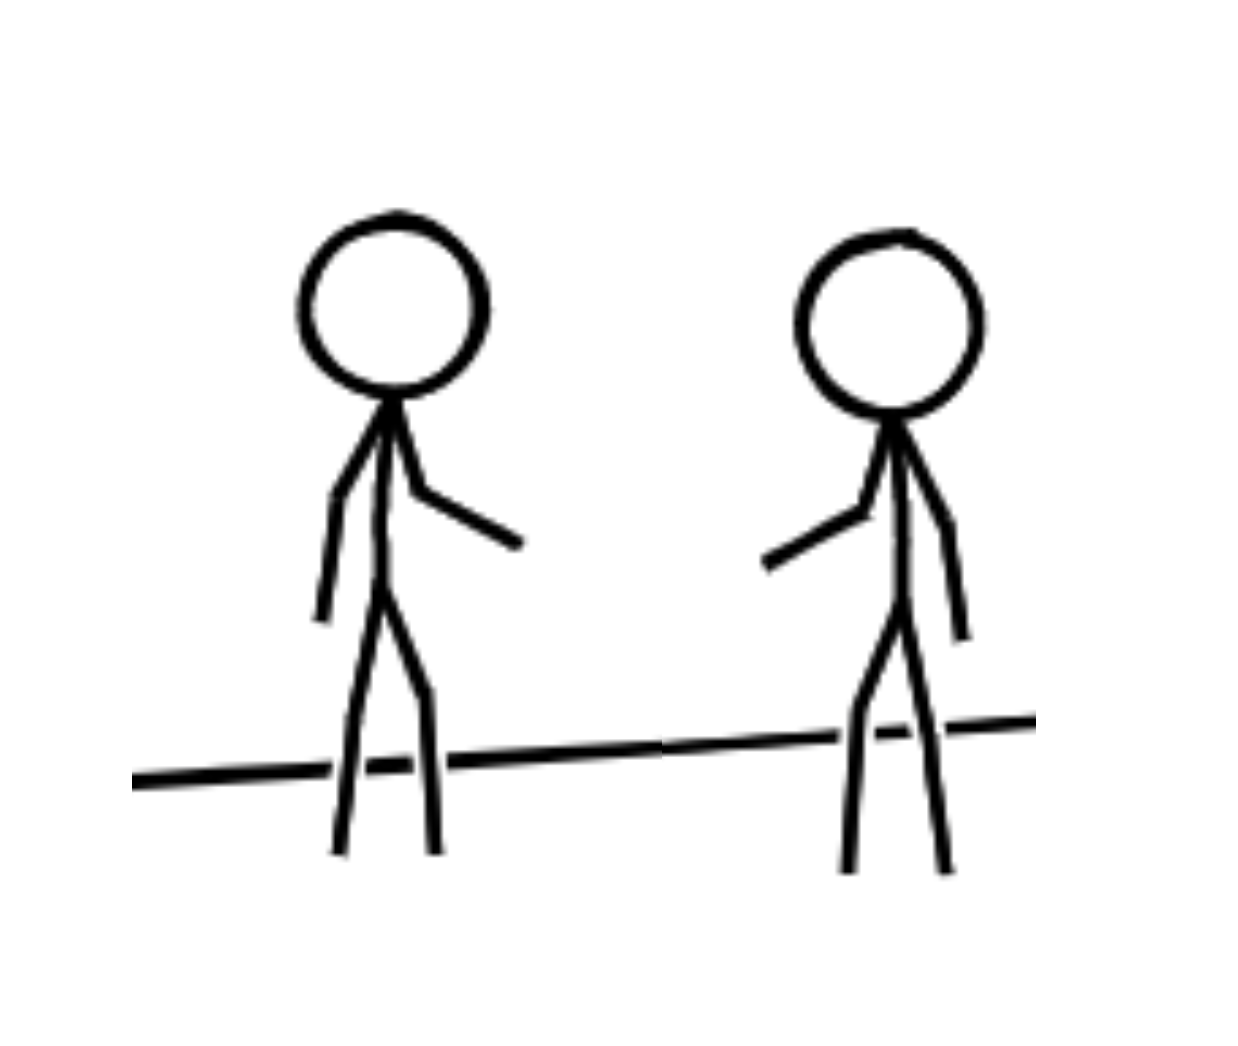
\includegraphics[width=0.3\columnwidth]{figures/xkcd_example}
%  \caption{A example of an abstract comic figure.}
%  \label{fig:xkcd}
% \end{figure}

\begin{wrapfigure}{R}{0.2\textwidth}
	\centering
	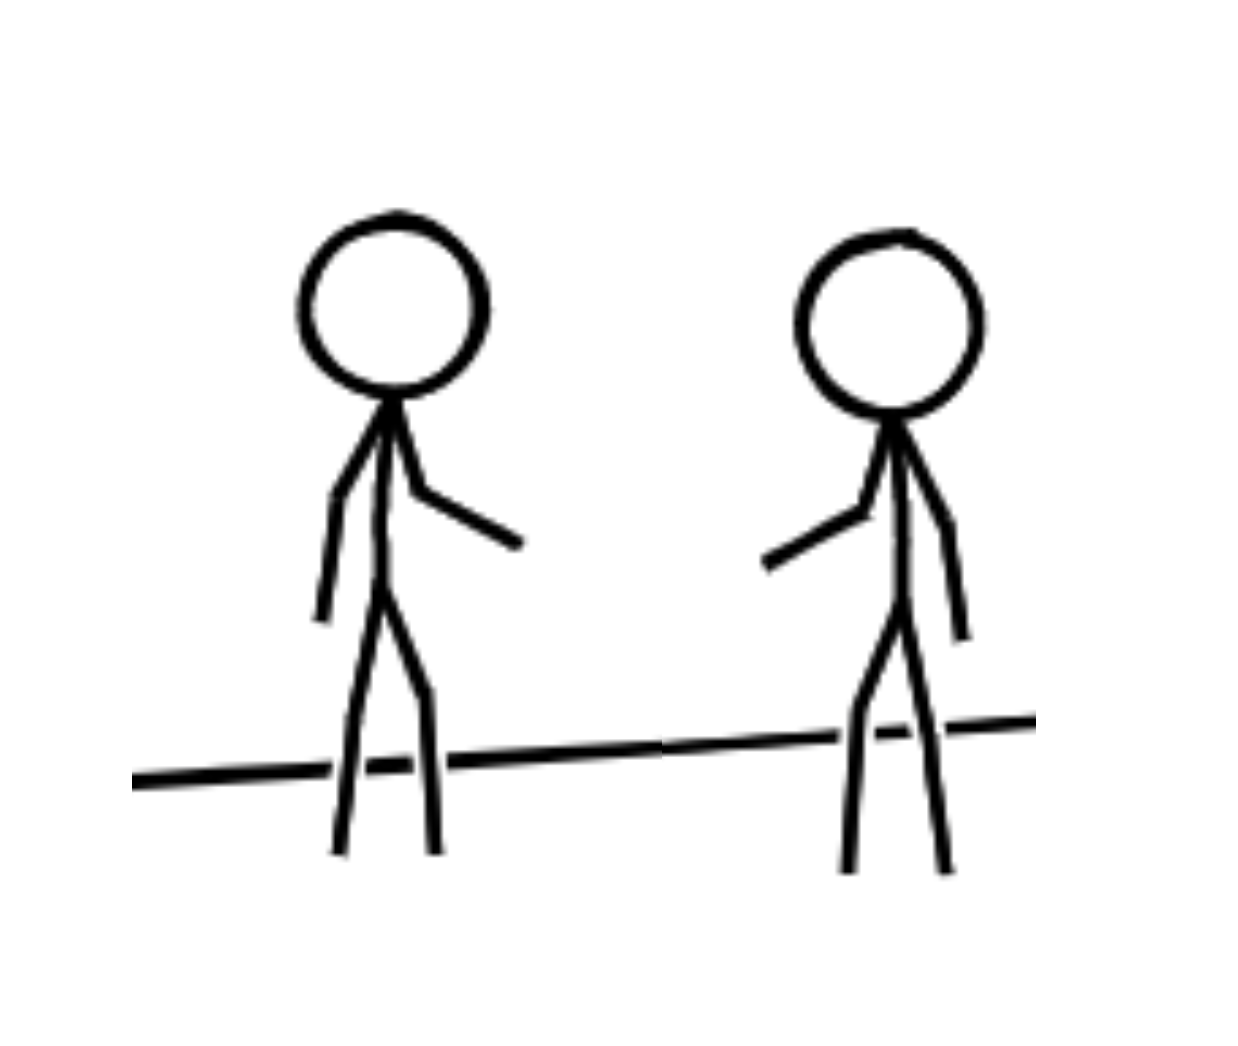
\includegraphics[width=0.19\textwidth]{figures/xkcd_example}
	\vspace{-10pt}
    \caption{An abstract comic example.}
    \label{fig:xkcd}
	\vspace{-10pt}
\end{wrapfigure}

%~\textcite{scott1993understanding} identifies several fundamental components that influence reader reaction: character gestures, inter-character distance, and shading intensity. For example, the gesture of a character can help reader to understand interaction between characters and the emotion of the character. As a common technique, cartoonists often use the gesture to intensify the feeling that they want to communicate to the reader \cite{scott1993understanding}.
% In a persuasive message, the intensified emotion may make the message more memorable than a plain tone.
% We plan to incorporate three variations of each of these elements in our first study.
% As a form of art, the creation of comics has few limitation. Although there is no common template that could describe all comics, if we take a closer look at each comic, it is not hard to see that every comic consists of several fundamental components. We categorize key comic elements into three groups: 1) character gestures, 2) inter-character distance, 3) background shading. To represent a persuasive message in comic form, we need to determine each of those three parameters.
% The gesture of a character is another important component in the comic.

% The relationship between characters is also important. Social proof suggests that messages are more persuasive if the person communicating the ideas is someone the receiver relates \cite{Cialdini1993}.
% In comics, the relationship between characters is modeled by the inter-character distance~\cite{scott1993understanding}.  A rich body of research has demonstrated the relationship between background shading and the emotion in comics~\cite{scott1993understanding}.

% The main research question:

% \textbf{RQ3}: \textit{What the effect of the elements of the comic form, specifically gesture, shading and distance between characters, in modulating comic persuasiveness?}

%!TEX root = cscw2019-comic.tex
\section{Method}
\label{sec:Method}
In this study, we examined if the abstract comic can impact a decision with monetary consequence on Amazon Mechanical Turk. The persuasion task is to ask participants to make a charitable donation decision to the Organization for Autism Research with the real money. 

In this section, we will first discuss the choice of task, then show how we construct persuasive messages (\Cref{sub:Constructing Persuasive Messages}). Then, we introduce our experimental design (\Cref{sub:Experiment Design}), discuss our study procedure (\Cref{sub:Study Procedure}) and participant recruiting process (\Cref{sub:Participant Recruitment}).

\subsection{Choice of Task: Charitable Donation}
\label{sub:Choice of Task: Charitable Donation}
There are many different compelling behavioral contexts on which to test the role of the comic form: personal wellness goals (e.g., diet, exercise), mundane tasks (e.g. ``pick up dry cleaning''), as well as broader public-goods issues (e.g. ``take the flu shot;'' ``donate to cure cancer'').

We identify four criteria that consistent with prior literature \cite{lee2013does, sussman2015framing,saunders2016no,rumsey2003influence} to guide us, in our choice of the experimental behavioral context: nature of the reward; single shot tasks; an ecologically valid task; absence of specialized knowledge to perform the task. First, we would like the rewards to be distant, and non-exclusive, rather than proximal and exclusive so that individuals won't perform the task in anticipation of the immediate reward. Thus public goods dilemmas (e.g. ``reducing carbon footprint;'' ``taking the flu shot''; ``contributing to public knowledge'') are all candidates. Second, while some longitudinal tasks (e.g., losing weight; eating healthy) have distant rewards (losing weight, or maintaining a diet takes time), and can positively affect the public good (with more healthy people, in the long-run, insurance rates will fall), these tasks are prone to habit formation, a potential confound. Furthermore, single-shot tasks such as ``pick up yogurt at the grocery store today'', often prompted by text reminders from our calendars or task-tracking apps, have an immediate, exclusive reward. Third, we would like to ensure that the experimental task is ecologically valid---a task that these individuals would be actually asked to perform in the real world, outside of the experimental context. Fourth, we would like the task not to require specialized knowledge (e.g. ``asking doctors to make a decision''), so that other researchers could easily replicate and scale. 


Online charitable donation tasks satisfy those criteria as 1) they are single-shot tasks, 2) they contribute to the public good with distant, non-exclusive rewards, 3) requests for charitable donations frequently occur online, and 4) the task allows for experimental replication. 


We also considered two other in-the-wild experimental scenarios: buying healthy food and exercise. We considered the task of persuading individuals to buy healthy food by sending them push notifications on the smartphone when they were shopping for groceries. We encountered two challenges. First, we could not control for confounds in the decision making (if there are discounts on salad / healthy items; if the shopper was in a rush; if the shopper was shopping with friends who were pursuing a healthy lifestyle). Second, the reward had a possible confound for some participants, healthier food may make them feel better, and thus they may make the choice to buy healthier food not because of the message, but because of the anticipated reward. We also considered persuading individuals to adopt healthy behaviors, such as taking a walk or going to the gym. Then, we can measure gym visits or exercise outcomes. However, the central challenge here is that those activities are prone to habit formation, a confound. If habit forms, it may be more important in causing repeated behavior than the message received.

In our study, we choose the Organization for Autism Research (OAR) for three reasons. First, Autism Spectrum Disorder (ASD), is a well-recognized developmental disorder that impairs communication and behavior \cite{american2013diagnostic}; ASD provides basic interest for the participants to support the related charitable organization. Second, the Organization for Autism Research is one of the most visible ASD related organizations that helps individuals with autism and provides assistance to their parents, families, teachers, and caregivers. The goal of OAR is clear and reputable so participants won't question the authenticity of our message's motive. Finally, we wished to avoid a charity associated with a life-threatening condition such as cancer as it may create an experimental confound: we don't know if someone donates because their intrinsic desire to help with a life-threatening situation. While ASD can have serious consequences on the well being of those who have it, the public perception is that ASD is not-life threatening \cite{american2013diagnostic}. 


\subsection{Experiment Design}
\label{sub:Experiment Design}
Since the main goal for this study is to compare the power of a persuasive message in two forms, the abstract comics and the text, we first constructed two experimental conditions, the comic condition (see~\Cref{fig:basic three comic panel}) and the text condition. In the comic condition, participants will read a message asking if they are willing to support a charity in a three-panel abstract comic strip, whereas in the text condition, participants will receive the same message in plain text form. 

To test the idea of social proof, we then added a third condition, the comic with the social proof condition. Participants will read a three-panel comic strip that has the same content as the comic condition but added one line text indicating the normative behavior (see~\Cref{fig:basic three comic social proof}). To gather the basic statistics to create social proof, we first ran a pilot study with the first two conditions ($n=60$) on Amazon Mechanical Turk and used the donation statistics as part of the social proof message. In the pilot study, 87\% of the participants donated a non-zero amount. 

\begin{figure}[bt]
    \centering
    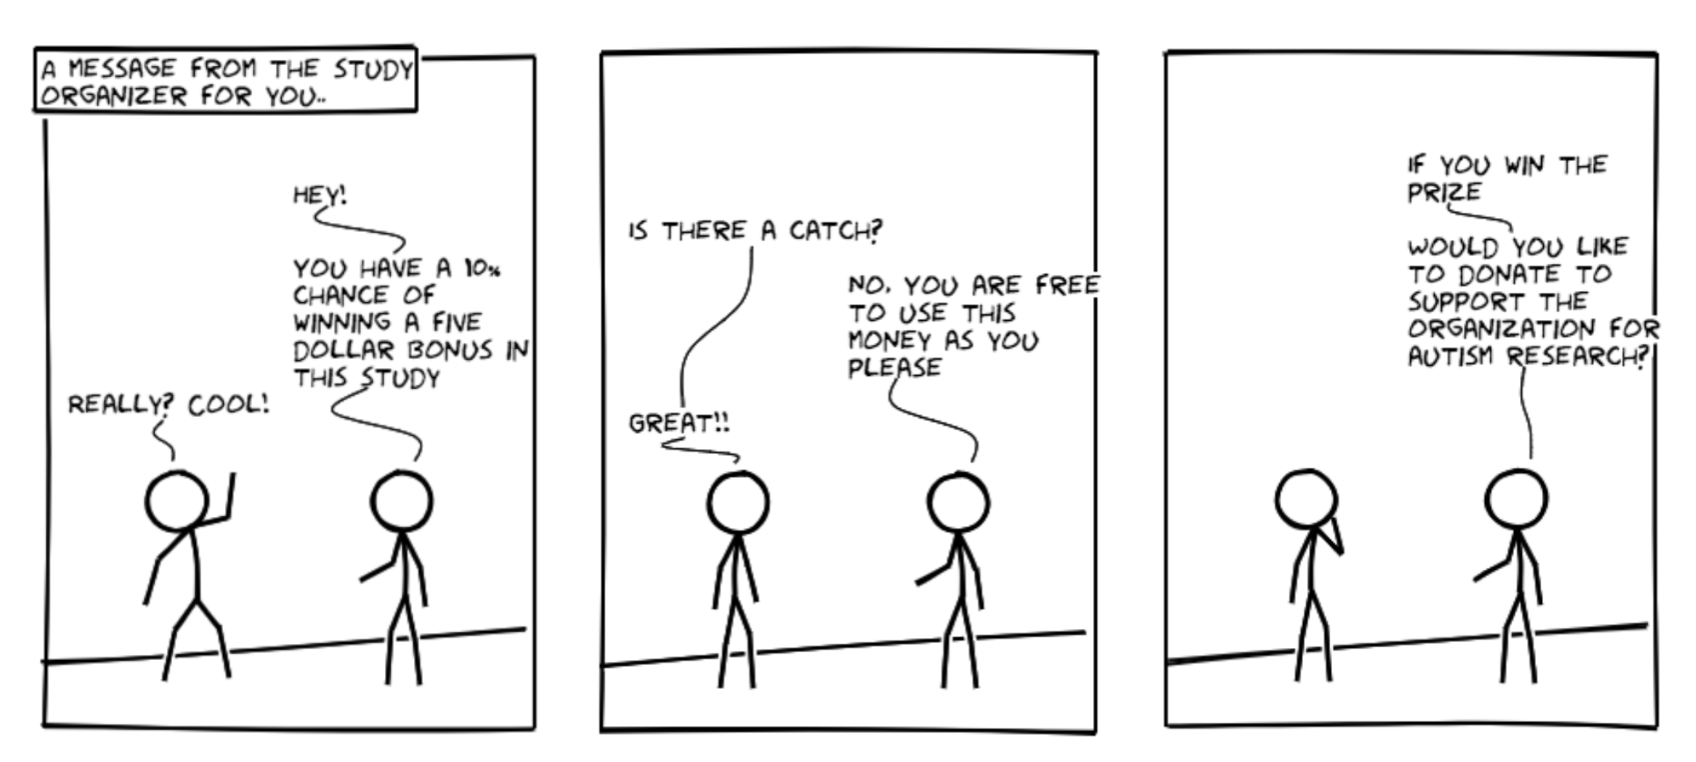
\includegraphics[width=\columnwidth]{./figures/abstract_comic.png}
    \caption{Messages in the abstract comic form. Same as the text messages, the three-panel comic strip communicates three points: 1) Participants will have 10\% of a chance winning \$5 bonus upon the completion of the study (see the first panel); 2) Participants are free to use the money as they please (see the second panel); 3) Participants can donate this bonus to the Organization for Autism Research (OAR) (see the third panel).}
    \label{fig:basic three comic panel}
\end{figure}

The objectives of the persuasive message in all three conditions are the same: persuading participants to donate to a charity from his/her own pocket. Similar to \textcite{lee2013does,saunders2016no}, the money participants will use is part of their study reward, a prospective bonus reward (10\% chance of winning \$5 bonus). We randomly assigned study participants to one of the three conditions; the participants are free to make a decision on the amount of donation, including not donating at all.

\subsection{Constructing Persuasive Messages}
\label{sub:Constructing Persuasive Messages}
Now we discuss construction of the three different messages: a plain text message, a comic, and a comic with social proof. Each message communicates three points: 1) Participants will have 10 \% of a chance winning \$ 5 bonus upon the completion of the study. 2) Participants are free to use the money as they please. and 3) Participants can donate this bonus to the Organization for Autism Research (OAR). Therefore, in the text condition, study participants will read the following message,

\begin{quote}
  \textit{You have a 10\% chance of winning a five dollar bonus in this study. You are free to use this money as you please. If you win the prize, would you like to donate to support the Organization for Autism Research?}
\end{quote}

In the two comic conditions, we created three-panel comic strips to communicate the \textit{same} text message. We used three panels to communicate each of the three points in the message. 

While aesthetic considerations govern the choice of the number of panels in the comic form, two factors influenced our choice of the number of panels: the number of points in the message, and communicating the idea of a conversation, over time, between two individuals. Since we wish to communicate three points (chance of winning bonus; free to use the money as they please; voluntary donation) in the short comic, to ensure that each point was salient, we chose to communicate each point in a different panel. Comic panels along with the text bubbles within a panel fragment time and space. Time flows in two ways: vertically in each panel through the dialogue between the characters and across panels. Since this is a short conversation, three panels seemed appropriate. While adding more panels would elongate the perceived sense of time, we wished to be economical in our communication of the interaction between two characters. We can control of the number of panels in our comic generator (see~\Cref{sec:Discussion}), and we leave the question of how the number of panels (and thus the perceived sense of time) affects message comprehension for future work.

To help the reader connect across panels to achieve closure~\textcite[][Chapter 3]{scott1993understanding} suggests that it is essential to match the panels. Different techniques to match exist, including ``moment-to-moment'', ``action-to-action'', ``scene-to-scene'' etc. help the reader bridge different time scales (see~\parencite[][p. 71]{scott1993understanding} for a summary). We used the ``action-to-action'' matching technique~\cite{scott1993understanding} since all the activity occurs in one scene, and where the activity depicts a brief dialogue between two characters. In particular, we matched the panels on the gesture of the first character (the message recipient), while retaining a neutral gesture for the second character (who delivers the message). 


In the comic with social proof condition, we created social-proof by adding one sentence on the last comic panel indicates the percentage of people in our study donated (\Cref{fig:basic three comic social proof}). The percentage (87\%) corresponds to the number of people who donated a non-zero amount in the pilot study.

For the purposes of this study, we created a comic generator to generate comic strips used in the study. The generator leveraged an open source comic library, ``cmx.io'' ~\cite{cmx.io}, to generate comic figures and used ``rough.js'' \cite{rough.js} to generate other elements such as text bubbles and outline frames. The generator impersonates the style found on ``XKCD''~\cite{munroe2009xkcd} comic. Our focus is not the XKCD style, but the fact that the generated comic is abstract. We believe the generator has the potential to be further developed as a general framework to automatically synthesize pure-textual persuasive messages into abstract comic forms (we discuss this aspect further in section ~\Cref{sec:Discussion}).


\subsection{Study Procedure} 
\label{sub:Study Procedure}
Once participants consented to join the study, we ask them if they are familiar with the Autism Spectrum Disorder (ASD). Then, each participant watched a short video produced by the Organization for Autism Research that promotes its fundraising activity "RUN FOR AUTISM" ~\cite{youtube_research}. After watching the video, we asked participants to summarize the video using free text and ask them to provide their opinion about the effectiveness of the video. The recruiting message specifically mentioned the task is soliciting their opinion on video message's effectiveness. There are two main goals for this part of the study: first, similar to the informational materials (e.g. text) used in other donation studies \cite{lee2013does,10362981,feiler2012mixed}, the video provides context. We want to make sure prior familiarity with autism do not confound our study; second, we want our main task less intrusive as soliciting charitable donation is not a common task on Amazon Mechanical Turk. We did consider establishing context by other means, such as an informative page with text and images on the organization of autism research. We decided against such an approach, because we could not guarantee that all subjects would have read the page. Furthermore, making subjects answer questions about the web-page to check if they had read the page carefully, seemed artificial, impinging on ecological validity. Finally, the linearity of the video is an advantage: subjects could advance to the next page only after watching the video, ensuring consistent knowledge to the best of our ability.

We then randomly assigned participants to one of the three conditions and asked them to read the corresponding persuasive message (text, three-panel comic, three-panel comic with social proof). In the message, we provided the participant with a 10\% chance of winning \$5 additional bonus reward. We also provided them with the opportunity to donate to the Organization for Autism Research (OAR) which is the charity mentioned in the video they previously watched. 

To best demonstrate the persuasiveness of the message, in our messages, we made it clear to participants that they can use the bonus freely as they please. The donation is completely voluntary and irrelevant to the compensation. The default donation amount for everyone is set to \$0 to control for the default effect. Similar to ~\textcite{lee2013does}, we also diffused the responsibility of donation amount among all participants. Before the participants make their decision, they read ``The total amount of money allocated to [the charity] by all the winning participants will be aggregated and donated at the end of the study.'' Then, we asked the participants to decide the amount of money they are willing to donate on a slider bar with \$0 and \$5 as two extreme ends. To increase the realism of our study, the donation decision is not hypothetical: the winning participants receive the amounts that they choose keep; as study organizers we donate to the Organization for Autism Research (OAR) the cumulative sum of the participant donations. 

Before leaving the study, participants need to filled a demographic questionnaire about their gender, income and education; participants had the option of declining to state an answer for each question.

At the end of the study, we randomly chose 10\% of the participants, donated to OAR based on their decision, and rewarded them with part of the bonus that they wished to keep.

\begin{figure}[bt]
    \centering
    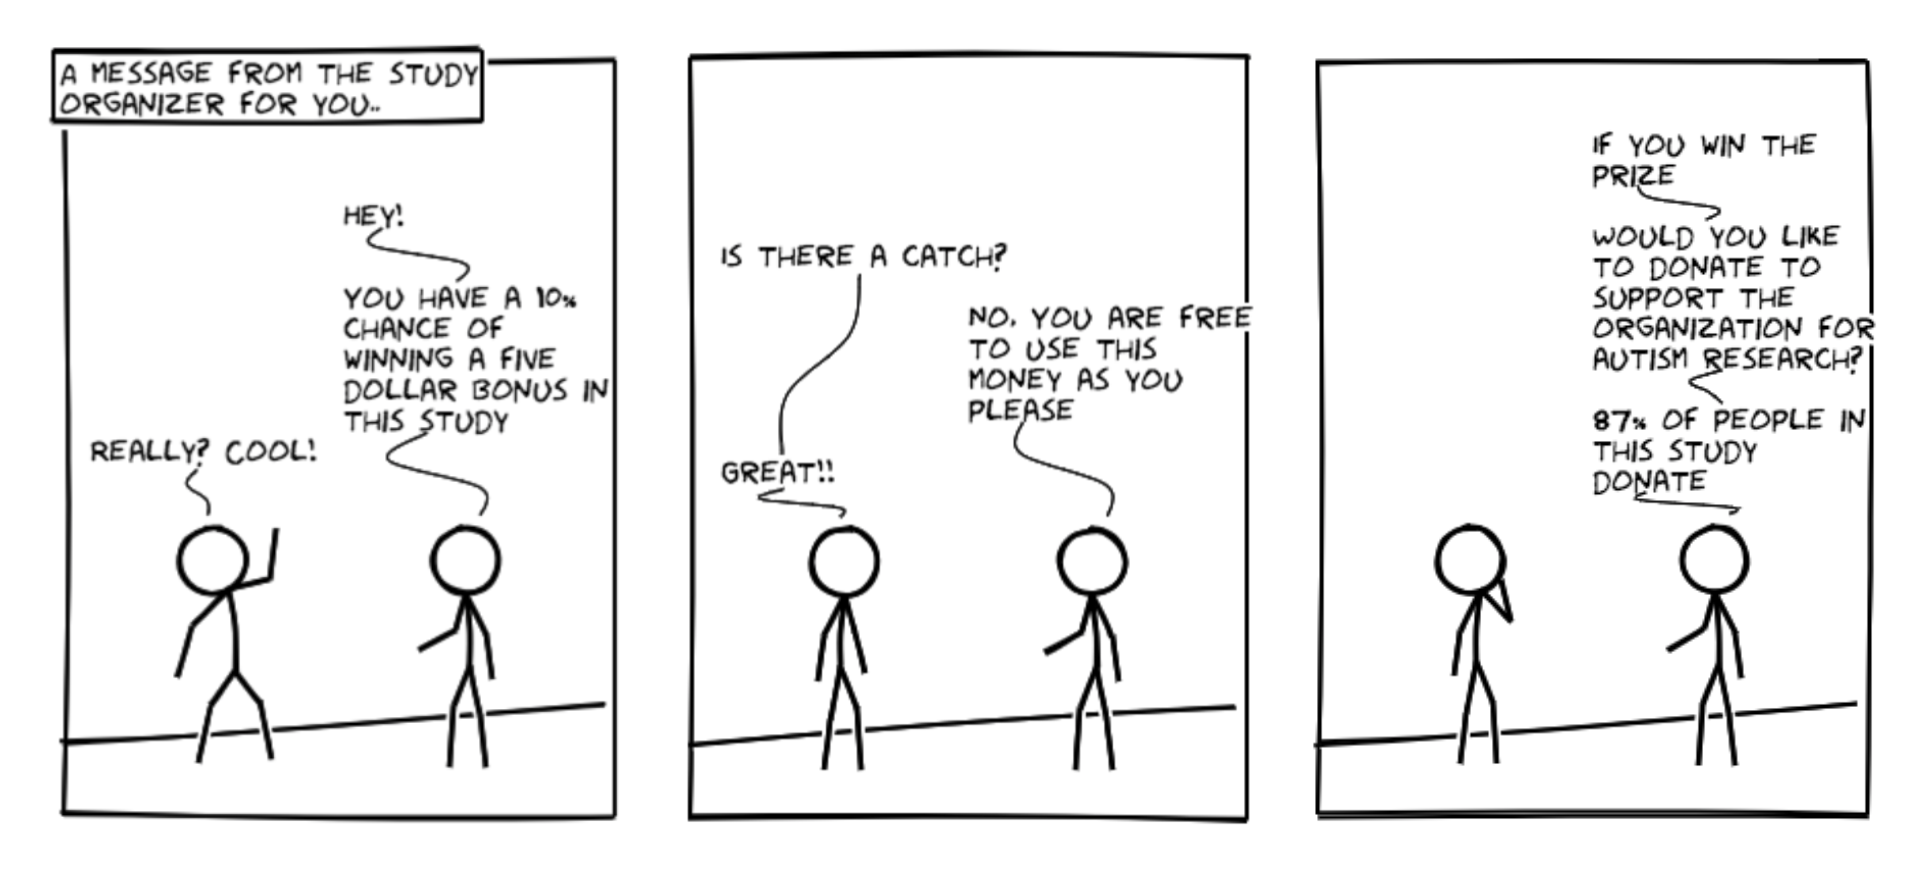
\includegraphics[width=\columnwidth]{./figures/social_proof.png}
    \caption{Messages with social proof. In addition to the three points that we wish to communicate (chance of winning bonus; free to use the money as they please; voluntary donation), the comic with social proof communicates the idea of the social proof at the third comic panel. The figure ``87\%'' comes from our pilot study}
    \label{fig:basic three comic social proof}
\end{figure}



\subsection{Participant Recruitment}
\label{sub:Participant Recruitment}
In this study, we recruited our study participants from Amazon Mechanical Turk. Although the Amazon Mechanical Turk, a crowdsourcing platform, has been widely used to gather human intelligence in AI research and social science experiments \cite{ paolacci2014inside,berinsky2012evaluating,buhrmester2011amazon,branas2018gender,lee2013does,saunders2016no,arechar2017turking,sussman2015framing}, we should be cautious when using such platform as the participant selection criteria is not transparent \cite{landers2015inconvenient,paolacci2010running}. In our study, we chose the Amazon Mechanical Turk for the following reasons. First, our persuasion task is about online charitable donation which targets internet users. Second, crowdsourcing platforms will help us reach a more diverse sample than using the researchers' own social network to attract participants \cite{buhrmester2011amazon}. Third, the main motive for Amazon Mechanical Turk workers is monetary rewards \cite{berinsky2012evaluating}. In our study design, Amazon Mechanical Turk subjects may be more sensitive to the monetary reward they receive, making them less amenable to persuasion. Finally, the use of Amazon Mechanical Turk subject pool by multiple studies~\cite{branas2018gender,lee2013does,saunders2016no,arechar2017turking,sussman2015framing} on charitable donation decisions informed our decision to use the Amazon Mechanical Turk subject pool. 

Motivated by studies that show that populations on Amazon Mechanical Turk are diverse and mirror the US population \cite{buhrmester2011amazon,behrend2011viability,berinsky2012evaluating}, we recruited our participants from Amazon Mechanical Turk. However, we are aware of research that raises concerns in Amazon Mechanical Turk's sample representativeness \cite{landers2015inconvenient,paolacci2010running}. One potential solution is to use a panel company's population (e.g., Qualtrics). However, this method also has concerns in that the researcher can not directly cross-validate the sample's representativeness---we have to trust the company's assertion.

We published our HITs on Amazon Mechanical Turk titled ``A short survey about communicating autism campaign ads``. The compensation was \$10/hr, and the workers would get the compensation regardless of their performance. To ensure quality, the HIT is limited to English Speakers in US and people who have a 95\% Approval Rate. On the HIT page, we instructed that repeated responses would be rejected. We told the participants that they would see a link to our experiment site (Qualtrics). 

%!TEX root = cscw2019-comic.tex
\section{Results}
\label{sec:Study on Behavior Results}

In this section, we will first present the raw data used in the analysis, then introduce the Bayesian Model we used for data analysis and our analysis result.

\subsection{Raw Data}
\label{sub:Study on Behavior Raw Data}
In total, we have 307 participants joined our study, 101 participants received the message in the text form, 102 participants received the same message in the abstract comic form, and 104 participants received the abstract comic message with social-proof. We ran an outlier analysis using Tukey Fence on participants' completion time and removed 30 participants from our dataset. The following analysis is based on a dataset with 277 participants, 91 of them is in pure-text condition, 97 of them is in comic condition, and 92 of them is in comic-social-proof condition. Of those 277 participants, 150 were self-identified as male, and 126 were self-identified as female, 1 participant chose not to disclose. 197 participants earned at least college degree. The median annual household income of our study participants is \$50,000 - \$59,999, which is close to the median annual household income in US (\$ 57,652).\footnote{From 2017 US Census Data https://www.census.gov/quickfacts/fact/table/US} 72 \% of study participants earned at least college degree. All participants were familiar with the Autism Spectrum Disorder and acknowledged the importance of autism research. 

~\Cref{fig:contributions across conditions} compares the distributions of the charitable donations across the three conditions. Among all 307 participants, 253 (82.4\%) participants donated non-zero amount to support the autism research; 74 (73.3\%) participants from the text condition, 86 (84.3\%) participants from the comic condition, and 93 (89.4\%) participants from the comic with social proof condition.


\begin{figure*}[htb]
	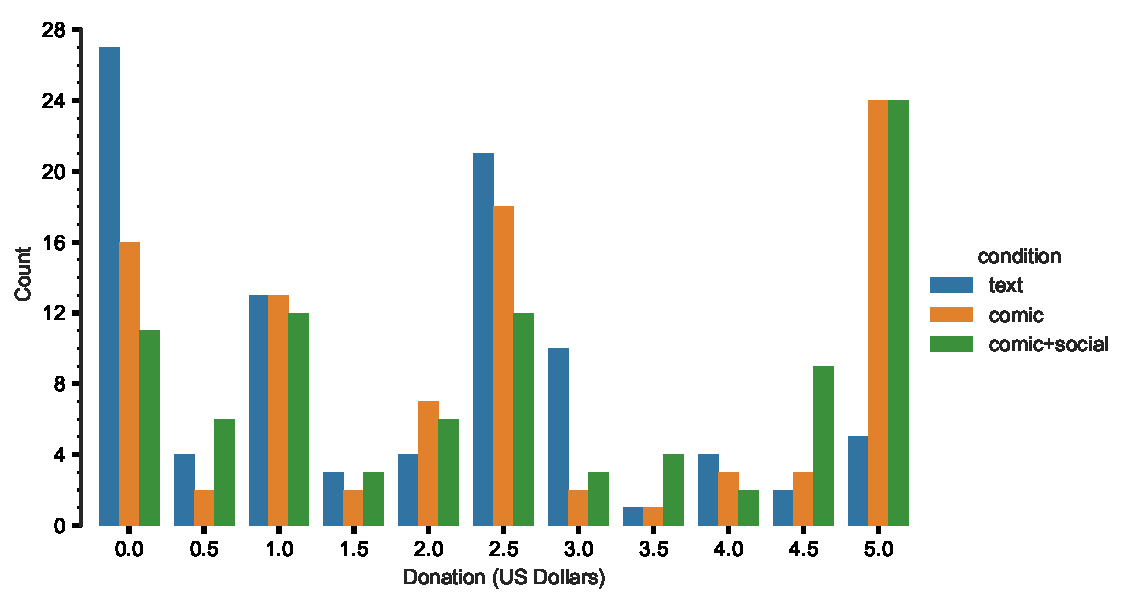
\includegraphics[width=1\textwidth]{./figures/contributions_across_conditions.pdf}
    \caption{The distribution of the amount of money participants decide to donate to the charity in each of the three conditions: text only; comic; comic with social proof. Among all 307 participants, 253 (82.4\%) participants donated non-zero amount to support the autism research; 74 (73.3\%) participants from the text condition, 86 (84.3\%) participants from the comic condition, and 93 (89.4\%) participants from the comic with social proof condition.
}
	\label{fig:contributions across conditions}
\end{figure*}

\subsection{Bayesian Formulation}
\label{sub:Bayesian Formulation}
We use a Bayesian formulation of the problem of identifying suitable predictors for the messages in comic form.~\textcite{Kay2016} provide a nice introduction on the appropriateness of Bayesian analysis for the HCI community. Bayesian analysis is attractive in our experiment due to two advantages: shifting the conversation from ``did it work'' to ``how strong is the effect''; and benefits to small $n$ studies. 

Our experiment has three experimental groups: text, comic and comic with the social proof. One way to use classical statistical analysis for multiple groups would be to use ANOVA to see if the treatment (the use of comic) has any effect.  Bayesian inference can sometimes differ from the standard ANOVA test widely used to compare treatment effects.


This is because ANOVA assumes equal variances within groups, and that the response within each group is drawn from a Normal distribution---in practice, both assumptions may be violated.  It is straightforward in Bayesian Analysis to relax both assumptions: equal variances and Normality. The Normality assumption may be one reason why ANOVA and the $t$-test may be less sensitive to differences than Bayesian analysis~\parencite[][p. 470]{Kruschke2014}.

\begin{figure*}[htb]
    \centering
	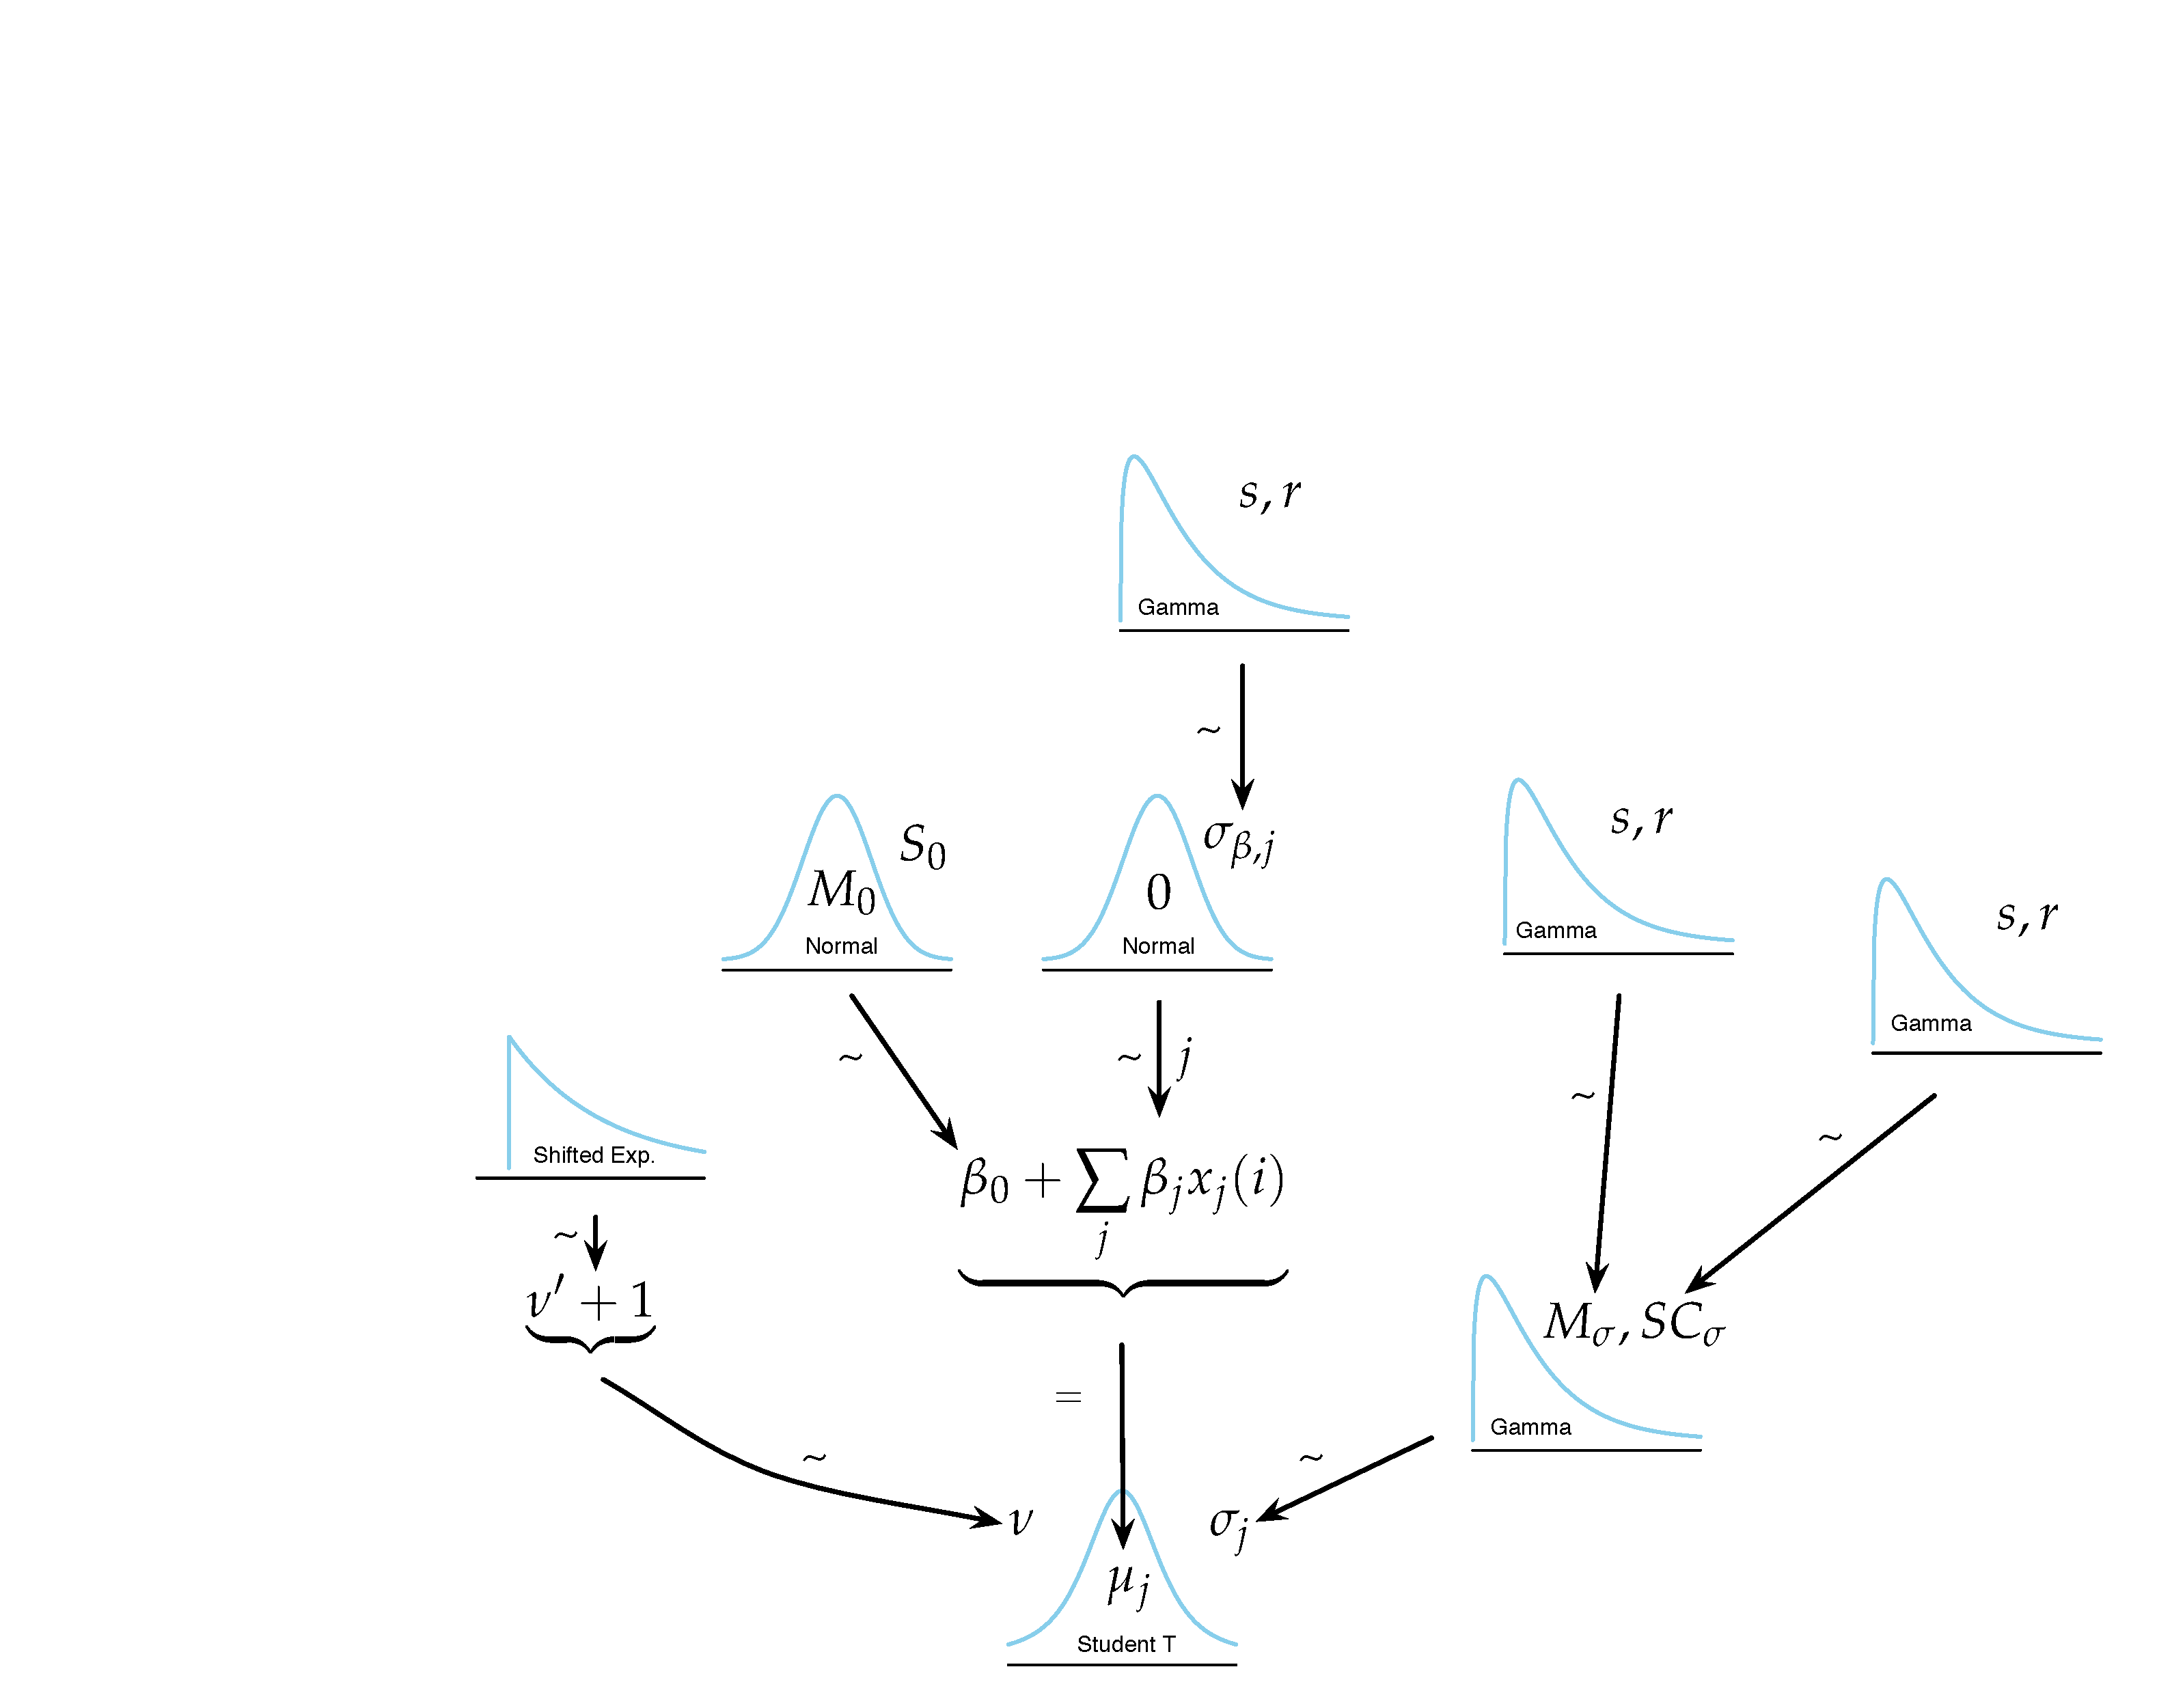
\includegraphics[trim = 4in 0in 0in 4in, clip=true, width=1\textwidth]{./figures/gen_model.pdf}
    \caption{Our proposed Hierarchical Bayesian model. The bottom of the figure shows the Student-t likelihood function for each experimental condition $j$. The likelihood function has three parameters: $\nu$ (degrees of freedom), $\mu_j$ (the mean for condition $j$), $\sigma_j$ (the scale for condition $j$). The prior distribution for $\nu$ is a shifted experimental distribution, so that $\nu\geq 1$. The prior distribution for the class mean $\mu_j$ is a sum of Normal variables, where $\beta_0$ is the central value across all three conditions, and $\beta_j$ is the deflection corresponding to experimental condition $j$. Notice that $x_j(i) = 1 \iff$ participant $i$ is in condition $j$. We draw the variance of $\beta_j$ from a  Gamma distribution to ensure that $\sigma_{\beta, j} > 0$. We draw the scale parameters $\sigma_j$ from the same Gamma distribution. We draw the mode ($M_\sigma$) and the scale ($S_\sigma$) parameters from a Gamma distribution to ensure $M_\sigma>0$, and $S_\sigma > 0$. We set constants $M_0, S_0, s, r$ to result in uninformative (i.e. conservative) priors.
    }
	\label{fig:generative model}
\end{figure*}



Now, we discuss our Bayesian formulation (see~\Cref{fig:generative model} for a graphical view of the model). There is one outcome variable $y_{i \mid j}$, the amount of donation to the charity by each participant $i$, under experimental condition $j$: text, comic, and comic with social proof. 

In a Bayesian model formulation, we first need to define a likelihood function, to describe the data. We adopt the view advanced by~\textcite{McElreath2015} that a model represents an \textit{epistemological} claim (how the modeler views the data), not an \textit{ontological} claim (i.e. a physical assumption about the world). Typically, the likelihood function is parametric, and we may treat each parameter as a random variable drawn from a distribution with parameters (this is the prior of the model parameter); thus Bayesian models can be hierarchical. In Bayesian modeling, the goal is to be conservative, and we express priors that are weakly informative---a technical term that informally means that the prior allows all possible values for the parameter, but does so in a way that allows for rapid model convergence.

We use a Student-t distribution to characterize the donations, since~\Cref{fig:contributions across conditions} shows significant contributions for amount \$0 and \$5. A Student-t distribution is heavy-tailed, in the sense that the Student-t distribution doesn't fall off as quickly as does a Normal distribution. If we choose a Normal distribution to model contributions in each condition, then we would find it harder to explain contributions at \$0 and at \$5, without increasing the Normal distribution variance parameter. The Student-t distribution has three parameters: the degrees of freedom ($\nu$), the experimental condition dependent mean ($\mu_j$) and scale ($\sigma_j$). Since our goal is to understand the average tendency to give to charity under the different conditions, and not to make predictions (as might be the case if we were trying to model donation with age as a predictor), the fact that the $t$-distribution is not bounded is less relevant here.  Each of these parameters are random variables, and we need to define likelihood functions of each of them. Our Bayesian model (also see~\Cref{fig:generative model} ):


\begin{align}
    y_{i \mid j} \sim &  \mathrm{Student-t}(\nu, \mu_j, \sigma_j),  & \text{likelihood function to model donation}\label{eq:bayesian formulation}\\
    \nu \sim & 1 + \exp(\lambda), & \text{degrees of freedom}\\
    \mu_j \sim & \beta_0 + \sum_j \beta_j x_j(i), & \text{modal contribution in each condition } j\label{eq:mean response}\\
    \sigma_j \sim & \Gamma(M_{\sigma}, SC_{\sigma}), & \text{scale parameter for condition } j\\
    M_{\sigma} \sim & \Gamma(s,r), & \\
    SC_{\sigma} \sim & \Gamma(s,r), &  \\
    \beta_0 \sim & N(M_0, SD_0), & \text{average contribution across conditions}\\
    \beta_j \sim & N (0, \sigma_{\beta, j}), & \text{deflection from average contribution for condition } j\\
    \sigma_{\beta, j} \sim & \Gamma(s,r) & .
\end{align}
 
\Cref{eq:bayesian formulation} says that the response $y_{i \mid j}$ of each group $j$ is modeled as a $\mathrm{Student-t}$ distribution with mode $\mu_j$,  scale $\sigma_j$ and with $\nu$ degrees of freedom; notice that this is a \textit{drawing distribution}, not the $t$-test. The Student-t allows us to model a non-Normal outcome with a heavy tail; assuming $y_{i \mid j}$ to be Normally distributed is equivalent to setting $\nu=\infty$. Now we explain the the main parameters of the model.


\begin{description}
    \item[Degrees of Freedom:] We draw the degrees of freedom $\nu$ from a shifted exponential distribution, to ensure $\nu \geq 1$
    \item[Modal contribution $\mu_j$ in each condition $j$:] The mode $\mu_j$ corresponding to each group is drawn from a sum of Normally distributed random variables with $\mu_j = \beta_0 + \sum_j \beta_j x_j(i)$, where $\beta_0$ corresponds to the overall mean contribution across experimental conditions, and where the group indicator variable $x_j(i)=1 \iff \text{subject } i \text{ belongs to group } j$. We model the overall group response $\beta_0$ as a Normal distribution with mean $\mu_0$ and variance $\sigma_0$. For each of the $\beta_j$ for each group $j$ in~\Cref{eq:mean response}, $\beta_j$ is Normally distributed with mean $\mu=0$ and $\sigma_{\beta, j}$ drawn from a Gamma distribution $\Gamma(s,r)$ with shape parameter $s$ and rate parameter $r$, ensuring $\sigma_{\beta, j} > 0$. 
    % We set the variables $s,r$ to allows a wide range of values for $\sigma_{\beta, j}$.  
    The random variables $\beta_j$ are centered around $\mu=0$ so that the group responses are modeled as deflections around the overall mean $\beta_0$. Notice that we draw the variances $\sigma_{\beta, j}$ of each group $j$ independently from a Gamma distribution with same parameters ($s,r$), implying that the variances (equivalently, the extent of deflections from the mean) for each predictor $\beta_j$ can be different. The main advantage of using a Gamma distribution is that we can specify a non-zero mode, important in controlling shrinkage in hierarchical models. 
    \item[Scale $\sigma_j$ of each condition $j$:]  The scale $\sigma_j$ of the likelihood function is drawn from a Gamma distribution $\Gamma(M_{\sigma}, SC_{\sigma})$, with mode $M_{\sigma}$ and scale $SC_{\sigma}$; this prior on $\sigma_j$ ensures that $\sigma_j > 0$. The mode $M_{\sigma}$ and scale $SC_{\sigma}$ are each drawn from two independent Gamma distributions $\Gamma(s,r)$ with shape parameter $s$ and rate parameter $r$. The advantage of this hierarchical approach is that the values of each element of $\sigma_j$ inform the other elements. The ``information sharing'' among variables common to hierarchical Bayesian models and is an important reason why Bayesian models work so well with small datasets\footnote{The sharing of information causes the scale of each group $\sigma_{j}$ to move towards the group variance, a phenomenon known as ``shrinkage.'' }.
    \item[Constants:] The constants $M_0, S_0, s, r$ are set so that the priors are generous but weakly informative so that despite exploring all possible values, we ensure rapid MCMC convergence.
\end{description}


Having introduced our model, now we examine the results of the data analysis.


\subsection{Analysis}
\label{sub:Analysis}

We analyzed the data using PyMC3~\cite{Salvatier2016}, a popular framework for Bayesian inference. Computational techniques for Bayesian inference use a stochastic sampling technique called Markov Chain Monte Carlo (MCMC) that samples the posterior distribution $P(\theta | D)$, where we want to estimate the parameters $\theta$ given the observations $D$. In particular, we used the No-U Turn Sampler (NUTS) sampler. 

\begin{sidewaysfigure*}
    \centering
	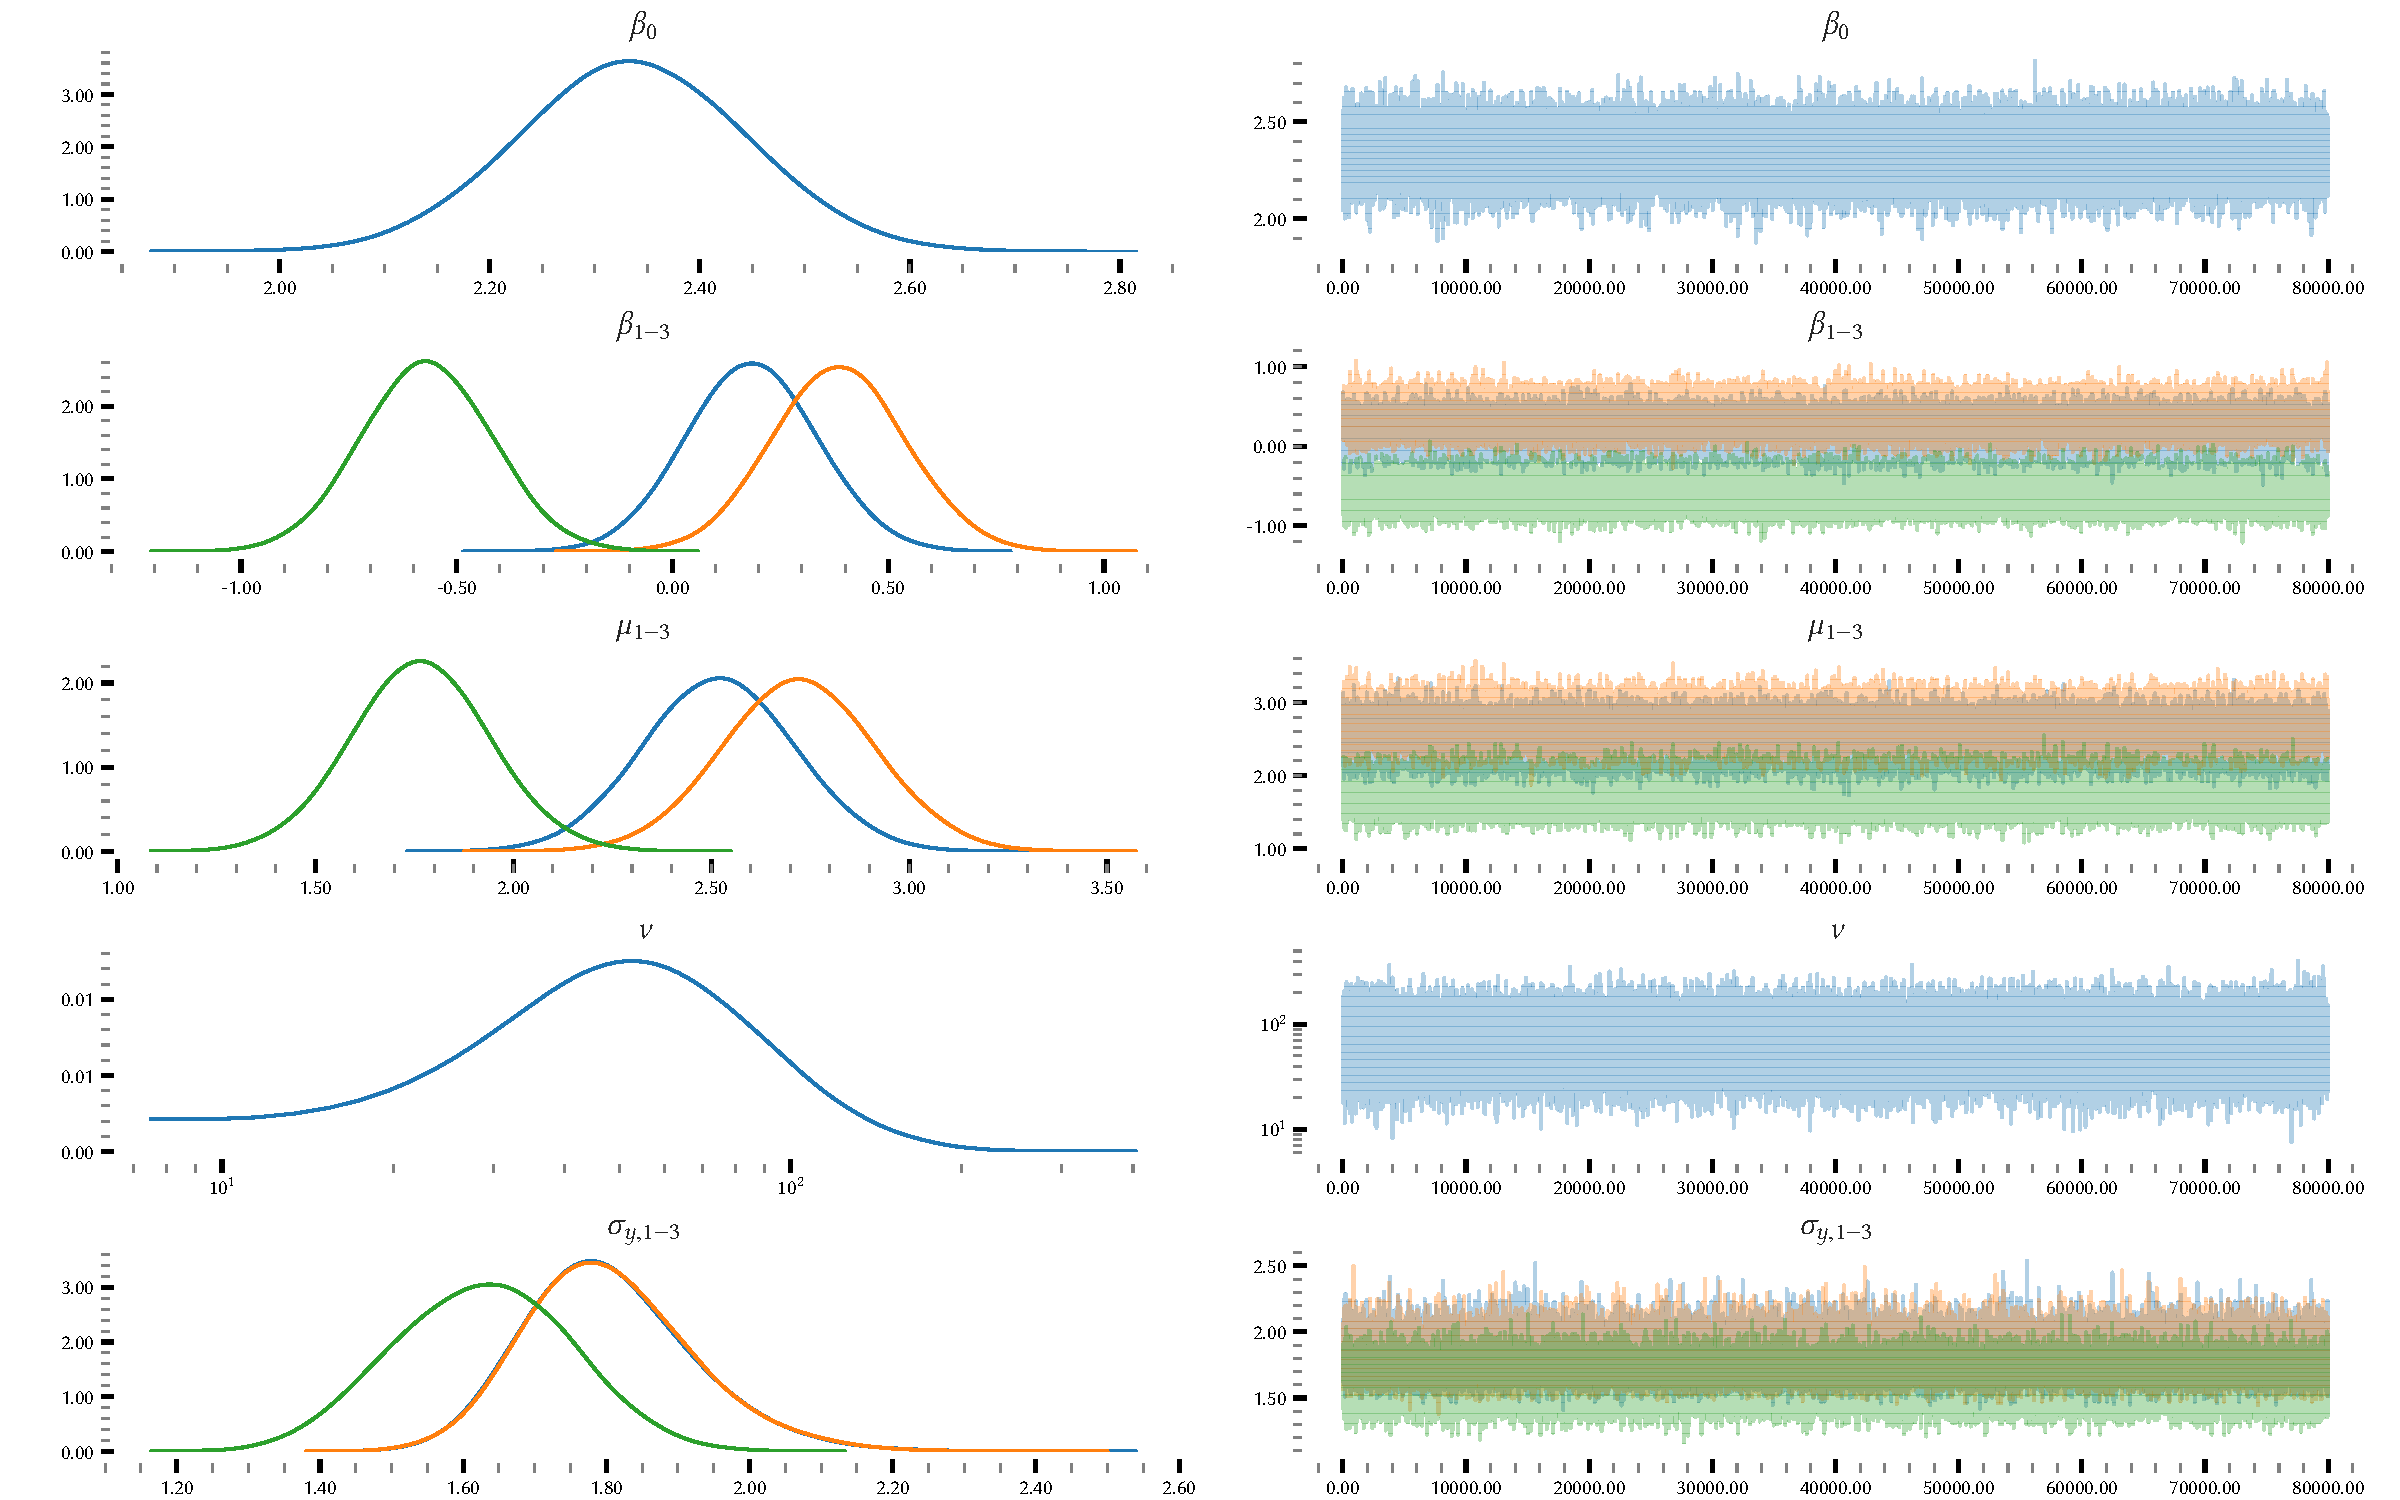
\includegraphics[width=0.8\textwidth]{./figures/robust_traceplot.pdf}
    \caption{Traceplot showing the results of the MCMC estimation. Left column shows the posterior distributions for $\beta_0, \beta_{[1-3]}, \mu_{[1-3]}, \nu, \sigma_{[1-3]}$, while the right column shows the corresponding traces. The posterior plots for $\nu$, the parameter corresponding to degrees of freedom has a modal value of $\nu=53$. While the ideal case of $\nu=\infty$ makes the Student-t distribution equivalent to the Normal distribution, in practice $\nu \geq 30$ is used to test for Normality. Thus the response distributions $y_{i \mid j}$ tend towards Normality. Notice that the mean of $\sigma_2$ (green curve, fourth panel, left column), variance of the group response in the case of text, is less than $\sigma_1$ or $\sigma_3$ (variances of the group responses for the comic, comic+social norm cases respectively), justifying our modeling assumptions of unequal variances across groups; the variances for the two comic conditions are nearly identical. The Gelman-Rubin statistic $\hat{R}$ was around 1, indicating that the different sampling chains converged. Furthermore, the effective sample size of all parameters was greater than 10,000. }
	\label{fig:traceplot}
\end{sidewaysfigure*}

 

Our analysis shows that the abstract comic form has a clear treatment effect over the corresponding text message.~\Cref{fig:robustcontrasts} shows the contrast and the effect size of the contract for four cases. The first three columns of~\Cref{fig:robustcontrasts} show the contrasts (top row) and the corresponding effect size (bottom row) between a pair of experimental conditions. The fourth column is a comparison between the text condition and the comic condition, by pooling together responses of the two comic conditions.

Let us examine one result (`text' v. `comic') in detail; the analysis for the other cases follows a similar logic. The top left sub-figure shows that the contrast has a mode of $0.75$ with the High Posterior Density (HPD\footnote{The HPD interval is the location of 95\% of the posterior density. This is similar to, but different from the idea of the confidence interval used in non-Bayesian Statistics. In non-Bayesian Statistics, a confidence interval of say 95\% is informally interpreted as ``with 95\% probability the parameter of interest lies in a specific interval; the tails are of equal width (i.e. 2.5\%)''; the HPD on the other hand, is the \textit{densest} interval covering 95\% of the posterior. The HPD is guaranteed to include the most likely value, but this is not always true for confidence intervals; see~\textcite[][p. 57]{McElreath2015} for a simple example. For a more careful definition of the confidence interval, see~\textcite{Hoekstra2014}, which also includes a discussion on the misinterpretation of confidence intervals.}) interval of $[0.26, 1.27]$. That is, subjects most frequently donate $\$0.75$ more on in the comic condition than in the text condition, with 95\% of the \textit{increase in donations} lying between $[\$0.26, \$1.27]$. Since the HPD lies outside a significant ROPE (Region of Practical Equivalence)\footnote{Unlike non-Bayesian Statistics, where one can ask for example, if the two means for two treatments are different $P(\mu_1\neq \mu_2)$, in Bayesian statistics, one asks if the HPD interval of the distribution $P(\mu_1-\mu_2)$, that is, the distribution of the difference of the means of the two treatments, excludes an interval where we can consider the two treatments equivalent. This equivalence interval is domain dependent. } of $0 \pm 0.1$, the result implies that there is a clear effect due to the treatment. Furthermore, the lower left sub-figure shows a moderate to medium effect size of $0.44$; we consider an effect of $0.2$ to be small, and an effect of $0.5$ is a medium-sized effect. Since the distribution excludes the ROPE interval $[0 \pm 0.1]$, half of the small-sized effect value of $0.2$, the discovered effect size is statistically significant. 

The second column contrasts the comic with social proof case (`comic+social') with the plain text (`text'). We find that the contrast has a mode of $0.95$ with the High Posterior Density (HPD) interval of $[0.44, 1.47]$. The modal effect size is $0.55$, with an HPD interval of $[0.25, 0.86]$ which excludes a ROPE of $0 \pm 0.1$ indicating a significant, slightly larger than a medium-sized effect.

The third column contrasts the donations in the comic (`comic') condition against the comic with the social proof (`comic+social'). While the contrast is positive with a mode of $0.19$, notice that the HPD interval $[-0.31, 0.72]$ overlaps a ROPE of $0 \pm 0.1$ implying that the observed differences are not significant. The corresponding modal effect size of this contrast is $0.11$ with an HPD of $[-0.17, 0.39]$ with about 21.9\% of the HPD lying to the left of 0, implying that the observed effect size is not significant.


\begin{figure*}[htb]
	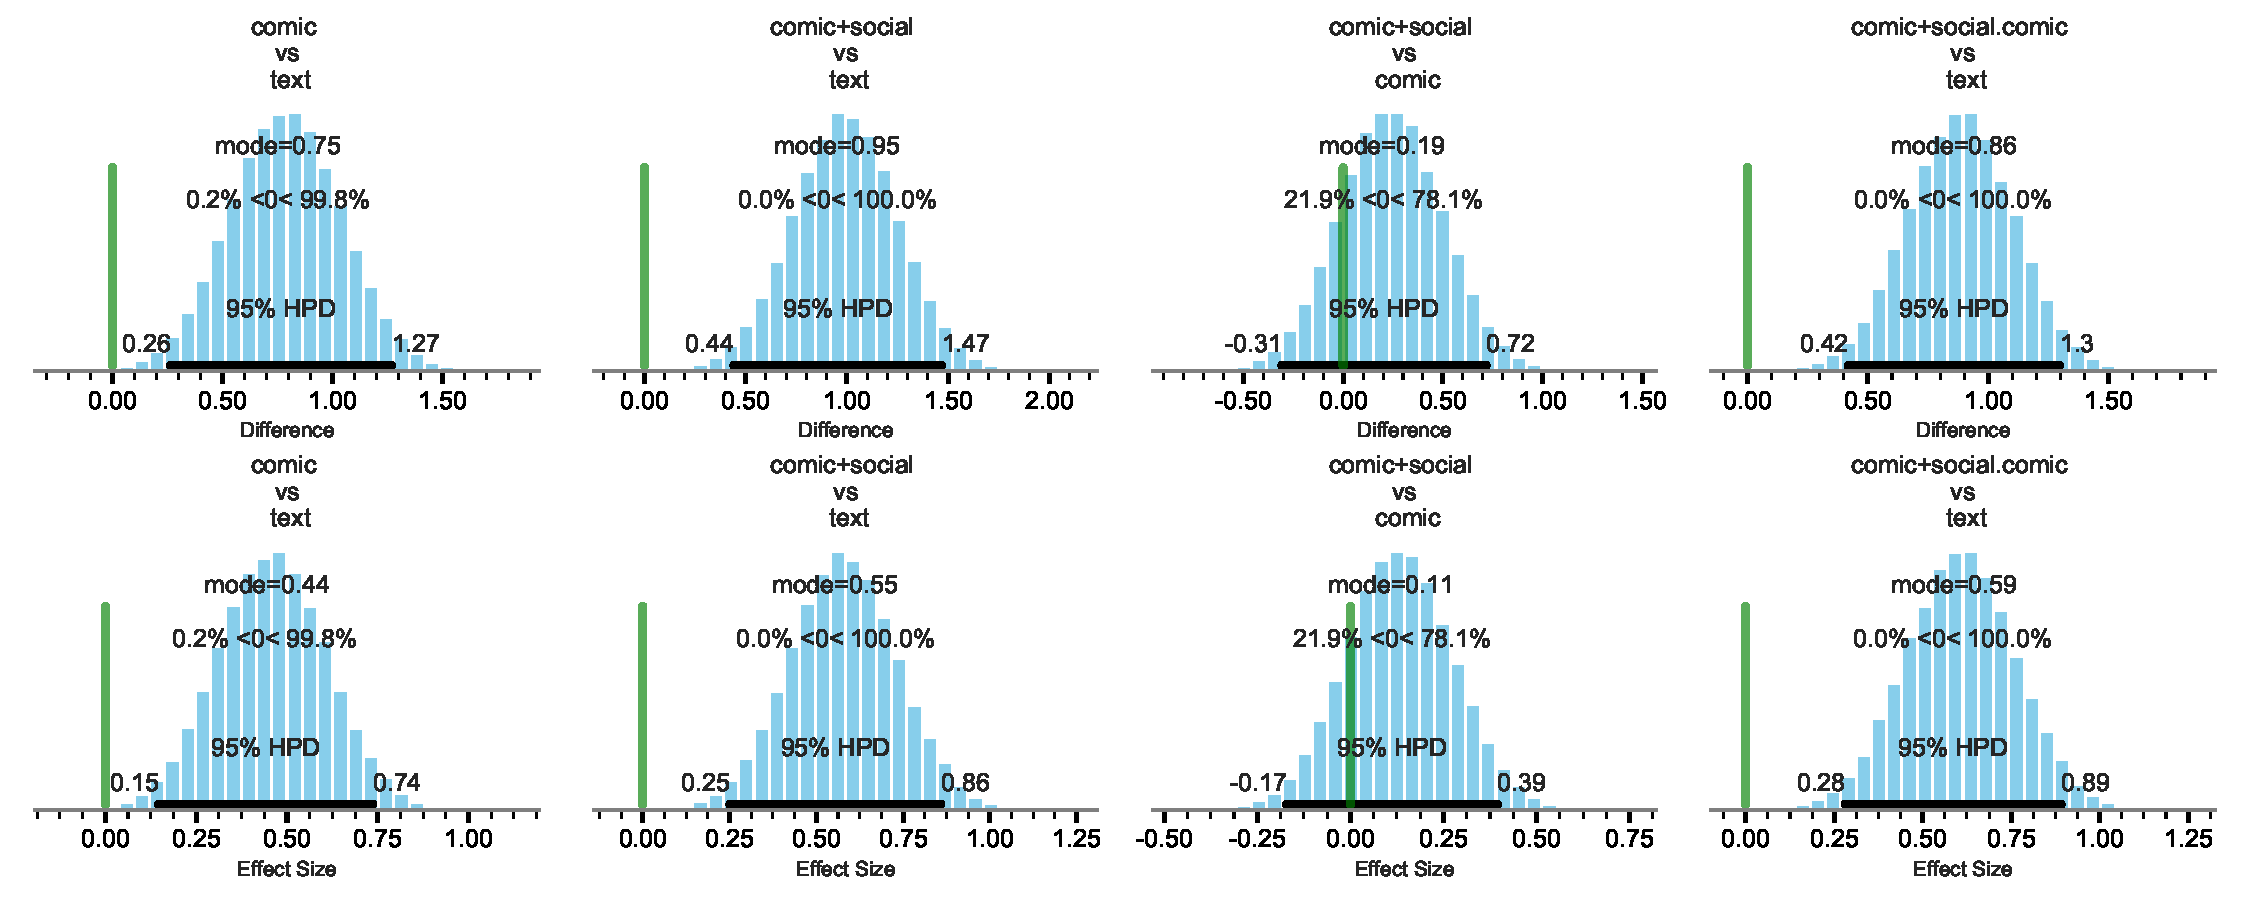
\includegraphics[width=1\textwidth]{./figures/robust_contrasts.pdf}
    \caption{The figure shows contrasts between the three experimental conditions (`text', `comic', `comic+social'). We also show in the fourth column contrasts between the text condition and pooled case of the two comic conditions to highlight the effect of using the abstract comic. Since we are highlighting contrasts, each sub-figure also shows a green line located at 0.The main finding: the comic treatment creates a medium to large sized effect (mode=0.59, pooled case, fourth column, bottom) when compared to the `text' condition. There is a slight increase in effect size when using the comic with social proof (`comic+social', second column, bottom) in comparison to the case when there is a comic without the social proof (`comic', first column, bottom). However, these differences are not significant, since the about 21.2\% of the HPD of the contrast between the `comic' and the `comic+social' case lies to the left of 0.0 (second column). }
	\label{fig:robustcontrasts}
\end{figure*}

The fourth column of~\Cref{fig:robustcontrasts} compares the text condition (`text') with the comic condition by pooling the responses in the two comic conditions. The pooling of the `comic' and the `comic+social' data is straightforward in Bayesian analysis. Since the MCMC \textit{jointly} estimates the posteriors of all variables, we can create a new variable that averages the values of the posteriors of the `comic' and `comic+social' cases for every step of the MCMC, to represent an averaged 'comic' condition.  We find that the contrast has a mode of $0.86$ with the High Posterior Density (HPD) interval of $[0.42, 1.30]$. Notice that the HPD interval is narrower than the corresponding HPD intervals comparing (`text' v. `comic' ) and (`text' v. `comic+social') The modal effect size is $0.59$, with an HPD interval of $[0.28, 0.89]$ which excludes a ROPE of $0 \pm 0.1$ indicating a significant, a medium to large sized effect, where the large effect size is $0.8$. 

In this section, we presented a Bayesian model to analyze the overall effect of using an abstract-comic to persuade people making charitable donation decisions, and understand the effect of adopting persuasive techniques in the abstract comic form. The results show that the use of abstract-comic produces a significant, medium to large modal effect ($0.59$) in persuading participants to donate. Although abstract-comic with social proof (`comic+social') can produce a larger effect that the case without social proof (`comic'), the contrast between abstract-comic and abstract-comic with social proof is not significant. The code and data are available online \footnote{\url{http://ziangxiao.github.io/Abstract_Comic_Persuasion/}}. Next, we discuss the findings, design implications and limitations.

%!TEX root = cscw2019-comic.tex
\section{Model Criticism}
% \section{Model Criticism}
\label{sec:Model Criticism}

In this section, we  begin with a short section explaining our choice to use Bayesian analysis. Then in~\ref{sub:Posterior Checks, Convergence and Normality}, we examine model convergence and Normality.

% how well the proposed models explain the observed data, including model convergence.

\subsection{Why Bayesian?}
\label{sub:Why Bayesian?}
In a recent paper,~\textcite{Kay2016}, make a persuasive argument that Bayesian methods are better suited to the HCI community, including making the case that Bayesian methods allow for replicating the results and improving the strength of the conclusions by using previous outcomes as priors. We would add two reasons, in addition to those by~\textcite{Kay2016} to explain our decision to use Bayesian models. 
\begin{description}
    \item[Transparency:] With a Bayesian model, the researcher foregrounds all the aspects of the model; there are no modeling assumptions that need checking, not already foregrounded in the model description. Non-Bayesian statistics are powerful tools, and when used by an experienced statistician, they can dramatically reduce the process of inference. However, for researchers who wish to investigate their findings without access to a statistician, they need to be careful of the assumptions of the different tests: Normality ($t$-test); heteroscedasticity (e.g., ANOVA) and ensuring that the data satisfy the assumptions. Omitting the right sequence of analysis can lead to inferences not supported by the data.
    \item[Small $n$ studies:] A Bayesian model is valid at \textit{every} value of $n$; we do not have to wait for $n\geq 30$ to satisfy assumptions of say Normality. For small $n$ values, the result is of course affected by the choice of the prior; but by using weakly informative priors, we can ensure that the prior doesn't dominate inference. Furthermore, when Bayesian models use maximum entropy likelihood functions (e.g., members of the exponential family, that include the Normal distribution and the gamma distribution), we make the \textit{most conservative} inference given the data. See~\textcite[][Chapter 9]{McElreath2015} for an excellent description of the use of maximum entropy models in Bayesian analysis.
\end{description}


\subsection{Model Convergence and Normality}
\label{sub:Posterior Checks, Convergence and Normality}

In this section, we examine model convergence and our assumptions about Normality.

The model shows good convergence, as evidenced by the traceplot in~\Cref{fig:traceplot}. The Gelman-Rubin statistic $\hat{R}$ was around 1, indicating that the different sampling chains converged. Furthermore, the effective sample size of all parameters was greater than 10,000.

We used the $t$-distribution to model likelihood motivated by the high contributions at \$0 and \$5 in the data (c.f.~\Cref{fig:contributions across conditions}) implying that a heavy-tailed distribution may be a better likelihood function than a  Normal distribution. Let us examine the posterior distribution for $\nu$, the degrees of freedom of the $t$-distribution. As a reminder, the $t$-distribution is equivalent to the Normal distribution when $\nu=\infty$. We can see that while the 95\% HPD lies between [17.37, 147.19], less than 7\% of the posterior lies below $\nu=30$, the traditional rule-of-thumb in non-Bayesian statistics for use of the Normal distribution. Since there is only a 7\% chance that the degrees of freedom $\nu \leq 30$, instead of using the Student-t likelihood function, we could use a Normally distributed likelihood function with unequal variance.


\begin{figure}[htb]
    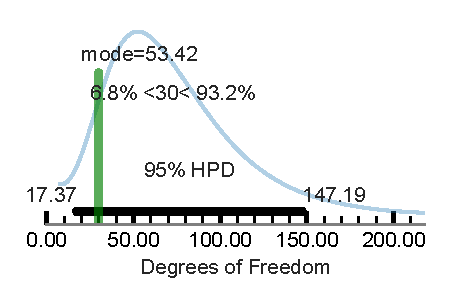
\includegraphics[width=0.5\textwidth]{./figures/robust_normality_font_fixed.pdf}
    \caption{The posterior distribution for $\nu$, the normality parameter of the $t$-distribution. When $\nu=\infty$ the $t$-distribution is identical to the Normal distribution. The posterior distribution shows a vertical green bar for $\nu=30$, the traditional cut-off condition on degrees of freedom, for using a Normal distribution. The mode $\nu=53.42$, and the posterior probability distribution implies that only about 7\% of the posterior lies to the left of the green line (i.e. $P(\nu \leq 30) \approx 0.07$), implying that the assuming that the likelihood function to be Normally distributed will give similar inference.}
    \label{fig:normality}
\end{figure}

% Having discussed posterior-prediction checks, model convergence, and normality, next, we discuss alternatives to the model.

% \subsection{Alternative Models}
% \label{sub:Alternative Models}

% As a first instance, consider a similar model, except that the scale parameter of the likelihood function is \textit{not nested} like our current model. Instead, we consider the equal variance case, where all the variances are equal (similar to ANOVA), and that the variance is drawn from a uniform distribution. In other words, $\sigma_j = \sigma \sim U(L, H)$, where $L>0$ and where $H$ is a large constant. The main effect of the equal variance assumption is that there is no information sharing among the groups as would be the case when each $\sigma_j$ is drawn from the same distribution, whose parameters have hyper-priors; the latter is our current model.

% The main effect of constraining our simplified model is that we are slightly poorer in predicting the observed data since all the variances are guaranteed by the model to be equal, whereas we can see from~\Cref{fig:traceplot} that the mean scale (or equivalently variance) in the text condition is lower. We are skipping the traceplot and the contrast plots in this case, as they are similar, to~\Cref{fig:traceplot} and~\Cref{fig:robustcontrasts}, except that the effect size for the combined case is slightly lower due to the equal variance assumption. 

% Instead, we compare the two models using WAIC (Widely Applicable Information Criterion), a principled way to compare models when they have identical likelihood functions~\parencite{Gelman2014a}. WAIC uses the predictive loss to compare two models with different parameters. First, WAIC computes the average log likelihood of each training data point (over the posterior distribution) less the variance of the log likelihood for the same data point; and then it computes the sum over all data points. That is, WAIC for a model: 

% \begin{equation*}
%     \mathrm{WAIC} = -2 \left (\sum_i^N \log \mathrm{Pr}(y_i) - V(y_i) \right) 
% \end{equation*}

% where, $N$ is the total number of training points, $y_i$ is the observation, $\mathrm{Pr}(y_i)$ is the averaged data likelihood over the posterior, and where $V(y_i)$ is the variance of the data likelihood over the posterior. When we compare the two models, one with unequal variances, and one with equal variances. We show our results in~\Cref{tab:WAIC comparison}:

% \npdecimalsign{.}
% \nprounddigits{2}

% \begin{table}[htb]%\footnotesize
%     \centering
%         \caption{WAIC comparison between the model with equal variances against the case when the variances are not constrained to be equal (i.e. we use a hierarchical model). Both cases assume the Student-$t$ likelihood function, the function used in this paper. The columns show respectively, WAIC, pWAIC (the effective number of parameters; also: $\mathrm{pWAIC}=\sum_i V(y_i)$), dWAIC (the difference between the WAIC scores of the other models with the best model), weight (the relative probability that the model explains the data) SE, the standard error of the WAIC estimate, dSE is the standard error of the difference of the current model against the top model. The table shows that the hierarchical model with unequal variances better explains the observations. }\label{tab:WAIC comparison}
%         \begin{tabular}{rcccccc} \toprule
%             Model & WAIC & pWAIC & dWAIC & weight & SE & dSE \\ \midrule
%              Unconstrained variances, hierarchical    & 1102.48    & 3.95 &     0.00 &     1.00 &     14.61 &     0.00    \\
%             Constrained, equal variances & 1104.17 & 3.42 & 1.69 & 0.00 & 14.25 & 1.54        \\ \bottomrule
%         \end{tabular}
    
%     \end{table}

% The results in~\Cref{tab:WAIC comparison} say that model with the unconstrained variances is better at explaining the data than the model with constrained variances; the relative probability that the hierarchical model with unconstrained variances better explains the observation is 1.0 (refer to the weight column in~\Cref{tab:WAIC comparison})

% How useful was the choice of the Student-t drawing distribution~\Cref{eq:bayesian formulation}, instead of assuming that the outcomes are drawn from a Normal distribution? Our analysis of the posterior distribution of the degrees of freedom parameter $\nu$ shows that there is only a small probability ($P(\nu \leq 30) \approx 0.07$) that $\nu \leq 30$. Thus, we may use the Normal likelihood function, without meaningfully affecting the conclusions. Indeed, in our experiments, when we do model the observations with a Normal likelihood, assume equal variances, we find no meaningful differences in the contrasts or the effect sizes, with the Student-$t$ model with equal variances (results omitted due to space constraints).

% Since the charitable donations are bounded to lie between \$0.0 and \$5.0, might we benefit from using bounded likelihood functions like the Beta distribution $Y \sim Beta(\alpha_j, \beta_j)$ to represent the charitable donations $Y_j$ under the different conditions $j$? While a $Beta(\alpha, \beta)$ distribution lies between $[0,1]$, we can scale down the contributions to lie in $[0,1]$ to use with the $Beta(\alpha, \beta)$ distribution. But notice from~\Cref{fig:contributions across conditions} that in each experimental condition, there is a central lobe, and heavy tails at each extreme, notably at \$0.0 and at \$5.0. 

% Our view of models motivated by~\textcite{McElreath2015} is that they represent an \textit{epistemological} claim, not an \textit{ontological} claim (i.e. a physical assumption about the world). Since our goal is to understand the average tendency to give to charity under the different conditions, and not to make predictions (as might be the case if we were trying to model donation with age as a predictor), the fact that the $t$-distribution is not bounded is less relevant here. 



Our posterior predictive check shows that the $t$-distribution models well the heavy tails, and shows that the variances for the comic conditions are different from the text condition. Furthermore, the comparison between the hierarchical model with unconstrained variances and the model with equal variances shows that the hierarchical model is better at explaining the observations. We discuss posterior prediction checks (\Cref{sub:Posterior Predictive Check}) and alternative models (\Cref{sub:Alternative Models}) in detail in the Appendix. 

To summarize, we discussed transparency and utility in small-$n$ studies as motivation for our use of Bayesian modeling. The model shows good convergence with the Gelman-Rubin statistic $\hat{R}$ was virtually identical to 1.0 for all parameters; the effective sample size was greater than 10,000 for all parameters. The modal value of $\nu$, the degrees of freedom parameter was around 53, suggesting that we could also use the Normal likelihood function. 

%!TEX root = cscw2019-comic.tex
\section{Discussion}
\label{sec:Discussion}
We will first summarize our findings and discuss experimental variations. Then, we will propose a framework for algorithmically synthesizing persuasive messages into the abstract comic form, discuss design implications, and identify limitations.

\subsection{Experiments: Findings and Alternative Contexts}
\label{sub:Experiments: Findings and Alternate Contexts}

From asking individuals to act to appealing for charitable donations, text messages have been widely used in simulating behaviors. Scholars from psychology have shown how variations in the construction of text messages alter decisions. We explored and examined the role of the abstract comic form, a highly expressive, affective medium in communicating persuasive messages. To test the effectiveness of abstract comic persuasive messages, we persuaded individuals to make online charitable donations, a common public good dilemma. In the dilemma, due to the non-exclusive and non-rivalrous nature of public goods, persuading individuals to contribute is hard and crucial. Also, online charitable donation task not only avoids confounding factors such as habit formation which exists in other persuasion tasks such as exercise and healthy diet but also assures the ecological validity of our study as charity and organizations often solicit donations online. In our study, we compared the persuasive power of text messages, comic messages, and comic messages with social proof in asking charitable donations to public health research (e.g., the Organization for Autism Research).

\begin{description} [leftmargin=\parindent,topsep=0pt,partopsep=3pt,parsep=0pt,itemsep=3pt, listparindent=\parindent]
    \item[Comic vs. Plain Text:] Our results show that study participants prefer persuasive messages in abstract comic form over plain text. When making the charitable donation between $\$0$ to $\$5$, study participants donated $\$ 0.86$ more if they read the persuasive message in an abstract comic form (see~\Cref{fig:robustcontrasts}, fourth column). The results demonstrate the persuasive power of abstract comic in stimulating behaviors in pro-social decisions. Our findings are consistent with prior research on visual stimuli in persuasion and the benefits of comics in communication. One potential explanation is that study participants were more attracted by the comic strip and projected themselves onto the character. When the projection happens, the persuadee may be able to digest the information better which stimulated them to donate more to the Organization for Autism Research. 
    
    \item[Social Proof Condition:] When comparing between the comic condition and comic with the social proof condition, although study participants who read the comic with social proof donated more on average (\$0.19 more) that the comic only condition, our analysis results do not indicate a significant difference between the two conditions (see~\Cref{fig:robustcontrasts}, third column). 
    % Although the use of social proof showed a significant impact on other forms of persuasive messages (e.g., plain text), in the abstract comic messages, the effect is not substantial. 
    We can identify two explanations. First, it is possible that the design of our comic strip did not signify the idea of social proof strongly---we simply introduced the pilot study statistic in the text bubble. Other comic designs, e.g., adding other donators as comic characters, may make the social proof more salient. Another potential explanation is that the influence from other study participants is not strong enough. As \textcite{goldstein2008room} discovered hotel towel re-use study, stronger the relationship between the subject and the reference group of individuals from whom the experimenters compute the statistic for the social norm, the message is more persuasive. It is possible that the relationship between the AMT subjects may be weaker than the study in \textcite{goldstein2008room}'s towel re-use study.

    We conjecture that using a person's social network as part of the social proof (after seeking consent, for example, to use the person's Facebook profile information) may increase the contribution, but needs further research. We know from Cialdini's seminal work on persuasion that knowledge of friends performing similar behavior is persuasive. We know from \textcite{small2007sympathy}'s work on charitable donation that named entities are more powerful in persuasion than abstract statistics (e.g. ``Jane Doe is a hurricane survivor; please help'' vs. ``3000 people homeless due to the hurricane; please help''). If the person has given consent, a charity could find out in real time, the Facebook friends of the person who has loaded the web-page, and compute the fraction who have donated and use that number in the social proof. Or to use tie-strength \cite{Gilbert}, if available and name the closest friend who has donated to the charity, in the social proof message. However, we know from recent work \cite{eslami2018communicating} that when advertisers display information that subjects find ``creepy'' (as demonstration of knowledge by the charity of the subject's closest friend, of even statistics of the person's Facebook friends circle contributions), the subjects may find the charity less trustworthy and may donate less.
    
    % discovered that the closer the relationship is, the stronger the social proof will be, comparing to the neighbors or people stayed at the same room in \textcite{Cialdini2004} and \textcite{goldstein2008room}'s work, the relationship among participants in our study may be much weaker. So, we did not observe a strong influence from abstract comics with social proof.
    \item[Donation Amount:] Another natural question to ask is whether the maximum donation amount of  \$5  in our study has any influence on our findings (e.g., will people make the same donation decision if they can donate more?).  Prior studies in behavioral economics suggested that small-stake experiment in developed countries can be replicated in developing countries where the stake becomes a significant portion of participants' weekly income \cite{binswanger1980attitudes,binswanger1981attitudes,kachelmeier1992examining}. Additionally, \textcite{post2008deal} showed that the results from small-stake experiments would hold with higher stakes in developed countries as well. Those results seem to suggest that our findings will hold with higher donation amount. However, the best way to confirm is through actual experiments. 
    \item[Other Media Forms:] While a direct comparison between the comic form and images and videos is beyond the scope of the paper, we discuss two advantages of using the abstract comic to persuade.There are two points to consider: the ease of making a connection with a viewer (the abstract comic form vs. images or video); infrastructure to create tailored messages. First, as \textcite{mccloud2011making} points out, when using the abstract comic form, the reader projects themselves onto the character. A concrete and detailed representation of the person in the comic causes the reader develops a sense of the ``other'' - that is, they are viewing someone else enacting a scene. Using images and videos with actual human models, will create a sense of the ``other'' for the viewer, and then the images/video need to connect with the viewer through demographic, cultural and local cues. For example, in advertising, to allow for recipients of ads to identify with the message context, advertisers try to ensure that the models who appear in images match the target demographic. In contrast, when viewing an abstract comic, the reader fills in the gaps with their own characteristics, and they see themselves as the protagonist. Second, our infrastructure (discussed next in~\Cref{sub:framework}) makes it straightforward for a charity to compose a multi-panel abstract comic. The infrastructure to create tailored imagery and videos may be expensive for the charity. Today, advertisers tailor the imagery (usually the individual in the image) in online banner ads (embedded on a web page) to the demographics of the person viewing the ad. Matching the demographics requires that advertisers access the information stored in a browser cookie against third-party information about the person in real-time. This real-time switching of imagery is expensive: it requires a manually curated image collection corresponding to individuals matching to different demographic segments of interest. And, to personalize the message (e.g. with the social norm), they would need to have the infrastructure to compose the message on the fly. Furthermore, algorithmic synthesis of persuasive, personalized videos is more challenging. One possibility that we do consider as part of future work: animations that involve the abstract comic form.
    %\textcolor{red}{When considering persuasive messages in non-textual forms, besides abstract comics, graphical representation and video messages are often discussed. Although the scope our study is not to compare the persuasive power between comics and other non-textual forms, the abstract nature of the comics allows low-cost synthesizing comparing to other non-textual forms, especially when the original message is personalized, which makes the abstract comic persuasive message worth to consider.}
    \item[General Experimental Flow:] Consider three online charitable donation scenarios related to how the charitable organization knows the person asked to make a donation. In each case, consistent with prior work ~\cite{pessemier1977willingness}, the charity needs to establish context. There are three ways to consider.
    
    First, the person may be familiar with the charity through their lived experience. For example, in the case of Wikipedia, the person may be someone who uses the site frequently. A person who regularly uses the Wikipedia site is unlikely to need a video describing Wikipedia benefits. In such cases, we envision using the three-panel comic instead of the desktop banner ad that Wikipedia uses at the moment.
    
    Second, the person may be a member of the charity or non-profit (e.g. museums).For 501(c) non-profit organizations with memberships, that recognize that a member has logged onto the organization website, again detailed context may be less necessary and they could use the three-panel comic along with their regular ask page, along with social proof describing the fractions of other members who have contributed.
    
    Third, the person may not know the charity. For charities who need to ask for donations without the benefit of either lived experience or of memberships, need to establish context from scratch. They may establish context through videos, a page with text and images or even a physical mailer. After watching the videos or reading the page, they may show the person visiting the page the comic. For the physical mailer, the charity would include its usual textual description and imagery followed by the abstract three-panel comic. After the comic panel, they may direct the person opening the mailer to a web-page to make a contribution.
    
    For the first two scenarios, a charitable organization (e.g. Wikipedia) can determine regular use of its website or determine if the person visiting the web-page is an organization member through the use of advertising cookies.

    
    %\hs{How might a charity use our findings? In general, consistent with prior work on donations~\cite{pessemier1977willingness} that indicates that an individual's prior knowledge of the purpose may influence their donation behavior, the charity first needs to establish common grounding with a potential donor and then make the request. In the present study, the video plays helps the experimental subjects familiarize themselves with the charity. The role of the video is to provide context, grounding the subject with the purpose of the charity. } 
    
    %\hs{In general, a person may establish grounding with the charity in other ways beyond an introductory video or a web-page with descriptions, including through their lived experience and through membership. Consider two examples. First, a person who regularly uses the Wikipedia site is unlikely to need a video describing Wikipedia benefits.  In such cases, one may envision using a multi-panel comic instead of the desktop banner ad that Wikipedia uses at the moment.  Second, for 501(c) non-profit organizations with memberships (e.g. museums), that recognize that a member has logged onto the web-site, again detailed context may be less necessary and they could use the three panel comic along with the regular ask page, along with social proof describing the fractions of other members who have contributed.  A charitable organization (e.g. Wikipedia) can determine regular use of its website or determine if the person visiting the web-page is a organization member through the use of advertising cookies.} 
    
    %\hs{For charities who need to ask for donations of an individual without either experience with the charity or is not a member, the charity needs to establish context. They may establish context through videos, a page with text and images or even a physical mailer. After watching the videos or reading the page, they may then show the person visiting the page the comic. For the case of physical mailer, the charity would include its usual textual description and imagery followed by the abstract multi-panel comic. After the comic panel, they may direct the person opening the mailer to a web-page to make a contribution.}
\end{description}




% \textcolor{red}{We conjecture that using a person's social network as part of the social proof may increase contribution, but needs further research. We know from Cialdini's seminal work on persuasion that knowledge of friends performing similar behavior is persuasive. We know from \textcite{small2007sympathy}'s work on charitable donation that named entities are more powerful in persuasion than abstract statistics (e.g. "Jane Doe is a hurricane survivor; please help" vs. "3000 people homeless due to hurricane; please help").It ought to be straightforward for a charity to find out in real time, the Facebook friends of the person who has loaded the web-page, and compute the fraction who have donated and use that number in the social proof. Or to use tie-strength \cite{Gilbert}, if available and name the closest friend who has donated to the charity, in the social proof message. However, we know from recent work \cite{eslami2018communicating} that when advertisers display information that subjects find "creepy" (as demonstration of knowledge by the charity of the subject's closest friend, of even statistics of the person's Facebook friends circle contributions), the subjects may find the charity less trustworthy and may donate less.}

% Another natural question to ask is whether the maximum donation amount of  \$5  in our study has any influence on our findings (e.g., will people make the same donation decision if they can donate more?).  Prior studies in behavioral economics suggested that small-stake experiment in developed countries can be replicated in developing countries where the stake becomes a significant portion of participants' weekly income \cite{binswanger1980attitudes,binswanger1981attitudes,kachelmeier1992examining}. Additionally, \textcite{post2008deal} showed that the results from small-stake experiments would hold with higher stakes in developed countries as well. Those results seem to suggest that our findings will hold with higher donation amount. However, the best way to confirm is through actual experiments. 

% \textcolor{red}{While a direct comparison between the comic form and images and videos is beyond the scope of the paper, there are two points to consider, when comparing the comic form, to images and video. First, the abstract comic form used in our experiment allows the reader to project themselves onto the comic character. Our infrastructure (discussed in section x) makes it straightforward for a charity to compose a multi-panel  abstract comic. We plan to make the infrastructure publicly available as open source software after publication,Second, to allow for recipients of ads to identify with the message context, advertisers like to ensure that the models who appear in images match the target demographic. Today, advertisers tailor the imagery (usually the individual in the image) in online banner ads (embedded on a web page) corresponding to the demographic of the person viewing the ad. Matching the demographic requires the advertisers to access the information stored in a browser cookie against third-party information about the person. This real-time switching of imagery is expensive: it requires a manually curated image collection corresponding to individuals matching to different demographic segments of interest. Furthermore, to personalize the message (e.g. with the social norm), they would need to have the infrastructure to compose the message on the fly. Furthermore, algorithmic synthesis of persuasive videos is more challenging.Thus, synthesizing personalized images and videos tailored to the individual may be expensive to generate for a charity. In contrast, they could use our open source software to create an abstract comic for persuasion.}
%\textcolor{red}{When considering persuasive messages in non-textual forms, besides abstract comics, graphical representation and video messages are often discussed. Although the scope our study is not to compare the persuasive power between comics and other non-textual forms, the abstract nature of the comics allows low-cost synthesizing comparing to other non-textual forms, especially when the original message is personalized, which makes the abstract comic persuasive message worth to consider.}

% Although in our study, the persuasive goal is making charitable donation decisions, we believe our findings suggest future research on longitudinal behavior change (e.g., health) via the abstract comic. 

 \subsection{Framework for Algorithmically Synthesized Abstract-Comic Persuasive Messages}
 \label{sub:framework}
 
Our study showed the persuasive power of abstract comics in encouraging people to make pro-social decisions. However, one drawback of using visual stimulus in persuasion is cost during the creation process. Although compared to creating other persuasive visual stimuli such as videos or complex graphical illustration, the simplicity of abstract requires less effort, the creation process is not easy. In this section, we propose a framework that allows full/semi- automatic generation of abstract persuasive messages and identify crucial features that need to be addressed in future work. We believe such a tool will lower the barrier for the persuader to take advantage of the abstract comic (as demonstrated in our study) in encouraging individuals to act in public good dilemmas.

In our study, we created a comic generator with existing packages including ``cmx.io'' \cite{cmx.io} and ``rough.js'' \cite{rough.js} to generate the three-panel abstract comic strip. With several pre-defined character gestures (see~\Cref{figur:figures}), the generator only requests the text input from the persuader to create the comic message.  

We believe the comic generator built in this study can be further developed as a framework for algorithmic synthesis. Now, we identify crucial features that need to be addressed in future research. First, the framework should be able to automatically select the character gesture that best fit the persuasive message's context. For example, when the message receiver was told good news, his/her gesture should reflect that conflict. The appropriate mapping will create a natural and coherent comic message which is the key for an expressive message. We need future research to realize such a method. Second, the framework should be able to use other abstract comic elements, such as inter-character distance and shading, to create persuasive comics. To achieve this feature, we need to understand how different elements affect the persuasiveness of the abstract comic messages. Third, the framework should be able to personalize the persuasive comics by using persuadee's behavioral data to inform comic contents. We could derive the statistics for the social proof from the behaviors of friends and the data from a person's own activity.

\begin{figure}[t]
    \centering
    \begin{tabular}{cc}
        \subfloat[Gestures for positive framed messages]{\label{figur:1a}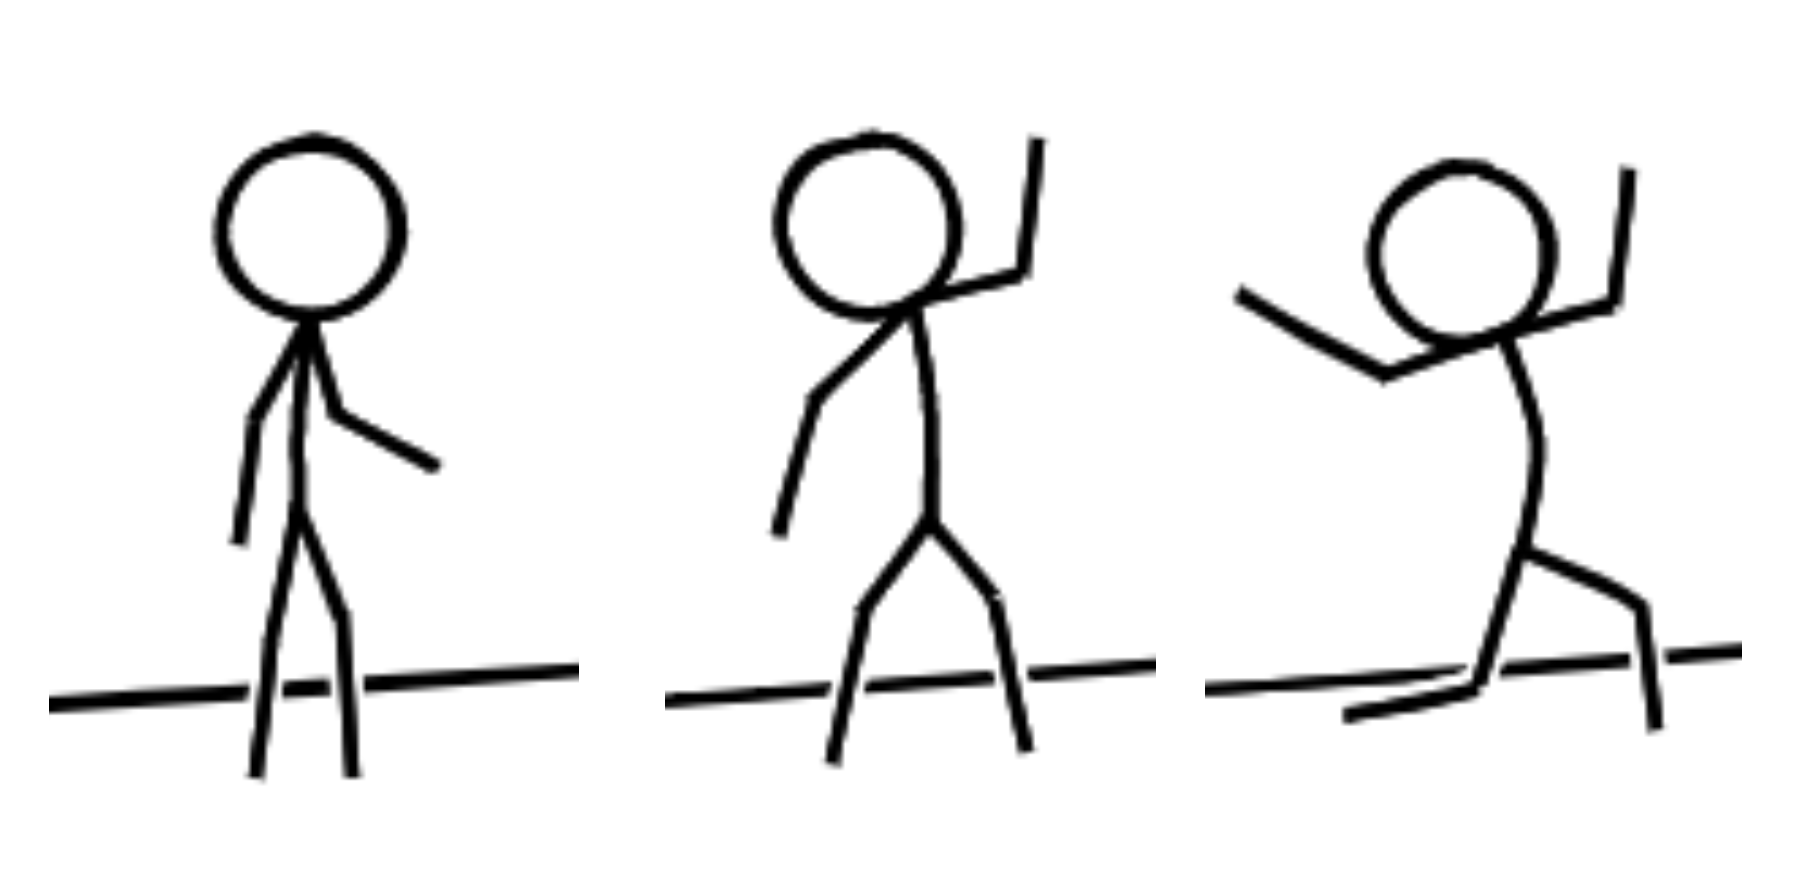
\includegraphics[width = 0.4\columnwidth]{figures/pos_figures}} &
        \subfloat[Gesture for negative framed messages ]{\label{figur:1b}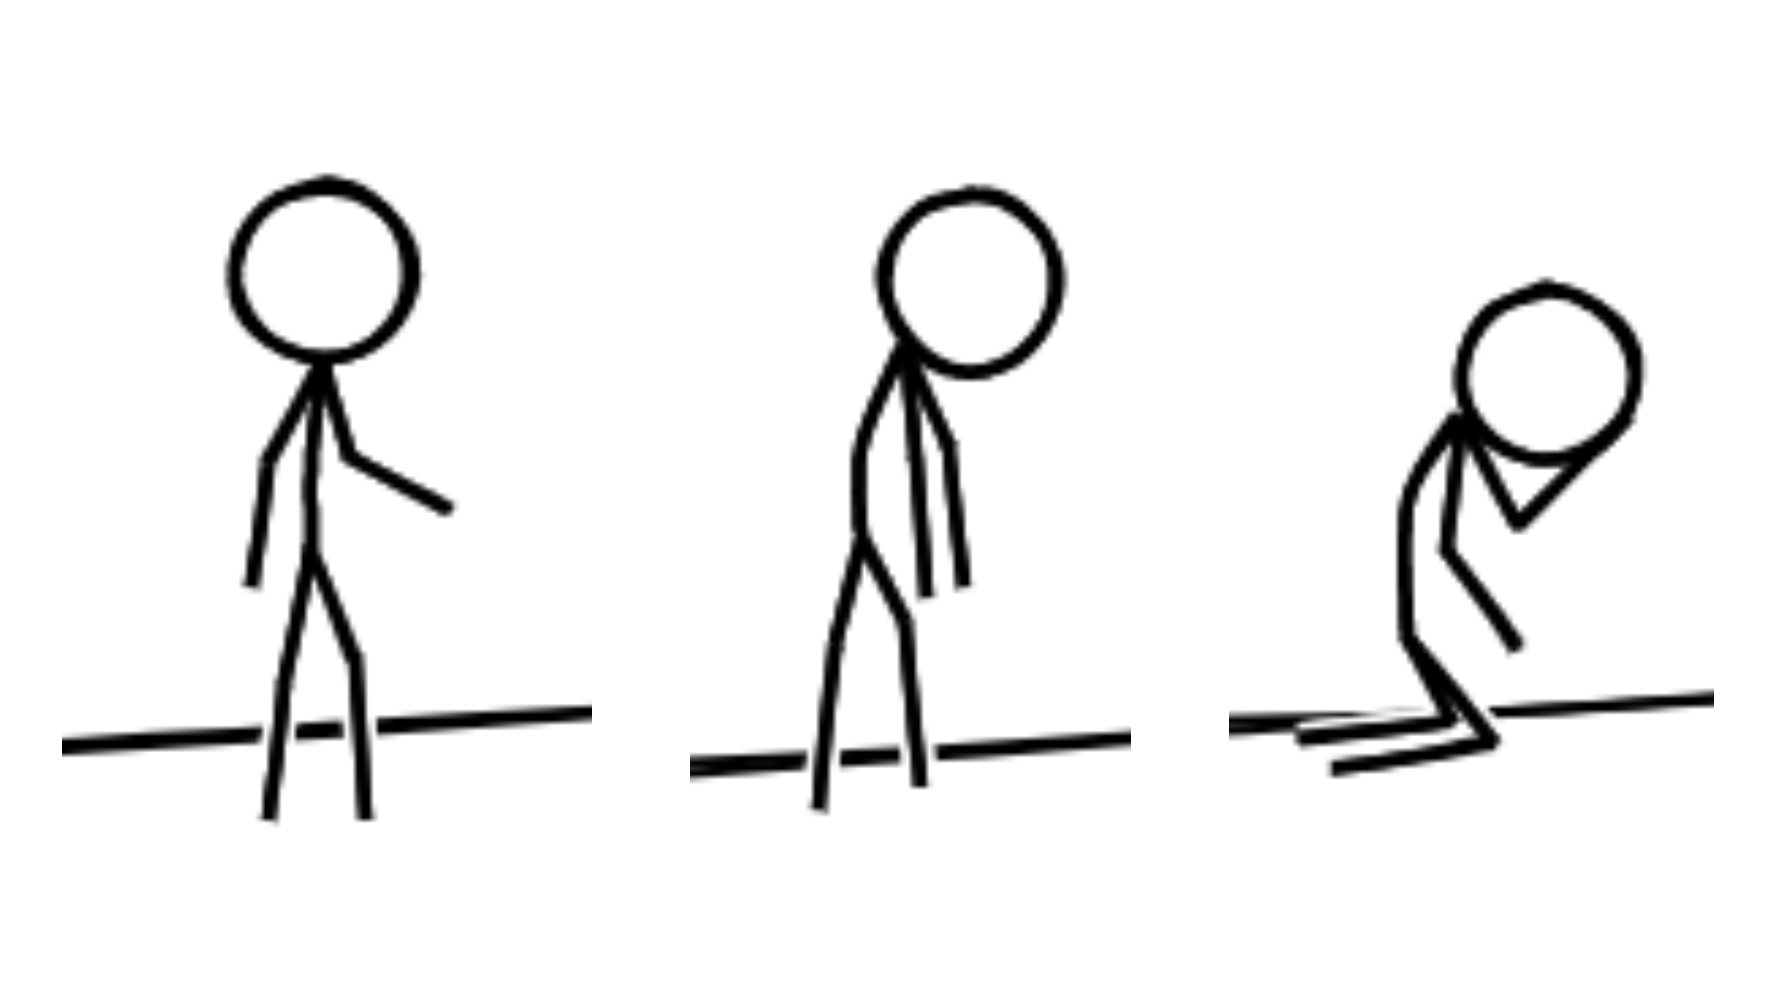
\includegraphics[width = 0.4 \columnwidth]{figures/neg_figures}}\\
    \end{tabular}
    \caption{Different character gestures to communicate various levels of emotional intensity. The left figure shows gestures from neutral to the happiest. The right figure shows gestures from neutral to the most frustrated. }
    \label{figur:figures}
\end{figure}

\subsection{Design Implications}
Our main design implications are two folded. First, when encouraging individuals to contribute to public goods, non-profit organizations and governmental agencies ought to consider to use abstract comic in their online messaging strategies to persuade. From our results, using abstract comics can, in particular, persuade people to act in public-goods dilemmas that require single-shot decisions (online charitable donations). Additionally, when constructing persuasive comics, it is worthwhile to consider to incorporate social norms. In the study, the purpose of the video is to inform participants about the context. Charities could use the comic after they've established context as discussed in~\Cref{sub:Experiments: Findings and Alternate Contexts}. 
% in the real world, the abstract comic message can be combined with campaign videos online to solicit donation.  Organizations can also consider to combine abstract comic messages with other introductory materials such as texts in an email or a physical mailer to persuade for contribution.

%; taking the flu shot
Second, our results also inform the development of a computational framework that can algorithmically synthesis textual persuasive messages into abstract comic form and uses data-driven methods to personalize the message to further increase messages' persuasive power. 
% With such a framework, agencies can create their abstract comic persuasive messages easily and incorporate them to alleviate real-world public goods dilemmas. 

\subsection{Limitations \& Future Work}
\begin{description}[leftmargin=\parindent,topsep=0pt,partopsep=3pt,parsep=0pt,itemsep=3pt, listparindent=\parindent]
\item[Distant and Non-exclusive Task:]  Although our study asked participants to make the decision with a real cost, the decision domain is limited to only one scenario, online charitable giving. In this task, the participant's reward is distant and non-exclusive (e.g., participant's donation decision won't bring any immediate reward and won't exclude the participant from the research outcome). Although both characteristics help us clearly test the persuasive benefits of abstract comics, they also limited our generalizability. We need future research to understand the pros and cons of using abstract comic messages in persuasive tasks with different reward characteristics. For example, for persuasive goals in the quantified-self movement~\cite{Epstein2014,Choe2014} such as exercise and dieting, the reward is distant (e.g., people's health won't be improved immediately after exercise) but exclusive (e.g., healthy life situation mainly benefit the individual him/herself). Moreover, our persuasion task is for an online charitable donation. Future work is needed to extend our result to offline charitable donation solicitation where persuasive text messages, such as mailers, also often used. 
\item[Study on Amazon Mechanical Turk:] We recruited our participants from Amazon Mechanical Turk, consistent with prior research \cite{lee2013does,saunders2016no,sussman2015framing,arechar2017turking,branas2018gender} that used Amazon Mechanical Turk subjects to study charitable donations. 


Although research shows that populations on Amazon Mechanical Turk are diverse and mirror the US population \cite{buhrmester2011amazon,behrend2011viability,berinsky2012evaluating}, there are concerns about Amazon Mechanical Turk's sample representativeness \cite{landers2015inconvenient,paolacci2010running}. One potential solution is to use panel population where the panel company claimed to offer a more diverse and representative sample.
However, this method also has concerns in that the researcher can not directly cross-validate the sample's representativeness we have to trust the company's assertion. Another solution is using stratified sampling, but it is challenging to classify every member of the population into a subgroup properly. 

Another limitation from use of Amazon Mechanical Turk subjects in our study is that prior research \cite{paolacci2010running,paolacci2014inside,kaufmann2011more} indicates that compared to other recruiting methods, study participants from Amazon Mechanical Turk are more sensitive to monetary rewards as monetary rewards are their prime motive for participation. 
% , compared to other recruiting methods, study participants from Amazon Mechanical Turk are more sensitive to monetary rewards. 
Since we ask our AMT study participants to donate from their own prospective rewards, we may see a lower average donation across all conditions, than for the population sample less sensitive to monetary rewards. An alternative sampling method we could consider in the future work is recruiting participants from our own social network. We conjecture that we may see higher average contributions in each of three conditions, since these participants may be less sensitive to monetary rewards than AMT participants. However, we need to carefully control for other potential confounding factors such as study participant's knowledge about our experiment goal. 
% What if we could recruit 
% such as the participant's own social network, we may expect a higher donation amount among all conditions. However, besides the potential sample representativeness problem (e.g. determining the size of participant's social network for the experiment), use of a social network introduces a confound: participants who are friends outside of the experiment may communicate outside of experimental communication channels.
% such sample may bring unexpected confounding factors such as their relationship with the researcher and knowledge about researcher's study topic. Additionally, \textcite{rzeszotarski2014estimating} showed that crowdsourcing may elicited higher quality results than friendsourcing on social networks

%  Prior research [51,50,32] indicates that compared to other recruiting methods, study participants from Amazon Mechanical Turk are more sensitive to monetary rewards as monetary rewards are their prime motive for participation. Since we ask AMT subjects to donate from their own prospective rewards, we may see a lower average donation across all conditions, than for the population sample less sensitive to monetary rewards.
  \item[Comic Message Construction:] In our study, we constructed the comic messages in the XKCD comic style. Although the XKCD style is easily recognizable, there are many different ways to create abstract comics.  Comic, as a creative art form, has rich semantics and vocabularies to communicate ideas \cite{scott1993understanding}. Out of necessity, we limited the complexity our comics strip (e.g., number of characters, gestures, and the number of panels). Future research is needed to explore and understand how other elements in the comic, for example, inter-character distance and character's gesture, affect the persuasiveness of the comic. Furthermore, while simplicity grants us the possibility to automate the generation process, future technology may allow us to generate more complicated persuasive abstract comics.
  
    \item[Other Experimental Contexts:] What are other contexts to which our study results may apply? Although our study examined charitable donation decisions, a single shot task with distant, non-exclusive rewards, certain health related tasks may be candidates to study next. Recent work by~\textcite{Bushar2017} on using SMS text messages to persuade pregnant mothers to take influenza vaccinations suggests that those who received the text messages were more likely to report taking a vaccination than those who did not receive a message. Further research is merited to determine if for this single-shot task, with exclusive, non-immediate reward, an abstract comic (e.g. embedded as a link in the SMS) succeeds in increasing vaccination rates for pregnant women over the plain text.
  
\end{description}

%need to update this part after the revision of RQ in the introduction
%Our experiment answers RQ-1 affirmatively in that comics are more persuasive than text, with a moderate effect of 0.33. Our answer to RQ-2 is that while the effect of no element is significant, shading and gesture show strong influence, but surprisingly inter-character distance is most effective when distance is large. For RQ-3, we show that negative messages are more influential than positive messages. We have developed a prototypical comic generator (answering RQ-4) that can be used in deploying comic messages.

%  \item[No interaction effects in the model]: Our model does not include any interaction effects. This is by design, since in the first study we have 54 experimental conditions making any analysis interaction effects difficult with our small observational study. The raw data suggest an interaction between shading and gesture, but given our limited dataset, there is little point in modeling this interaction. We plan to study interaction effects in future studies by limiting the number of main predictor conditions.
 %\item[Ecological Validity:] There is a legitimate question if our experiment on Amazon Mechanical Turk has ecological validity.  In real life, many factors affect a person's decision, such as where they are and who they are interacting with. Those factors may interact with the abstract comic's persuasiveness. However, these concerns are also present in other standard studies conducted in the more familiar lab experiments. We plan to conduct field studies in real-world contexts (e.g., shopping at a grocery store) to explore this issue.

% followed Our analysis shows that subjects prefer persuasive messages in comic form over plain text. We found in a persuasive comic, different character's gestures and background shading can influence subjects' perception of the persuasiveness whereas no strong effect was found in inter-character distance. This was consistent with previous research on visual stimulus in persuasion and the benefits of comics in communication.
%
% \subsection{Inter-Character Distance}
% \label{sub:Inter-Character Distance}
% There may be two explanations to the odd result that the farthest distance between the two characters was more influential.
% % However, previous studies on comics composition suggests the inter-character distance can affect reader's perceived relationship between characters and therefore influence their perception of the persuasive comics.
% First, it may be the case that the subjects did not project themselves onto the comic as one of the characters and did not recognize the distance between characters as reflecting closeness of the relationship. For example, a subject may read the comic from a third-person narrative. We looked into some feedbacks from in the pilot study. One participant ($p_1$) mentioned \textit{``I really like the comic I just saw and I feel bad that someone told me ...''} which suggests the subject does think that they are in the comic and having a conversation with someone else. Yet, we don't know if they perceive their relationship with the persuader based on the inter-character distance. A second explanation is that closer inter-character distance causes a cluttered visual composition and thus the subjects perceive these comics as less visually pleasing.

% \subsection{Comics with Color}
% \begin{figure}[t]
%  \centering
%  \begin{tabular}{ccc}
%   \subfloat[Colored Text]{\label{figur:3o}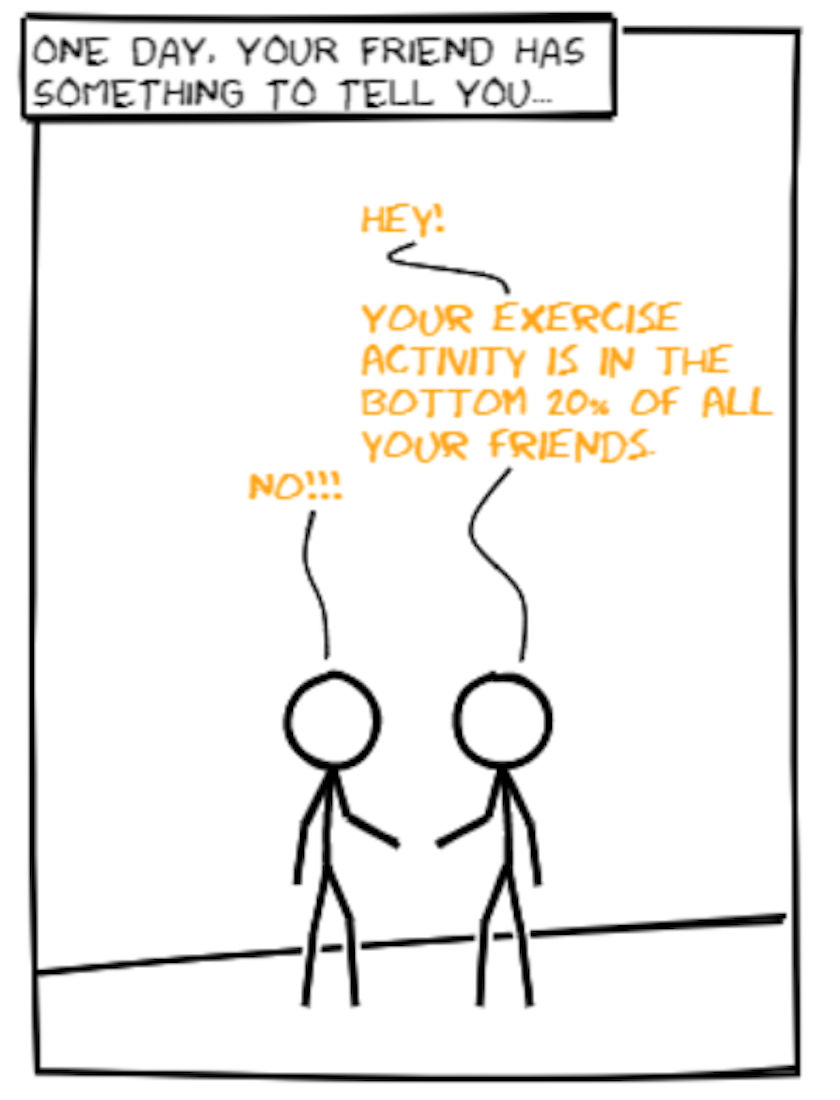
\includegraphics[width = 0.27\columnwidth]{figures/o1}} &
%   \subfloat[Colored Ground Line]{\label{figur:31}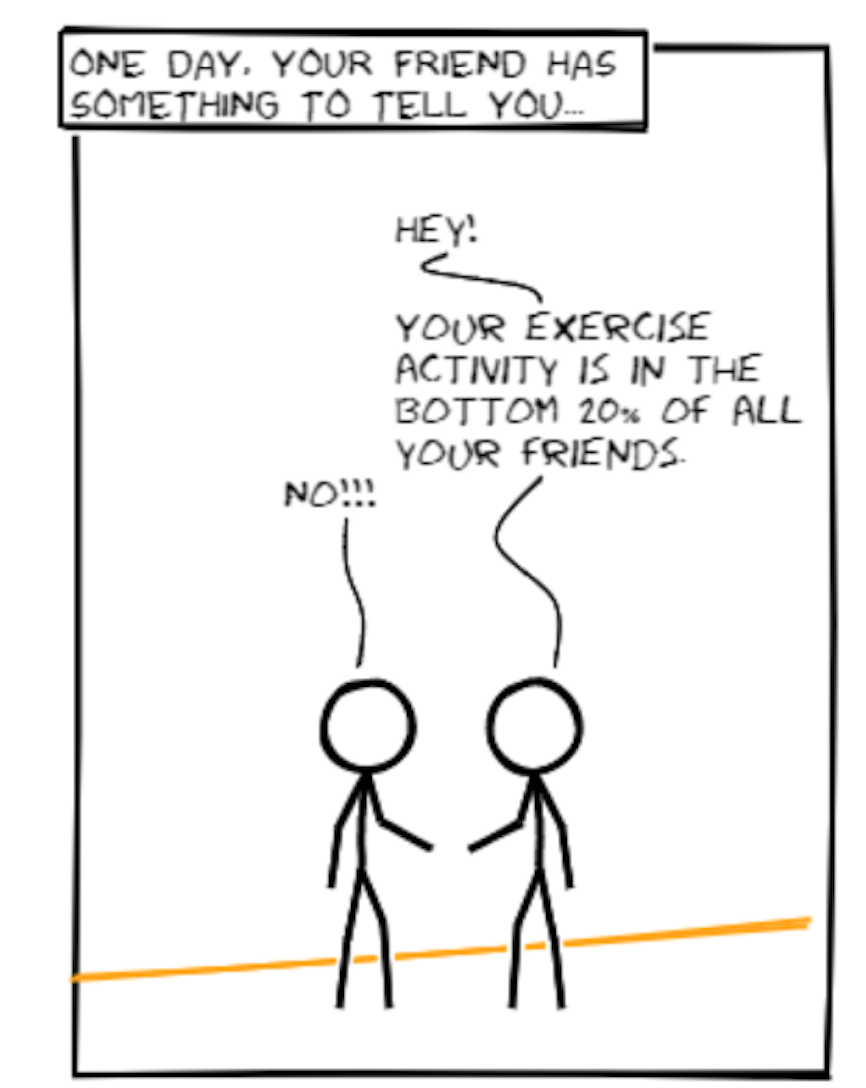
\includegraphics[width = 0.27 \columnwidth]{figures/o2}}      &
%   \subfloat[Colored Figure]{\label{figur:32}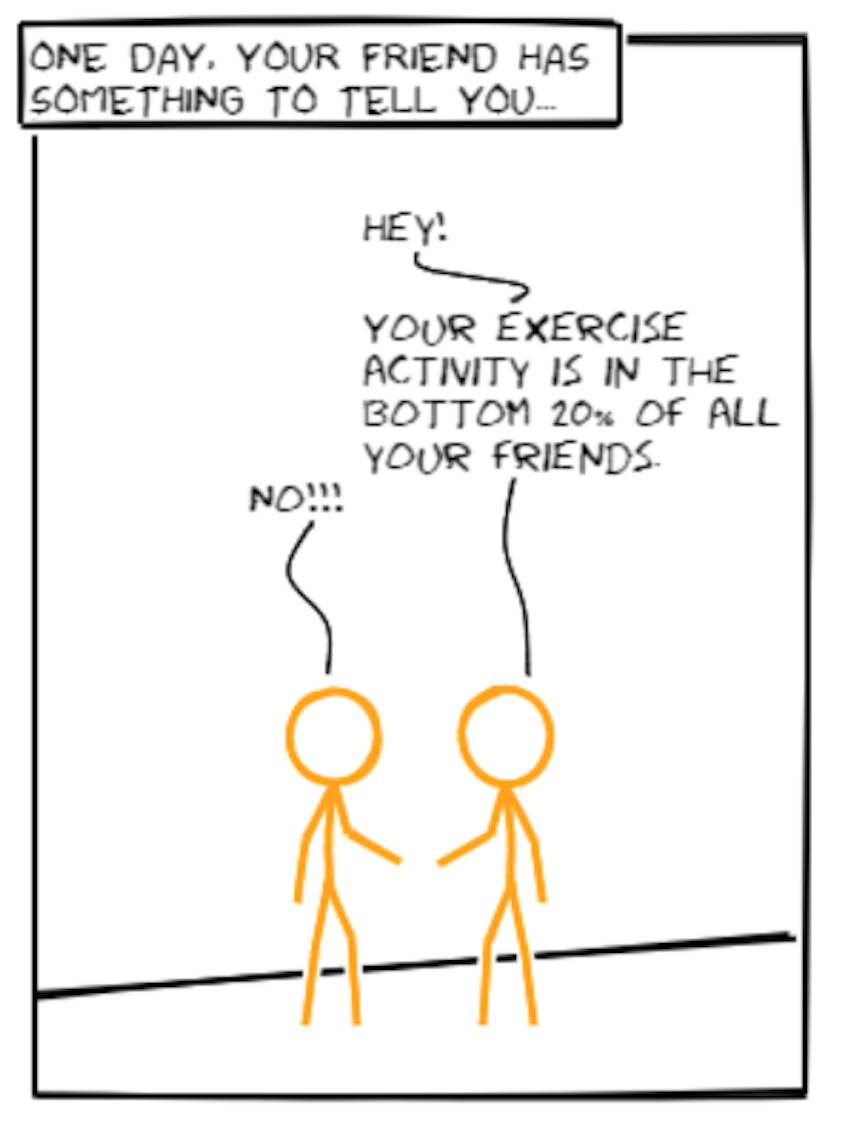
\includegraphics[width = 0.27 \columnwidth]{figures/o3}}\\
%  \end{tabular}
%  \caption{Colored different elements in a comic}
%  \label{figur:color}
% \end{figure}
%
% Our model suggests the background shading in a persuasive comic affects its persuasive power which makes us wonder the role of color as previous studies suggest the usage of color communicates the emotional intensity similar to the background shading. We ran a small scale study comparing the perceived persuasiveness between black-white comics in our study and their corresponding colored version,see figure~\ref{figur:color}. With 60 participants from the Mechanical Turk,  we found using an identical hierarchical Bayesian formulation that our subjects perceive colored version as more persuasive and there is potential interaction effect between negative-positive framing and different colors (see~\Cref{fig:color-experiment-effect}). We plan to run larger experiments that include color and study the interaction with framing and other elements.
%
% \begin{figure}
%  \subfloat[The mean effect and the effect size with color\label{subfig-1:color-mean-effect}]{%
%   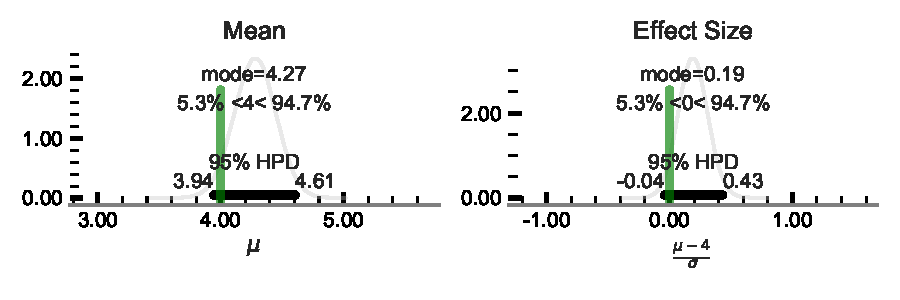
\includegraphics[width=0.6\textwidth]{./hari-code/factors_mean_effect_color-no-interaction.pdf}
%   } \hfill
%  \subfloat[Color contrast\label{subfig-2:color-contrast}]{%
%   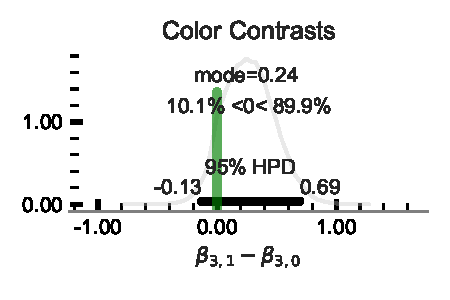
\includegraphics[width=0.33\textwidth]{./hari-code/factors_color_contrasts_color-no-interaction.pdf}
%  }
%  \caption{~\Cref{subfig-1:color-mean-effect} shows the High Posterior Density (HPD) intervals for the mean response $\mu$ and effect sizes $\sigma_y$ in the presence of color. HPD represent the region with 95\% of the density. Notice that the HPD interval for $\mu$ is $[3.94, 4.27]$ and includes a ROPE of $[4\pm 0.1]$ (the interval includes 4, the neutral response value). Thus while there no significant effect, we note that nearly 94\% of the HPD lies to the right of 0. The figure for effect size shows a small effect with mode $0.19$; since the HPD interval $[-0.04, 0.43]$ includes a ROPE of $[0\pm 0.1]$, there is no significant effect.~\Cref{subfig-2:color-contrast} shows the contrasts between the use of the two colors. The modal value is $0.24$, but since the HPD interval $[-0.13, 0.69]$ overlaps with 0, there is no appreciable effect (but notice that 89\% of the density lies in the region greater than 0.)}
%  \label{fig:color-experiment-effect}
% \end{figure}


%  Large scale field study is needed to demonstrate how the abstract comic can persuade in the real-life decision making and what will affect its persuasiveness.
 %Since we ask the subjects (who may lack interest in exercise) to evaluate persuasiveness when the topic is on exercise. Notice that our goal is not to persuade experimental subjects to exercise more, but to evaluate if the comic is a more persuasive form of communication of a statistical fact. We should expect---since we don't know if the subjects are interested in exercise---an increase in the variance in the estimates of the parameters (in particular,  $\sigma_y$). Despite this, the analysis shows a significant affirmative result for RQ-1.
%  \item[Appropriate gestures]: The authors determined gestures used by the characters in the experiment through trial and error. It may be useful to examine  theoretical frameworks from dance as well as theater art forms as well as examine work on design of sign languages.
% \end{description}
 % \item[Single Panel]: Our experiment limits our comics to a single panel which hinders one of the most fascinating aspect of comics---storytelling. Comparing to the comic strip, single panel comics find it harder to show the dynamic among characters.

%The main implication of our study lies in how to deliver persuasive messages. 

%Given the increasing popularity of wearable devices including smartwatches, one could consider presenting persuasive messages in the form of an abstract comic, where the three-panel comic is shown in sequence, perhaps even in animation. 

%Also, ~\textcite{scott1993understanding} identifies several fundamental components that influence reader reaction: character gestures, inter-character distance, and shading intensity. For example, the gesture of a character can help the reader to understand the interaction between characters and the emotion of the character. As a common technique, cartoonists often use the gesture to intensify the feeling that they want to communicate to the reader \cite{scott1993understanding}. Therefore, one of the future direction should be understanding how the different comic components moderate comic persuasiveness. If different comic elements car persuades differently, taking advantage of data-driven methods, the abstract-comic can better persuade. To maximize the persuasive power, future research on computational persuasion should leverage the receiver's personal model to construct the persuasive abstract comics with elements best fit to the persuadee.

%!TEX root = cscw2019-comic.tex
\section{Conclusion}
\label{sec:Conclusion}

Inspired by a rich history in persuasive test messages construction and benefits of abstract comic in communication, this paper examined if the abstract comic form was more persuasive than the corresponding plain text in the context of encouraging participants to donate for charitable causes. We conducted a field study on Amazon Mechanical Turk with 307 participants. In the study, participants received one of the three persuasive messages designed to ask for a donation to the Organization of Autism Research, a persuasive text message, a three-panel comic strip, and a three-panel comic strip incorporating the idea of social proof, and made donation decisions with real money. We analyzed the results using a hierarchical Bayesian framework that allows for understanding effect sizes, as well are transparent and helpful in small-$n$ studies. The results shows convincingly that the three-panel abstract comic is more persuasive than the text (a medium to large effect size = $0.59$). We also show that while the comic with social norm increases the donation level over the comic without the norm, the effect size is very small ($0.11$) and the increase is not meaningful. To summarize, the comic form meaningfully increases donations over the plain text, but the presence of the norm is not effective. We caution that the result holds for single-shot, public goods tasks; the value of the social norm in the comic, for exclusive tasks with distant rewards such as exercise, or dieting needs future research. The main implication of our work is that non-profits and Governmental agencies ought to consider using abstract comic in their online campaign as they work to alleviate public goods dilemmas. We believe that these agencies can easily include the use of the comic form as part of their overall messaging strategy because the simplicity of the abstract comic form allows it to be easily synthesized and to additionally incorporate social norms. 

As next steps, we plan to develop an algorithmic framework that automatically maps a person's behavioral data (e.g. amount walked this week) to a three-panel persuasive comic. We also plan to conduct longitudinal field experiments with an emphasis on storytelling where individuals receive three-panel comics over time, and comics are connected with a storyline.

%The main implications of our work lie in how persuasive messages are delivered, especially to wearable devices. As next steps, we plan to develop an algorithmic framework that automatically maps a person's behavioral data (e.g. amount walked this week) to a three-panel persuasive comic. We also plan to conduct longitudinal field experiments with an emphasis on storytelling where individuals receive three-panel comics over time, and comics are connected with a storyline.


%Three ideas were key to our work: the role of abstract comics to allow readers to project themselves onto the comic and ``social proof'' (that we adopt the decisions from other donaters) .


%The study on charitable giving examined if the abstract comic form was more persuasive than text. We analyzed the results using a hierarchical Bayesian framework that allows for understanding effect sizes, as well are helpful in small-$n$ studies. The results shows convincingly that the three-panel abstract comic is more persuasive than the text (medium effect size=0.44). The presence of the social proof is also effective, but provides only a minor improvement to the use of the abstract comic (effect size =0.12; not a meaningful improvement). The main implications of our work lie in how persuasive messages are delivered, especially to wearable devices.

% comics have a significant but moderate effect (effect size: 0.33) on persuasiveness compared to text. While no comic element has significant effect, we can observe that non-neutral gestures and shading as well as negatively framed messages have a strong influence. We conducted a smaller study with color and the result indicates that color too has a strong influence. Finally, we developed an abstract comic panel generator that takes as input the different comic elements, the valence of the frame and the message. We plan to release the code for Bayesian analysis and comic generator and the raw data under an appropriate open source license.


%!TEX root = cscw2019-comic.tex
\section{Acknowledgements}
\label{sec:Conclusion}
We thank all participants who joined our study. We are also grateful to reviewers for their insightful feedback. 

\printbibliography
%!TEX root = cscw2019-comic.tex
\section{Appendix}
\label{sec:Appendix}
% \section{Model Criticism}
\subsection{Posterior Predictive Check}
\label{sub:Posterior Predictive Check}

In this section, we examine how well our model makes predicts the observed data.

\begin{figure*}[htb]
    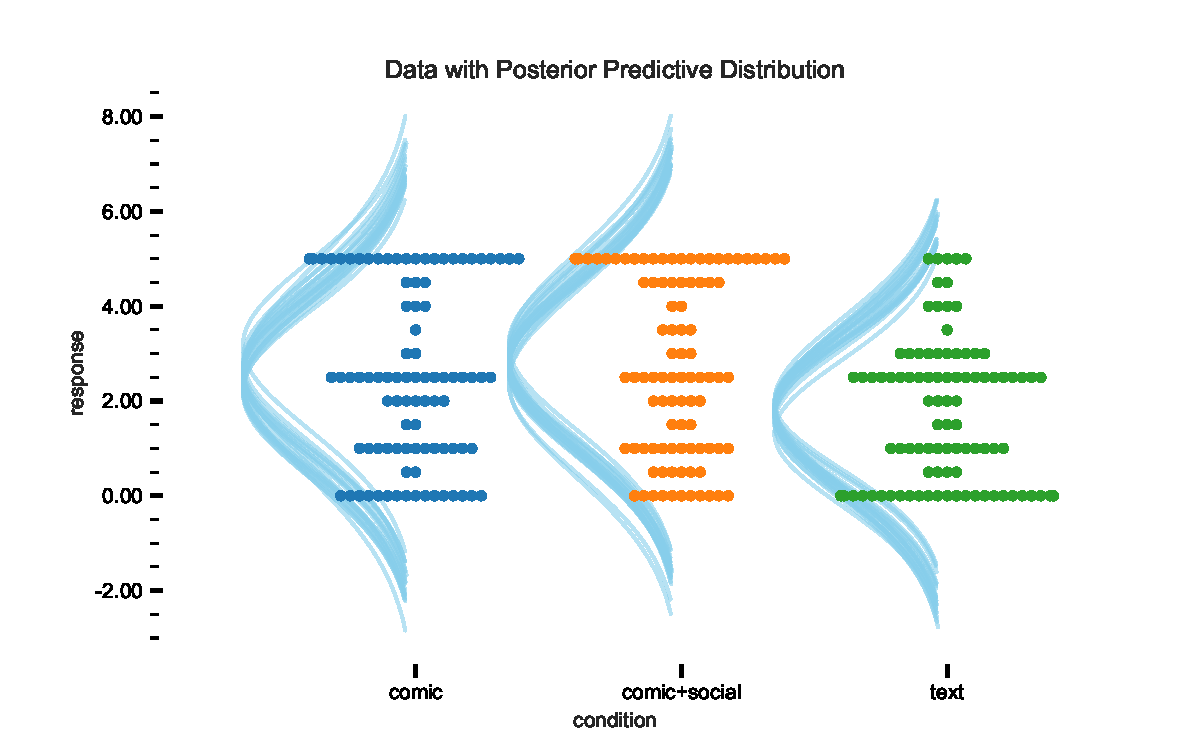
\includegraphics[width=1\textwidth]{./figures/posterior_predictions.pdf}
    \caption{Posterior prediction check: traces from the posterior distributions for each condition are super-imposed onto the observational data. The $x$-axis shows the three conditions, while the $y$-axis shows the contribution (each dot corresponds to a response by a single subject). The $t$-distribution captures the heavy tails, and we also see that the scale of the $t$-distribution in the case of the text condition is smaller than the other two cases. }
    \label{fig:posteriorprediction}
\end{figure*}

One of the advantages of a Bayesian model is that one can use the model to make predictions. Since the probabilistic model is generative, we can simply draw observations from the model. When we superimpose the posterior distribution traces onto the observational data in~\Cref{fig:posteriorprediction} we can observe three things. First, notice that the mean contribution for the `text' condition is less than the `comic' or the `comic+social norm' conditions, which seems reasonable given the increased number of \$0.0 contributions for the `text' condition in comparison to the other two cases. Second, the use of the heavy-tailed $t$-distribution captures well the tails of the distribution at \$0 and at \$5.0. Third, the scale of the distribution for the text condition is smaller than the scales for the two comic conditions, justifying our use of different scale parameters $\sigma_j$ for the three experimental conditions.


Having discussed posterior-prediction checks, next, we discuss alternatives to the model.


\subsection{Alternative Models}
\label{sub:Alternative Models}

As a first instance, consider a similar model, except that the scale parameter of the likelihood function is \textit{not nested} like our current model. Instead, we consider the equal variance case, where all the variances are equal (similar to ANOVA), and that the variance is drawn from a uniform distribution. In other words, $\sigma_j = \sigma \sim U(L, H)$, where $L>0$ and where $H$ is a large constant. The main effect of the equal variance assumption is that there is no information sharing among the groups as would be the case when each $\sigma_j$ is drawn from the same distribution, whose parameters have hyper-priors; the latter is our current model.

The main effect of constraining our simplified model is that we are slightly poorer in predicting the observed data since all the variances are guaranteed by the model to be equal, whereas we can see from~\Cref{fig:traceplot} that the mean scale (or equivalently variance) in the text condition is lower. We are skipping the traceplot and the contrast plots in this case, as they are similar, to~\Cref{fig:traceplot} and~\Cref{fig:robustcontrasts}, except that the effect size for the combined case is slightly lower due to the equal variance assumption. 

Instead, we compare the two models using WAIC (Widely Applicable Information Criterion), a principled way to compare models when they have identical likelihood functions~\parencite{Gelman2014a}. WAIC uses the predictive loss to compare two models with different parameters. First, WAIC computes the average log likelihood of each training data point (over the posterior distribution) less the variance of the log likelihood for the same data point; and then it computes the sum over all data points. That is, WAIC for a model: 

\begin{equation*}
    \mathrm{WAIC} = -2 \left (\sum_i^N \log \mathrm{Pr}(y_i) - V(y_i) \right) 
\end{equation*}

where, $N$ is the total number of training points, $y_i$ is the observation, $\mathrm{Pr}(y_i)$ is the averaged data likelihood over the posterior, and where $V(y_i)$ is the variance of the data likelihood over the posterior. When we compare the two models, one with unequal variances, and one with equal variances. We show our results in~\Cref{tab:WAIC comparison}:

\npdecimalsign{.}
\nprounddigits{2}

\begin{table}[htb]%\footnotesize
    \centering
        \caption{WAIC comparison between the model with equal variances against the case when the variances are not constrained to be equal (i.e. we use a hierarchical model). Both cases assume the Student-$t$ likelihood function, the function used in this paper. The columns show respectively, WAIC, pWAIC (the effective number of parameters; also: $\mathrm{pWAIC}=\sum_i V(y_i)$), dWAIC (the difference between the WAIC scores of the other models with the best model), weight (the relative probability that the model explains the data) SE, the standard error of the WAIC estimate, dSE is the standard error of the difference of the current model against the top model. The table shows that the hierarchical model with unequal variances better explains the observations. }\label{tab:WAIC comparison}
        \begin{tabular}{rcccccc} \toprule
            Model & WAIC & pWAIC & dWAIC & weight & SE & dSE \\ \midrule
             Unconstrained variances, hierarchical    & 1102.48    & 3.95 &     0.00 &     1.00 &     14.61 &     0.00    \\
            Constrained, equal variances & 1104.17 & 3.42 & 1.69 & 0.00 & 14.25 & 1.54        \\ \bottomrule
        \end{tabular}
    
    \end{table}

The results in~\Cref{tab:WAIC comparison} say that model with the unconstrained variances is better at explaining the data than the model with constrained variances; the relative probability that the hierarchical model with unconstrained variances better explains the observation is 1.0 (refer to the weight column in~\Cref{tab:WAIC comparison})

How useful was the choice of the Student-t drawing distribution~\Cref{eq:bayesian formulation}, instead of assuming that the outcomes are drawn from a Normal distribution? Our analysis of the posterior distribution of the degrees of freedom parameter $\nu$ shows that there is only a small probability ($P(\nu \leq 30) \approx 0.07$) that $\nu \leq 30$. Thus, we may use the Normal likelihood function, without significantly affecting the conclusions. Indeed, in our experiments, when we do model the observations with a Normal likelihood, assume equal variances, we find no significant differences in the contrasts or the effect sizes, with the Student-$t$ model with equal variances (results omitted due to space constraints).

Since the charitable donations are bounded to lie between \$0.0 and \$5.0, might we benefit from using bounded likelihood functions like the Beta distribution $Y \sim Beta(\alpha_j, \beta_j)$ to represent the charitable donations $Y_j$ under the different conditions $j$? While a $Beta(\alpha, \beta)$ distribution lies between $[0,1]$, we can scale down the contributions to lie in $[0,1]$ to use with the $Beta(\alpha, \beta)$ distribution. But notice from~\Cref{fig:contributions across conditions} that in each experimental condition, there is a central lobe, and heavy tails at each extreme, notably at \$0.0 and at \$5.0. 

%Our view of models motivated by~\textcite{McElreath2015} is that they represent an \textit{epistemological} claim, not an \textit{ontological} claim (i.e. a physical assumption about the world). Since our goal is to understand the average tendency to give to charity under the different conditions, and not to make predictions (as might be the case if we were trying to model donation with age as a predictor), the fact that the $t$-distribution is not bounded is less relevant here. 

\end{document}
